%% EPJC / Springer Nature sn-jnl conversion
%% Template: Springer Nature LaTeX template (Dec 2024), journal option [iicol]
%% Ref style: sn-mathphys-num (numbered), as recommended for math/phys EPJC
\documentclass[pdflatex,sn-mathphys-num]{sn-jnl}

\usepackage{graphicx}
\usepackage{amsmath,amssymb,bm}
\usepackage{hyperref}
%% The class default \orcid prints the Orcid logo image (Orcidlogo.eps), which
%% is not shipped with this source; typeset the identifier as a plain link.
\renewcommand{\orcid}[1]{~\href{https://orcid.org/#1}{ORCID: #1}}
\providecommand{\gtrsim}{\geq}
\providecommand{\lesssim}{\leq}

\newcommand{\MP}{M_{\rm Pl}}
\newcommand{\Ztwo}{\mathbb{Z}_2}
\newcommand{\Ztwopsi}{\Ztwo^{\psi}}
\newcommand{\PhiV}{\Phi_0}
\newcommand{\vev}[1]{\langle #1\rangle}

\theoremstyle{thmstyleone}
\newtheorem{theorem}{Theorem}

\raggedbottom

\begin{document}

\title[Induced-Gravity Cosmology]{Induced-Gravity Cosmology: Inflation, Dark Energy, and Dark Matter from a Common Scalar Origin}

%% Independent researcher: EPJC records city/country of residence.
\author*{\fnm{Yaming} \sur{Hu}}\email{64687555@qq.com}\orcid{0009-0003-1406-0485}
\affil*{\orgaddress{\city{Guiyang}, \state{Guizhou}, \country{China}}}

\abstract{We construct a scalar-tensor cosmology within pure induced gravity, in which a single real scalar field $\Phi$ with a $\Ztwo$-symmetric potential $V_J(\Phi)=\frac{\lambda_0}{4}(\Phi^2-\PhiV^2)^2+V_c$ and non-minimal coupling $\xi\Phi^2R$ replaces the Einstein--Hilbert term, generating the Planck mass via $\vev{\Phi}=\MP/\sqrt{\xi}$. Conformal transformation to the Einstein frame yields a Starobinsky-type slow-roll plateau. With locked $N\equiv\ln(a_{\rm end}/a_*)$ and exact potential slow-roll, $\xi=11.1$ gives $N=50\Rightarrow\lambda_0\simeq6.70\times10^{-8}$, $r\simeq0.00425$, $n_s\simeq0.962$; anomaly $T_{\rm reh}\simeq10^9$ GeV maps to $N\simeq50.7$. Planck $2\sigma$ selects $N\approx45$--$56$ ($r\leq0.0052$); LiteBIRD $r>0.01$ would exclude the model class. A Dirac fermion $\psi$ with $-g\Phi\bar\psi\psi$ is a cold-dark-matter \emph{candidate}: $m_\psi=g\PhiV$ shares the same VEV; stability uses a discrete $\Ztwopsi$ symmetry and a conformally vanishing $\chi\psi\bar\psi$ vertex (both structural consequences of $F=\xi\Phi^2$), conditional on an anomaly-free UV completion. Matching $\Omega_{\rm DM}$ with the exact mode-equation spectrum at the end-of-inflation transition selects $g\simeq1.0\times10^{-7}$ ($m_\psi\simeq7.5\times10^{10}$ GeV $\simeq4.6\times10^{-3}H_{\rm inf}$), cold kinematics ($\lambda_{\rm fs}\sim10^{-19}$ Mpc); absolute normalization awaits a lattice computation. The potential minimum furnishes a frozen cosmological constant with $w=-1$ (residual-condensate corrections $\leq10^{-10}$); \textbf{this dark-energy sector is calibrated, not predicted}, with $V_c$ fixed by $\Omega_\Lambda=0.683$ and the $10^{110}$ hierarchy unexplained. The identity $\Omega=\Phi/\PhiV$ decouples $\chi$ from $\psi$ at tree level; large $m_\chi\sim10^{13}$ GeV suppresses SM fifth forces. Tree-level $\chi\to h\bar h$ and $\chi\to\psi\bar\psi$ are closed; reheating is via conformal anomaly. The SM embedding is RG-stable ($\Delta\xi\leq10^{-6}$); the late-time $w_0=-1$ prediction is shared with $\Lambda$CDM and is therefore not independently discriminating, so the sharp falsification handles remain the inflationary observables.}


\keywords{induced gravity, scalar--tensor cosmology, Starobinsky plateau, gravitational particle production, superheavy dark matter, cosmological constant}

\maketitle



\section{Introduction}

Modern $\Lambda$CDM cosmology achieves remarkable observational success, yet the physical origins of its key components---inflation, dark matter, and dark energy---remain unresolved. The Einstein--Hilbert term is treated as fundamental, and the three sectors are described by independent mechanisms with no shared microphysics.

Induced gravity~\cite{Zee1979,Smolin1979} offers an elegant conceptual simplification: the Planck mass is not fundamental but emerges from the vacuum expectation value of a real scalar field $\Phi$. The Einstein--Hilbert term $M_{\rm Pl}^2R/2$ is replaced by $\xi\Phi^2R/2$; without field condensation, there is no spacetime gravity. At low energies, General Relativity is recovered as $\Phi\to\MP/\sqrt{\xi}$.

The Einstein-frame potential is shown in Fig.~\ref{fig:VE}. The domain-wall / EFT-boundary structure at $\Phi=0$ is illustrated in Fig.~\ref{fig:wall}. At large field values, the non-minimal coupling produces, after conformal transformation to the Einstein frame, a Starobinsky-type slow-roll plateau~\cite{Bezrukov2008,Starobinsky1980}. The plateau geometry follows unavoidably from the same coupling that generates $\MP$.

Once this step is taken, a single field $\Phi$ with a single $\Ztwo$-symmetric potential $V_J(\Phi)$ can simultaneously account for:
\begin{itemize}
\item \textbf{The Planck scale:} $\vev{\Phi}=\MP/\sqrt{\xi}$ gives the observed gravitational coupling.
\item \textbf{Inflation:} at $\Phi\gg\PhiV$, conformal transformation yields a Starobinsky-type plateau. Attractor forms $n_s\simeq1-2/N$ and $r\simeq8/(\beta^2N^2)$ are analytic guides; all numerical values in this paper use the locked cosmological definition $N=\ln(a_{\rm end}/a_*)$ with exact potential slow-roll (Sec.~III), which at $N=50$ gives $r\approx0.00425$ rather than the attractor $0.00487$.
\item \textbf{Dark matter:} a Dirac fermion $\psi$, with mass $m_\psi=g\PhiV$ set by the same VEV, is gravitationally produced at the end of inflation and is stable under the discrete $\Ztwopsi$ symmetry together with the conformally vanishing $\chi\psi\bar\psi$ vertex; the condensate itself decays to complete reheating. The relic abundance requires a preheating simulation (Sec.~V).
\item \textbf{Dark energy:} the residual vacuum energy $V_c$ at $\Phi=\PhiV$ gives $w=-1$ (up to residual-condensate corrections; App.~D5), \emph{calibrated empirically} to $\Omega_\Lambda$ --- not a dynamical prediction of residual inflaton motion.
\item \textbf{Fifth-force screening:} the conformal identity $\Omega=\Phi/\PhiV$ (forced by $F=\xi\Phi^2$) decouples the scalar from the dark-matter fermion $\psi$ at tree level; for Standard Model matter, the scalar's large mass $m_\chi\sim10^{13}\,$GeV (Yukawa range $\sim10^{-27}\,$cm) suppresses fifth forces, automatically satisfying solar-system bounds.
\item \textbf{$\Ztwo$ domain wall:} the surface $\Phi=0$ is a classical EFT boundary where $F(0)=F'(0)=0$ renders the Israel junction conditions inconsistent.
\end{itemize}

\textbf{Relation to existing work.} Induced gravity was originally proposed as an alternative to the Einstein--Hilbert action~\cite{Zee1979,Smolin1979} and later recognized as a natural framework for inflation~\cite{Spokoiny1984,Lucchin1985}. Recent work has explored induced-gravity inflation with various potentials~\cite{KalloshLinde,GiudiceLee2014}, while the non-minimal coupling $\xi\Phi^2R$ is shared with Higgs inflation~\cite{Bezrukov2008} (though at $\xi\sim10^4$ rather than $\xi\sim11.1$). $R^2$ (Starobinsky) inflation~\cite{Starobinsky1980} produces identical $n_s(N)$ and $r(N)$ functional forms but lacks the unified dark-energy/dark-matter embedding. The idea of unifying inflation and dark energy through a single scalar potential has been explored in quintessential inflation~\cite{PeeblesVilenkin,DimopoulosOwen}, typically with disparate scales bridged by tracker or scaling solutions. The present work differs in three respects: (a) pure induced gravity (no independent $M_{\rm Pl}^2R/2$ term) with the $\Ztwo$-symmetric double-well potential simultaneously provides the inflationary plateau, the dark-energy vacuum energy, and the dark-matter mass scale from a single VEV; (b) the conformal identity $\Omega=\Phi/\PhiV$---a structural consequence of $F=\xi\Phi^2$---closes the perturbative Yukawa reheating channel and decouples the dark-matter fermion at tree level, making gravitational particle production the sole DM source; (c) the $\chi\to h\bar h$ tree-level decay is structurally closed in induced gravity (in contrast to $R^2$ inflation), making the conformal-anomaly decay the dominant reheating channel. These features are not imposed by hand but follow unavoidably from the induced-gravity coupling. Two consequences deserve emphasis. First, since the $n_s(N)$ and $r(N)$ functions are numerically identical to those of $R^2$ inflation, the inflationary sector alone does \emph{not} discriminate this model from Starobinsky inflation at fixed $N$; what differs is the input budget, because the same VEV fixes both the Planck mass and the dark-matter mass through the exact relation $m_\psi/H_{\rm inf}=(g/\sqrt{\xi})(\MP/H_{\rm inf})$. The model's only non-degenerate observational handle is therefore the dark-matter sector, which is precisely the sector whose absolute normalization is still pending (Sec.~V). Second, the gravitational-production channel places the fermion in the wimpzilla class~\cite{ChungKolbRiotto1998,KolbChungRiotto1999,KuzminRubakov1998}, but with a quantitatively different outcome: in the standard wimpzilla treatment the relic abundance is exponentially sensitive to $m_\psi/H_{\rm inf}$ and is matched near $m_\psi\sim H_{\rm inf}$, whereas the exact mode-equation spectrum across the end-of-inflation transition is a power law (Appendix~D0), which moves the matching solution down to $m_\psi\simeq4.6\times10^{-3}H_{\rm inf}$ and makes the abundance scale with the reheating temperature rather than with $g$.

This paper constructs this unified framework. Section~II lays the theoretical foundation. Sections~III--IV cover inflation and reheating. Section~V treats the gravitationally produced fermion $\psi$ as the dark matter candidate. Section~VI derives the frozen $\Lambda$CDM dark energy. Section~VII presents the active order parameter. Section~VIII embeds the Standard Model and verifies RG stability. Section~IX analyzes the $\Ztwo$ domain wall as a classical EFT boundary. Section~X synthesizes the unified picture. Section~XI collects falsifiable predictions. Section~XII enumerates open problems.

We define the coupling function $F(\Phi)\equiv\xi\Phi^2$, central to all metric variations and junction conditions. Matter fields (fermions $\psi$) couple through Yukawa interactions $\mathcal{L}_Y=-g\Phi\bar\psi\psi$, with $m_\psi=g|\Phi|$. In this paper, ``common origin'' refers to the fact that all relevant mass scales---the Planck mass $\MP$, the dark-matter fermion mass $m_\psi=g\PhiV$, and the overall scale of $V_J(\Phi)$---are set by a single vacuum expectation value $\vev{\Phi}=\PhiV$; the dark matter is a fermionic partner whose stability is guaranteed by the same UV gauge structure (the discrete $\Ztwopsi$ symmetry). We do not claim a microphysical derivation of the dark-energy scale $V_c$, which is calibrated empirically.

\section{Theoretical foundation}

\subsection{Action and field equations}

We adopt the $(-,+,+,+)$ metric signature and the Landau--Lifshitz curvature conventions ($R^\rho_{\ \sigma\mu\nu}=\partial_\mu\Gamma^\rho_{\nu\sigma}-\cdots$, $R_{\mu\nu}=R^\rho_{\ \mu\rho\nu}$, $R=g^{\mu\nu}R_{\mu\nu}$).

The Jordan-frame action is
\begin{equation}
S=\int d^4x\sqrt{-g}\left[\frac12\xi\Phi^2R-\frac12 g^{\mu\nu}\partial_\mu\Phi\partial_\nu\Phi-V(\Phi)\right]+S_{\rm matter},
\label{eq:action}
\end{equation}
with the symmetry-breaking potential
\begin{equation}
V(\Phi)=\frac{\lambda_0}{4}\left(\Phi^2-\PhiV^2\right)^2+V_c,
\qquad
\PhiV=\frac{\MP}{\sqrt{\xi}},
\label{eq:potential}
\end{equation}
where $V_c$ is a vacuum-energy constant, $\MP\approx2.435\times10^{18}\,$GeV, and $\lambda_0$ is the self-coupling. The $\Ztwo$ symmetry $\Phi\to-\Phi$ produces degenerate vacua $\pm\PhiV$ separated by a potential barrier at $\Phi=0$.

Variation with respect to $g_{\mu\nu}$ yields the modified Einstein equation
\begin{equation}
F G_{\mu\nu}=T^{\rm matter}_{\mu\nu}+T^{(\Phi)}_{\mu\nu}+\nabla_\mu\nabla_\nu F-g_{\mu\nu}\Box F,
\label{eq:einstein}
\end{equation}
with canonical scalar energy-momentum tensor $T^{(\Phi)}_{\mu\nu}\equiv\partial_\mu\Phi\partial_\nu\Phi-\frac12 g_{\mu\nu}(\partial\Phi)^2-g_{\mu\nu}V(\Phi)$. The scalar equation of motion is
\begin{equation}
\Box\Phi-V'(\Phi)+\xi\Phi R=0.
\label{eq:scalareom}
\end{equation}

We distinguish three field variables: the Jordan-frame field $\Phi$; the logarithmic parameter $\varphi\equiv\ln(\Phi/\PhiV)$ with conformal factor $\Omega^2=e^{2\varphi}$; and the Einstein-frame canonical field $\chi$ ($d\chi/d\varphi=\MP\sqrt{6+1/\xi}$).

\subsection{$\Ztwo$ symmetry and double vacua}

The action is invariant under $\Phi\to-\Phi$; extrema satisfy $\Phi\in\{0,\pm\PhiV\}$. The domain-wall tension is
\begin{equation}
\sigma_{\rm wall}=\int_{-\PhiV}^{+\PhiV}d\Phi\sqrt{2[V(\Phi)-V(\PhiV)]}
=\frac43\sqrt{\frac{\lambda_0}{2}}\,\PhiV^3>0.
\label{eq:sigma}
\end{equation}

Cosmological domain-wall networks are avoided through initial-condition locking during inflation and inflationary dilution: since $m_\Phi=\sqrt{2\lambda_0}\PhiV\simeq2.7\times10^{14}\,$GeV $\gg H_{\rm inf}\simeq1.64\times10^{13}\,$GeV, the field relaxes to one vacuum branch ($+\PhiV$ or $-\PhiV$) within a few $m_\Phi^{-1}$, well before the CMB scales exit the horizon; inflation then stretches this choice beyond the present horizon, so the standard post-inflationary Kibble wall-formation argument does not apply. The relevant suppression is in \emph{number density}, not energy density: the number of walls per comoving volume is diluted by $n_{\rm wall}\propto a^{-3}\sim e^{-3N}$, giving a probability $\sim e^{-3N}\sim10^{-65}$ that a single wall intersects our observable patch. (For completeness: the wall tension $\sigma_{\rm wall}\sim(4/3)\sqrt{\lambda_0/2}\,\PhiV^3\sim10^{50}\,$GeV$^3$ vastly exceeds the CMB bound $\sigma\leq(1\,{\rm MeV})^3$, so any wall in our patch would be catastrophic---but the number-density suppression by inflation makes this exponentially unlikely.) Bias-potential elimination remains an open problem.

\subsection{Unified mass scales from the scalar VEV}

The key unification mechanism is that all mass scales originate from the VEV of $\Phi$:

\paragraph{a. Planck mass.} The effective gravitational constant is
\begin{equation}
G_{\rm eff}=\frac{1}{8\pi\xi\Phi^2}
\quad\Longrightarrow\quad
G_N=\frac{1}{8\pi\xi\PhiV^2}.
\label{eq:Geff}
\end{equation}
At $\Phi=\PhiV$, $G_{\rm eff}=G_N$ matches Newton's constant. The active order parameter is $\mathcal{A}\equiv(\Phi/\PhiV)^2$, with $G_{\rm eff}=G_N/\mathcal{A}$.

\paragraph{On the relation $M_{\rm Pl}^2=\xi\PhiV^2$.} In induced gravity this is a definition, not a tuning: the Planck mass is not an independent input but is generated by the VEV, $M_{\rm Pl}^2\equiv\xi\vev{\Phi}^2$. The potential $V(\Phi)=\frac{\lambda_0}{4}(\Phi^2-\PhiV^2)^2+V_c$ has its extrema at $\Phi=\pm\PhiV$ exactly (the constant $V_c$ does not shift the minimum), so the VEV coincides with $\PhiV$ as a consequence of the potential's construction. A quantum shift of the VEV would rescale $\MP$ proportionally, leaving the dimensionless identity $\Omega=\Phi/\PhiV$ (Eq.~\eqref{eq:Omega})---which depends only on the coupling form $F=\xi\Phi^2$, not on the numerical value of $\PhiV$---intact. The conformal decoupling derived in Sec.~II E is therefore a structural property of the induced-gravity coupling, not a fine-tuned coincidence.

\paragraph{b. Fermion masses.} Fermions $\psi$ couple through the Yukawa interaction $\mathcal{L}_Y=-g\Phi\bar\psi\psi$, giving $m_\psi=g|\Phi|$. At the minimum, $m_\psi^{(0)}=g\PhiV$. A full Standard Model embedding (including Higgs-mediated masses and RG stability) is constructed in Sec.~VIII.

\paragraph{c. Weak scale (optional Higgs portal).} If a Higgs portal $\lambda_{\Phi H}\Phi^2|H|^2$ is included, the Higgs VEV becomes
\begin{equation}
v_H^2=\frac{\mu_H^2-\lambda_{\Phi H}\PhiV^2}{2\lambda_H},
\label{eq:vH}
\end{equation}
linking the electroweak scale to $\PhiV$ and hence to $\MP$. This preserves the $\Ztwo$ symmetry ($\Phi^2$ is even) and is technically natural~\cite{tHooft1980}.

\subsection{Conformal transformation to Einstein frame}

Under $\tilde g_{\mu\nu}=\Omega^2 g_{\mu\nu}=e^{2\varphi}g_{\mu\nu}$ with $\Omega^2\equiv\xi\Phi^2/\MP^2$, the exact Einstein-frame potential is
\begin{equation}
V_E(\varphi)=\frac{\lambda_0\MP^4}{4\xi^2}\left(1-e^{-2\varphi}\right)^2+V_c e^{-4\varphi}.
\label{eq:VE}
\end{equation}

Two limits: $\varphi\gg1$ gives $V_E\to\lambda_0\MP^4/(4\xi^2)\equiv V_0$ (inflationary plateau); $\varphi\to0$ gives $V_E\to V_c$ (frozen cosmological constant).

With the canonical field $\chi$, the potential assumes the Starobinsky form~\cite{Starobinsky1980}
\begin{equation}
\frac{d\chi}{d\varphi}=\MP\sqrt{6+\frac1\xi},
\qquad
V_E(\chi)=\frac{\lambda_0\MP^4}{4\xi^2}\left(1-e^{-\beta\chi/\MP}\right)^2,
\quad
\beta\equiv\frac{2}{\sqrt{6+1/\xi}},
\label{eq:VEchi}
\end{equation}
where $\beta\simeq0.810$ for $\xi\sim11.1$. The $V_c$ term is negligible on the plateau but determines the late-time dark-energy density.

\begin{figure}[t]
\centering
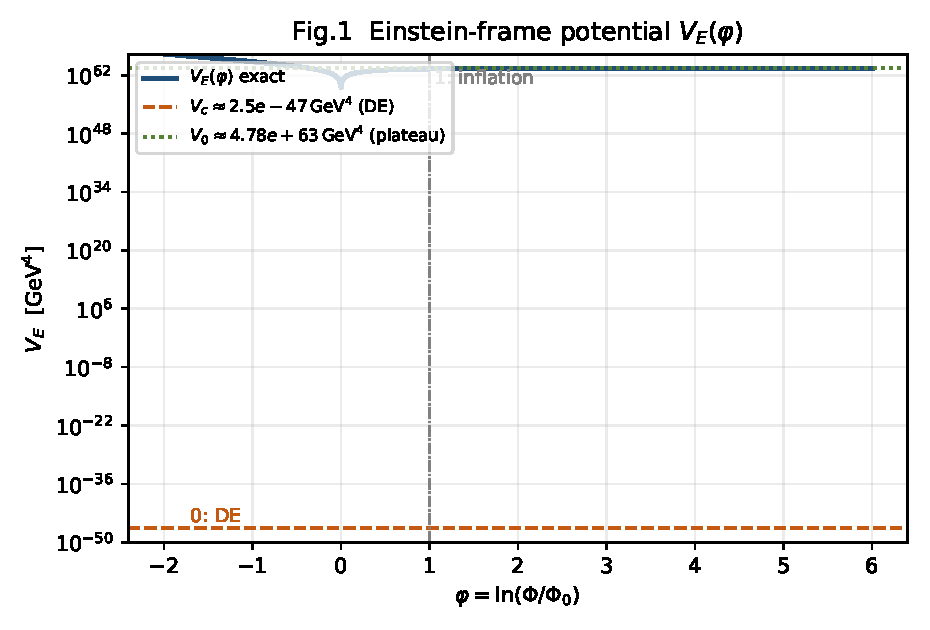
\includegraphics[width=0.95\columnwidth]{figures/fig1_VE_potential.pdf}
\caption{Exact Einstein-frame potential $V_E(\varphi)$ for locked $N=50$, $\xi=11.1$ ($\lambda_0\simeq6.70\times10^{-8}$ from exact slow-roll $A_s$). The flat plateau at $\varphi\gg1$ ($\sim V_0$) drives slow-roll inflation; the minimum at $\varphi\simeq0$ is set by the calibrated $V_c$. The hierarchy $V_0/V_c\sim10^{110}$ is spanned by the conformal factor $e^{-4\varphi}$ but not dynamically explained. Regenerated by \texttt{scripts/fig1\_einstein\_potential.py}.}
\label{fig:VE}
\end{figure}

\subsection{Conformal decoupling and automatic fifth-force screening}

A single exact identity of this model decouples the scalar field from the dark-matter fermion $\psi$, while the scalar's large mass screens the fifth force for Standard Model matter. Because $F(\Phi)=\xi\Phi^2$, the conformal factor is exactly proportional to the field:
\begin{equation}
\Omega=\frac{\sqrt{\xi}\Phi}{\MP}=\frac{\Phi}{\PhiV}
\quad\Longrightarrow\quad
\Phi=\PhiV\,\Omega,
\qquad\text{(exact, all $\Phi$)}.
\label{eq:Omega}
\end{equation}
This proportionality is specific to the induced-gravity coupling; a generic $F(\Phi)$ would not enjoy it.

We distinguish two classes of fermions. For fermions whose mass arises entirely from the direct Yukawa coupling $-g\Phi\bar\psi\psi$, the conformal identity produces exact decoupling. Under $\tilde g_{\mu\nu}=\Omega^2 g_{\mu\nu}$ and $\tilde\psi=\Omega^{-3/2}\psi$ (equivalently $\psi=\Omega^{3/2}\tilde\psi$), the Yukawa term transforms as
\begin{equation}
-g\Phi\bar\psi\psi\sqrt{-g}\longrightarrow -g\PhiV\bar{\tilde\psi}\tilde\psi\sqrt{-\tilde g}:
\label{eq:Ytrans}
\end{equation}
the $\Omega$ factors cancel exactly ($\Omega\cdot\Omega^3\cdot\Omega^{-4}=1$), giving an \emph{exact}, $\chi$-independent Einstein-frame fermion mass $m_E=g\PhiV$. The tree-level $\chi\bar{\tilde\psi}\tilde\psi$ coupling therefore vanishes identically, so the PPN parameter $\gamma=1$ holds exactly within the $\psi$ sector. At loop level, graviton exchange can induce an effective $\chi\psi\bar\psi$ vertex of parametric size $\leq m_\psi m_\chi/\MP^2\sim10^{-11}g$---utterly negligible for reheating, dark matter production, and fifth-force tests, so the tree-level vanishing is the operative feature. This $\psi$-sector decoupling is observationally inert for solar-system tests, which probe Standard Model matter (no $\psi$ sources are present in the solar system); it is instead decisive for the reheating and dark-matter analysis (Secs.~IV--V).

Standard-model fermions obtain their mass through the Higgs mechanism, so the conformal identity does \emph{not} cancel their $\chi$ coupling; a residual coupling $\sim m_f/\MP$ remains (treated separately in Sec.~VIII). The solar-system fifth-force bound is satisfied by the dominant screening mechanism, namely the scalar's large canonical mass near the minimum,
\begin{equation}
m_\chi^2=\frac{V_E''(0)}{\MP^2(6+1/\xi)}\approx\frac{2\lambda_0\MP^2}{\xi^2(6+1/\xi)}\approx(3.25\times10^{13}\,{\rm GeV})^2,
\label{eq:mchi}
\end{equation}
(at locked $N=50$, $\xi=11.1$; $3.19\times10^{13}\,$GeV at $N=51$),
which gives a Yukawa range $m_\chi^{-1}\sim10^{-27}\,$cm, exponentially suppressing any residual interaction at macroscopic distances and satisfying the Cassini bound $|\gamma-1|<2.3\times10^{-5}$~\cite{Bertotti2003}. This short-range suppression is the same mechanism operative in any heavy-scalar-tensor theory; it is distinct from a chameleon field-environment mechanism, which is not invoked here.

\paragraph{Key differences from standard Higgs inflation.} While the plateau geometry is shared: (a) $\xi\sim11.1$ is two orders below $\xi\sim10^4$, yielding a different unitarity regime; (b) $\MP$ is dynamically generated via induced gravity; (c) the same $V_J(\Phi)$ supplies both the inflationary plateau and the late-time vacuum constant $V_c$; (d) $\Phi$ is a gauge singlet, so the large top-Yukawa term that drives the Higgs $\beta_\xi$ is absent.

\subsection{EFT cutoff scale}

The status of the cutoff is frame-dependent and, for non-minimal scalar-tensor inflation, \emph{contested}. From the Einstein-frame EFT perspective~\cite{Bezrukov2008}, the action is standard GR plus a canonical scalar; higher operators are suppressed by $\MP$ and $H_{\rm inf}\ll\MP$ ensures self-consistency. From the Jordan-frame perspective~\cite{Burgess2009,Burgess2010}, the cutoff is $\Lambda_J\sim\MP/\xi\sim2.2\times10^{17}\,$GeV, and the CMB pivot value $\Phi_{\rm CMB}$ exceeds it by $\sim30$. Whether the low Jordan-frame cutoff persists as a physical limitation of the Einstein-frame EFT is an open question without community consensus~\cite{Flanagan2004}. We adopt the Einstein-frame EFT perspective for computing slow-roll observables (where they are robust) and flag the Jordan-frame cutoff tension as an open issue (Discussion \#8).

\section{Inflation: Starobinsky-type slow-roll plateau}

\paragraph{Conditional statement.} The derivation describes the geometric fact that a slow-roll plateau exists whenever $\chi\gg\MP$. The naturalness of this initial condition is not endogenously explained (Discussion \#1).

\subsection{Energy scale and CMB normalization}

\paragraph{Definition of $N$ and CMB normalization.} Throughout this paper the $e$-fold number is the cosmological quantity
\begin{equation}
N\equiv\ln\!\left(\frac{a_{\rm end}}{a_*}\right),
\qquad
k_*=a_*H_*,
\label{eq:Ndef}
\end{equation}
with pivot $k_*=0.05\,{\rm Mpc}^{-1}$. Post-inflationary matching assumes matter-like ($w=0$) condensate domination until $T_{\rm reh}$,
\begin{equation}
a_{\rm end}=a_{\rm reh}\left(\frac{\rho_{\rm reh}}{\rho_{\rm end}}\right)^{1/3},
\qquad
a_{\rm reh}=a_{\rm eq}\left(\frac{g_{*s,\rm eq}}{g_{*s,\rm reh}}\right)^{1/3}\frac{T_{\rm eq}}{T_{\rm reh}},
\qquad
a_{\rm eq}=\frac{\Omega_r}{\Omega_m},
\label{eq:matchN}
\end{equation}
with $\Omega_m\simeq0.315$, $\Omega_r\simeq9\times10^{-5}$, $\rho_{\rm reh}=(\pi^2/30)g_*T_{\rm reh}^4$, $\rho_{\rm end}=K_{\rm end}+V_{\rm end}$, $g_{*s,\rm reh}=106.75$, $g_{*s,\rm eq}=3.91$, $g_{*,\rm eq}=3.36$ and $T_{\rm eq}=(30\rho_{\rm eq}/\pi^2g_{*,\rm eq})^{1/4}$. The radiation era is matched by comoving-entropy conservation rather than by the constant-$g_*$ scaling $a\propto\rho^{-1/4}$; because $g_{*s}$ falls from $106.75$ to $3.91$ between $T_{\rm reh}$ and $T_{\rm eq}$, the two routes differ by a factor $2.04$ in $T_{\rm reh}^*$, i.e.\ $0.23$ $e$-folds in $N$. At a given $N$, the plateau variable $x_*$ is fixed by the exact potential-slow-roll integral
\begin{equation}
N=\frac{e^{x_*}-x_*-\bigl(e^{x_{\rm end}}-x_{\rm end}\bigr)}{2\beta^2},
\qquad
e^{-x_{\rm end}}=\frac{1}{1+\sqrt2\,\beta},
\qquad
\beta\equiv\frac{2}{\sqrt{6+1/\xi}},
\label{eq:Nint}
\end{equation}
and observables are evaluated at that $x_*$:
\begin{equation}
r=16\varepsilon_*,
\qquad
n_s=1-6\varepsilon_*+2\eta_*,
\qquad
A_s=\frac{V_0(1-e^{-x_*})^2}{24\pi^2\MP^4\varepsilon_*},
\label{eq:obsPS}
\end{equation}
with
\begin{equation}
\varepsilon=\frac{2\beta^2e^{-2x}}{(1-e^{-x})^2},
\qquad
\eta=\frac{2\beta^2e^{-x}(2e^{-x}-1)}{(1-e^{-x})^2},
\qquad
V_0=\frac{\lambda_0\MP^4}{4\xi^2}.
\end{equation}
Solving $A_s=2.100\times10^{-9}$ at fixed $(N,\xi)$ determines $\lambda_0$ uniquely (linear in $\lambda_0$ at fixed $x_*$). Attractor-style closed forms $r\simeq8/(\beta^2N^2)$, $n_s\simeq1-2/N$ remain useful approximations but \emph{must not} be mixed with this $N$ definition: at $N=50$ the exact potential slow-roll gives $r\approx0.00425$, whereas the closed form yields $r\approx0.00487$.

\paragraph{Fiducial point.} For $\xi=11.1$ and $N=50$ under Eq.~\eqref{eq:Ndef}:
\begin{equation}
\lambda_0\simeq6.70\times10^{-8},\quad
r\simeq0.00425,\quad
n_s\simeq0.9616,
\end{equation}
\begin{equation}
H_{\rm inf}=\sqrt{\frac{V_0}{3\MP^2}}\simeq1.64\times10^{13}\,{\rm GeV},\quad
U^{1/4}\simeq8.3\times10^{15}\,{\rm GeV},\quad
m_\chi\simeq3.25\times10^{13}\,{\rm GeV},
\label{eq:scales_locked}
\end{equation}
where $m_\chi^2=8V_0/(\MP^2\beta_o^2)=2\lambda_0\MP^2/[\xi^2(6+1/\xi)]$ with $\beta_o=\sqrt{6+1/\xi}$. The conformal-anomaly reheating estimate $T_{\rm reh}\sim10^9\,$GeV maps through Eqs.~\eqref{eq:matchN}--\eqref{eq:Nint} to $N\simeq50.7$ (not 50); the corresponding self-consistent temperature for $N=50$ is $T_{\rm reh}\simeq1.1\times10^{8}\,$GeV. Matching assumptions ($k_*$, $w$ during reheating, $\Omega$'s) shift these temperatures by $\mathcal{O}(1)$--$\mathcal{O}(10)$.

\paragraph{Sensitivity table.} Table~\ref{tab:sens} lists exact slow-roll predictions at $\xi=11.1$ under the locked $N$ definition. Planck $2\sigma$ ($n_s\in[0.9565,0.9733]$) selects $N\approx45$--$56$ with $r\in[0.0034,0.0052]$; the tighter $1\sigma$ lower edge $n_s\geq0.9607$ selects $N\geq49$. The upper edge is not set by $n_s$ but by reheating: the tabulated $T_{\rm reh}^*(N)$ grows as $e^{3.05N}$, so $T_{\rm reh}^*(56)\simeq7.8\times10^{15}\,$GeV already exceeds the instantaneous-reheating ceiling $T_{\rm reh}^{\rm inst}=(30\rho_{\rm end}/\pi^2g_*)^{1/4}\simeq2.6\times10^{15}\,$GeV obtained at $N=56$; hence $N_{\rm max}\simeq55.6$ and $N=57,58$ are physically excluded (Appendix~D).

\paragraph{Two-sided physical window.} The admissible band is bounded on \emph{both} sides by physics, not by the $n_s$ likelihood alone. On the high side, $T^*_{\rm reh}(N)\propto e^{3N}$ while the instantaneous-reheating ceiling falls only as $N^{-1/2}$, giving $N_{\rm max}\simeq55.6$ as shown above. On the low side, the model cannot be pushed to small $N$: the tensor-to-scalar ratio falls to $r=0.01$ at $N_*\simeq32$ in the locked-$N$ convention (the attractor closed form $r\simeq8/(\beta^2N^2)$ gives $N_*\simeq35$), so $r>0.01$ requires $N\lesssim32$, for which the matching condition \eqref{eq:matchN} returns $T_{\rm reh}\simeq5.9\times10^{-17}\,$GeV---fourteen orders of magnitude below the BBN floor of $10\,$MeV---so such a point is physically impossible for any reheating mechanism. The viable interval is therefore $N\in[45,55.6]$, and Planck $2\sigma$ on $n_s$ happens to select almost exactly that range. This is what makes the model falsifiable in a definite way: a LiteBIRD-class detection $r>0.01$ would demand $N\lesssim32$ and hence a reheating temperature incompatible with BBN, so it would exclude the model class outright rather than merely disfavour it.

\paragraph{Reheating equation of state and the $N$--$T_{\rm reh}$ mapping.} The mapping above assumes the condensate behaves as pressureless dust ($w=0$) throughout the post-inflationary phase. This is an approximation: the potential is not exactly harmonic at the largest amplitudes (Appendix~D), and the exact integration of Sec.~D\,0 gives $\langle w\rangle\simeq-0.02$ averaged over the first few $e$-folds, approaching zero thereafter. A constant-$w$ reheating epoch with $\bar w_{\rm eff}$ shifts the $e$-fold count by $\Delta N=\frac{1-3\bar w_{\rm eff}}{12(1+\bar w_{\rm eff})}\ln(T_{\rm reh}/T_{\rm end})$; for $\bar w_{\rm eff}\in[0,1/3]$ this gives $|\Delta N|\lesssim1$, so the mapping is stable at the stated $\mathcal{O}(1)$ level and the quoted band is unaffected.

\paragraph{Quantum diffusion.} During slow-roll, quantum fluctuations cause the field to undergo a random walk with variance $\langle\delta\chi^2\rangle\simeq H_{\rm inf}^3 t/(4\pi^2)$ per Hubble time. Over one $e$-fold $\Delta t=H_{\rm inf}^{-1}$, the accumulated quantum jitter is $\Delta\chi_{\rm quant}\sim H_{\rm inf}/(2\pi)$, while the classical drift is $\Delta\chi_{\rm class}\sim\dot\chi/H_{\rm inf}\sim\MP\sqrt{2\epsilon}$. The ratio $\Delta\chi_{\rm quant}/\Delta\chi_{\rm class}\sim H_{\rm inf}/(2\pi\MP\sqrt{2\epsilon})\sim6\times10^{-6}/\sqrt{\epsilon}$ is utterly negligible except at the very end of inflation ($\epsilon\to1$), where it reaches $\sim6\times10^{-6}$---still five orders below unity. Stochastic effects therefore do not invalidate the classical slow-roll trajectory for this model.

\paragraph{Attractor forms and non-Gaussianity.} Large-field attractor expressions $n_s\simeq1-2/N$, $r\simeq8/(\beta^2N^2)$, $n_t=-r/8$ are useful analytic guides; numerical values quoted in Table~\ref{tab:sens} use the exact integral \eqref{eq:Nint} and potential slow roll \eqref{eq:obsPS} at the locked $N$. Being of the Starobinsky type, the model also predicts negligible primordial non-Gaussianity: $f_{\rm NL}^{\rm local}=-\frac{5}{12}(1-n_s)\sim-0.02$, with equilateral and orthogonal shapes suppressed by the slow-roll parameters to $\mathcal{O}(10^{-2})$, all well within Planck 2018 constraints~\cite{Planck2018} ($f_{\rm NL}^{\rm local}=-0.9\pm5.1$).

\begin{table}[t]
\centering
\caption{Exact potential slow-roll at $\xi=11.1$ under the locked definition $N=\ln(a_{\rm end}/a_*)$ (Eqs.~\eqref{eq:Ndef}--\eqref{eq:obsPS}). $\lambda_0$ is fixed by $A_s=2.100\times10^{-9}$. $T_{\rm reh}^*$ is the temperature for which cosmological matching \eqref{eq:matchN} returns $N_{\rm derived}=N$. Planck $2\sigma$ allows $N\approx45$--$56$ ($r\leq0.0052$).}
\label{tab:sens}
\begin{tabular}{c|c|c|c|c|c}
$N$ & $\lambda_0$ & $n_s$ & $r$ & $H_{\rm inf}$ [GeV] & $T_{\rm reh}^*$ [GeV] \\
\hline
48 & $7.24\times10^{-8}$ & 0.9600 & 0.00459 & $1.70\times10^{13}$ & $2.6\times10^{5}$ \\
49 & $6.96\times10^{-8}$ & 0.9608 & 0.00441 & $1.67\times10^{13}$ & $5.2\times10^{6}$ \\
50 & $6.70\times10^{-8}$ & 0.9616 & 0.00425 & $1.64\times10^{13}$ & $1.1\times10^{8}$ \\
51 & $6.45\times10^{-8}$ & 0.9623 & 0.00409 & $1.61\times10^{13}$ & $2.2\times10^{9}$ \\
52 & $6.21\times10^{-8}$ & 0.9630 & 0.00394 & $1.58\times10^{13}$ & $4.5\times10^{10}$ \\
55 & $5.58\times10^{-8}$ & 0.9650 & 0.00355 & $1.50\times10^{13}$ & $3.8\times10^{14}$ \\
\end{tabular}
\end{table}

\subsection{Slow-roll parameters and observables}

In the $\chi\gg\MP$ limit, the potential slow-roll parameters are
\begin{align}
\epsilon_V&\equiv\frac{\MP^2}{2}\left(\frac{V_E'}{V_E}\right)^2
\simeq2\beta^2 e^{-2\beta\chi/\MP}\ll1,\\
\eta_V&\equiv\MP^2\frac{V_E''}{V_E}
\simeq-2\beta^2 e^{-\beta\chi/\MP},\\
N&\simeq\frac{e^{\beta\chi_N/\MP}}{2\beta^2}.
\label{eq:slowroll}
\end{align}
We use the potential slow-roll (PSR) formulation throughout; the Hubble slow-roll (HSR) parameters $\epsilon_H\equiv-\dot H/H^2$ and $\eta_H\equiv\ddot\chi/(H\dot\chi)$ coincide with $\epsilon_V$ and $\eta_V$ to leading order in slow-roll, with relative differences $\Delta\epsilon/\epsilon\sim\mathcal{O}(\epsilon,\eta)\leq10^{-2}$ in the deep slow-roll regime and rising to $\sim\mathcal{O}(1)$ only at the very end of inflation ($\epsilon\to1$). The $e$-fold number $N$---the quantity that enters the CMB observables---is insensitive to the PSR/HSR distinction at the $\leq0.1$ level, well within the $\mathcal{O}(1)$ systematic uncertainty already quoted for the post-inflationary phase.

\paragraph{Cutoff disclaimer.} The slow-roll expressions are leading-order results in the Einstein-frame EFT ($\Lambda_E\sim\MP$). Higher-derivative corrections enter at order $(H_{\rm inf}/\MP)^2\sim3\times10^{-11}$; the functional forms $n_s(N)$ and $r(N)$ are insensitive to the cutoff.

\paragraph{Perturbation stability.} In the Einstein frame the scalar field $\chi$ is canonically normalized with a standard kinetic term $\frac12(\partial\chi)^2$, so the scalar sound speed is $c_s^2=1$ identically---no gradient instability can arise. The tensor sector is standard GR with $c_T=1$ (see also Discussion \#16). The comoving curvature perturbation $\zeta$ is conserved on superhorizon scales for adiabatic single-field models~\cite{LiddleLyth2000}; no entropy/isocurvature modes are sourced because the single field $\Phi$ drives both the background and the perturbations. The standard single-field slow-roll formulas for $n_s$, $r$, and the scalar power spectrum therefore apply without modification.

The scalar spectral index with NLO correction is
\begin{equation}
n_s\simeq1-\frac{2}{N}-\frac{3}{2N^2}+\mathcal{O}(N^{-3}).
\label{eq:ns}
\end{equation}
(The NLO coefficient $-\frac{3}{2}$ applies in the Starobinsky limit $\beta=\sqrt{2/3}$; for general $\beta$ it acquires a $\beta$-dependence. \textbf{All tabulated $n_s$ and $r$ in this paper use the exact potential slow-roll evaluation \eqref{eq:obsPS} at the locked $N$, not this NLO closed form.} A quantitative slow-roll scan shows the NLO closed form differs from exact PS by $\leq3\times10^{-4}$ in $n_s$ at $\xi=11.1$ ($\beta=0.810$) and throughout $\xi\geq 5$---well below Planck $\sigma(n_s)=0.0042$---but the shift grows toward $\xi\to1$; precision comparisons at small $\xi$ must use the exact integral \eqref{eq:Nint}.)

For the locked definition, exact potential slow roll at $\xi=11.1$ gives $n_s\simeq0.9616$ at $N=50$ ($-0.79\sigma$ from Planck) and $n_s\simeq0.9650$ at $N=55$ ($+0.02\sigma$); see Table~\ref{tab:sens}. Planck 2018~\cite{Planck2018}: $0.9649\pm0.0042$ ($1\sigma$). The prediction approaches the Planck central value as $N$ increases; the $2\sigma$ band corresponds to $N\approx45$--$56$ in this convention.

The tensor-to-scalar ratio under the same convention is $r\simeq0.00425$ at $N=50$ and $r\simeq0.00355$ at $N=55$; across Planck $2\sigma$ $N\approx45$--$56$, $r\in[0.0034,0.0052]$. Planck+BICEP/Keck~\cite{Planck2018,BICEP2021}: $r<0.036$ (95\% CL).

A measurement $r>0.01$ at 95\% CL by LiteBIRD~\cite{LiteBIRD2023} would rule out the entire physically allowed model class in this convention: exact slow-roll inversion puts $r=0.01$ at $N\approx32$ (for $\xi=11.1$), outside the Planck-compatible band, and reheating temperatures required for such small $N$ fall far below BBN. Throughout the $2\sigma$ window, $r\leq0.0052$ at $\xi=11.1$ (only weakly $\xi$-dependent once $x_*(N)$ is fixed by the exact integral).

Figure~\ref{fig:nsr} shows the model predictions superimposed on Planck+BICEP/Keck-style constraints.

\begin{figure}[t]
\centering
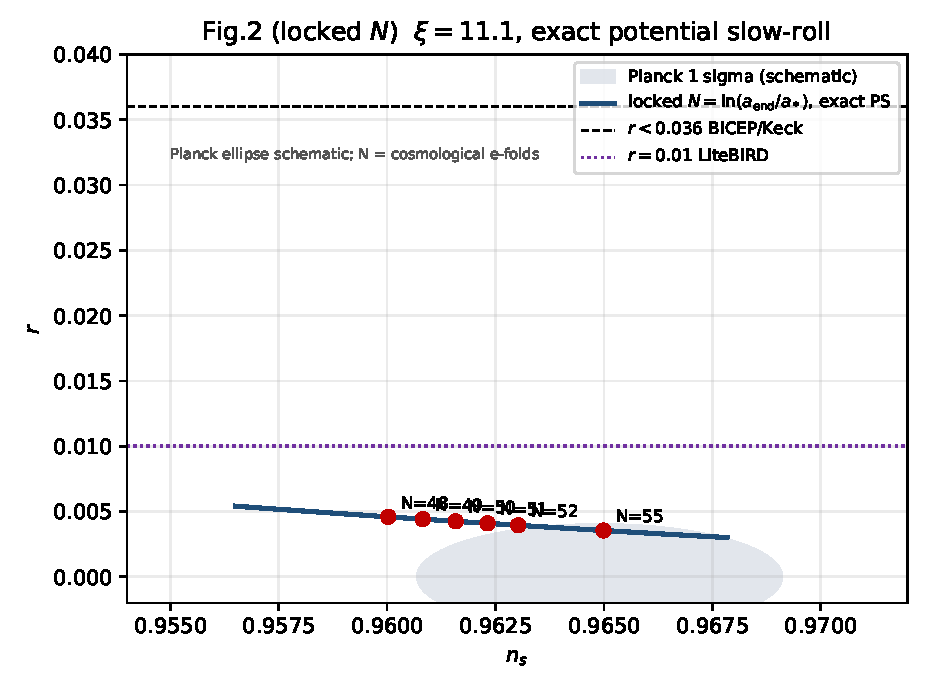
\includegraphics[width=0.95\columnwidth]{figures/fig2_ns_r.pdf}
\caption{$n_s$--$r$ under the locked definition $N=\ln(a_{\rm end}/a_*)$ at $\xi=11.1$ (exact potential slow-roll, $\lambda_0$ from $A_s$; Table~\ref{tab:sens}). Markers: locked-$N$ points. Planck ellipse schematic; BICEP/Keck $r<0.036$; LiteBIRD line $r=0.01$. Regenerated by \texttt{scripts/fig2\_ns\_r.py} (locked-N convention; same as \texttt{lock\_n\_convention.py}).}
\label{fig:nsr}
\end{figure}

\section{End of slow-roll and reheating}

\subsection{End of slow-roll and coherent oscillations}

Slow-roll ends at $\epsilon=1$. The exact $\epsilon$ derived from $V_E=V_0(1-e^{-\beta\chi/\MP})^2$ is $\epsilon_{\rm exact}=2\beta^2 e^{-2x}/(1-e^{-x})^2$ with $x\equiv\beta\chi/\MP$; the large-field limit $(1-e^{-x})\approx1$ reduces it to Eq.~\eqref{eq:slowroll}. Solving $\epsilon_{\rm exact}=1$ with $u\equiv e^{-x}$ gives $u=1/(1+\sqrt{2}\beta)\approx0.466$, so
\begin{equation}
\begin{aligned}
e^{-\beta\chi_{\rm end}/\MP}&=\frac{1}{1+\sqrt{2}\beta}\approx0.466,\\
V_{\rm end}&=V_0\left(1-e^{-\beta\chi_{\rm end}/\MP}\right)^2\approx0.285\,V_0\approx1.36\times10^{63}\,{\rm GeV}^4\\
&\qquad(V_0\simeq4.78\times10^{63}\,{\rm GeV}^4\ \text{at locked }N=50).
\end{aligned}
\label{eq:Vend}
\end{equation}
Thereafter the field oscillates around $\PhiV$ with mass $m_\Phi=\sqrt{2\lambda_0}\PhiV\approx2.7\times10^{14}\,$GeV. Near the minimum, $V_J(\Phi)\approx\lambda_0\PhiV^2(\Phi-\PhiV)^2+\mathcal{O}((\Phi-\PhiV)^3)$, i.e.\ the potential is quadratic to leading order; the quartic $(\Phi^2-\PhiV^2)^2$ form produces a radiation-like equation of state ($w\simeq1/3$) only for oscillations around $\Phi=0$, which is never reached since the field is confined to one vacuum branch ($+\PhiV$ or $-\PhiV$) by the initial-condition locking of Sec.~II. Consequently the amplitude redshifts as $A(t)\propto a^{-3/2}$ and the condensate evolves as pressureless dust ($w=0$). This last statement is an approximation: the post-inflationary excursion reaches $|x|\equiv|\beta\chi/\MP|\simeq0.88$ (Sec.~III and App.~D), where the cubic and quartic corrections are $\mathcal{O}(1)$, and the exact integration gives $\langle w\rangle\simeq-0.02$ averaged over the first $e$-folds rather than exactly zero. The $a^{-3}$ scaling, the $N$--$T_{\rm reh}$ mapping and the dark-energy budget are therefore accurate at the few-per-cent level, well inside the $\mathcal{O}(1)$ matching uncertainty quoted in Sec.~III. We adopt the standard approximation that the transition from slow-roll to coherent oscillations is instantaneous; a more detailed treatment of the transient post-inflationary phase (wherein the field may traverse the steep region of the potential before settling into harmonic motion) would shift the numerical mapping between $N$ and $T_{\rm reh}$ by an $\mathcal{O}(1)$ factor in the expansion history and is deferred to a dedicated lattice study.

\paragraph{Overshoot across the barrier.} At the end of inflation the kinetic energy of the field is $K_{\rm end}=\frac12\dot\chi_{\rm end}^2=\frac{\epsilon_H}{3-\epsilon_H}V_{\rm end}$, where $\epsilon_H\equiv-\dot H/H^2$; the slow-roll relation $K=\epsilon V$ is only valid to leading order in $\epsilon$, and at $\epsilon_V=1$ the exact attractor gives $\epsilon_H\simeq0.499$, hence $K_{\rm end}\simeq0.199\,V_{\rm end}\simeq2.7\times10^{62}\,$GeV$^4$ (obtained by numerically integrating the exact Klein--Gordon equation from the slow-roll regime to $\epsilon_V=1$; see the discussion of numerical validation in Appendix~D). The Jordan-frame barrier height at $\Phi=0$ is $\Delta V_J=V_J(0)-V_J(\PhiV)=\lambda_0\PhiV^4/4\equiv V_0\simeq4.78\times10^{63}\,$GeV$^4$. Although the Jordan-frame barrier at $\Phi=0$ has height $\Delta V_J=V_0$, that is \emph{not} the quantity governing the dynamics: the propagating degree of freedom is the canonical field $\chi$ in the Einstein frame, whose potential is $V_E(x)=V_0(1-e^{-x})^2$ with $x\equiv\beta\chi/\MP$, and the conformal factor pushes the $\Phi\to0$ limit to $V_E\to\infty$. The correct criterion is therefore whether the conserved total energy density suffices to reach $\Phi=0$, which would require infinite energy. The field is bounded instead by the turning points of $V_E(x)=\rho_{\rm end}$, where $\rho_{\rm end}=K_{\rm end}+V_{\rm end}=1.199\,V_{\rm end}=0.342\,V_0$; solving $(1-e^{-x})^2=0.342$ gives $x_{\rm turn}=+0.879$ and $-0.461$, i.e.\ $\Phi/\PhiV=e^{x/2}\in[0.79,\,1.55]$. The field therefore oscillates between $\Phi\simeq0.79\,\PhiV$ and $\Phi\simeq1.55\,\PhiV$ and never approaches $\Phi=0$: no vacuum-branch crossing occurs. (The ratio $K_{\rm end}/\Delta V_J\simeq0.057$ is sometimes quoted here, but it is \emph{not} the relevant criterion, since it compares a kinetic energy with a potential difference evaluated in a different frame; the Jordan-frame barrier height $\Delta V_J$ is likewise not the dynamical barrier. The barrier is the full height $V_0$ between the two vacua, not the $2.2\times10^{54}\,$GeV$^4$ quoted in earlier versions.) The field displacement from $\Phi_{\rm end}$ to $\Phi=0$ ($\varphi\to-\infty$) would require traversing the entire plateau, and Hubble friction during the transient post-inflationary phase removes whatever energy remains above the turning point. The initial-condition locking of Sec.~II (field mass $m_\Phi\gg H_{\rm inf}$ during inflation) independently guarantees that the field is exponentially unlikely to be found near $\Phi=0$ at the end of slow-roll.

\subsection{Vanishing of perturbative Yukawa reheating}

The same conformal identity $\Omega=\Phi/\PhiV$ that screens the fifth force (Sec.~II E) also governs reheating. The tree-level Einstein-frame $\chi\bar{\tilde\psi}\tilde\psi$ coupling vanishes exactly (Eq.~\eqref{eq:Omega}), so there is no perturbative inflaton decay into fermions via the direct Yukawa channel---this holds for any value of $g$, including the value $g\simeq1.0\times10^{-7}$ selected by the dark-matter abundance in Sec.~V. For $m_\psi\gtrsim m_\chi/2$ (i.e.\ $g\gtrsim{\rm few}\times10^{-5}$) the decay $\chi\to\psi\bar\psi$ is \emph{additionally} kinematically forbidden, so the closure is then doubly protected; at the lighter abundance-matched value the kinematic condition fails and the closure rests on the vanishing vertex alone. Because $\Phi$ oscillates about $\PhiV\neq0$, the Jordan-frame fermion mass $m_\psi=g|\Phi|$ never crosses zero; for $g\geq10^{-4}$ it varies adiabatically ($\dot m_\psi/m_\psi^2\sim4.4\times10^{-4}/g\ll1$), while for $g\lesssim10^{-4}$---including the dark-matter value $g\simeq1.0\times10^{-7}$---the variation is non-adiabatic and $\psi\bar\psi$ pair production opens. This is the Jordan-frame image of the Einstein-frame gravitational production that sources the dark matter of Sec.~V; like gravitational particle production, it is a classical-background/quantum-vacuum effect and does \emph{not} use the vanishing perturbative vertex, so it does not re-open the reheating channel. The scalar self-coupling $\lambda_{\rm self}\sim\lambda_0\beta^4/(4\xi^2)\sim4\times10^{-11}$ is too small for efficient self-resonance; a full Floquet analysis of preheating is deferred.

\subsection{Gravitational reheating and the status of $N$}

With the perturbative Yukawa and self-resonance channels absent or negligible, reheating proceeds through gravitational mechanisms~\cite{Kofman1997,BirrellDavies}. We distinguish the relevant channels carefully, because the status of the graviton-pair channel depends on the gravitational sector's structure:

\begin{enumerate}
\item[(i)] \textbf{Non-perturbative gravitational particle production} at the end of slow-roll: the rapidly varying metric excites SM fields from the vacuum, providing an initial radiation pulse with $\rho_{\rm rad}(a_{\rm end})\sim2\times10^{-13}\rho_\chi(a_{\rm end})$. As shown below, this pulse dilutes \emph{faster} than the condensate and therefore cannot reheat the universe on its own; it supplies only a seed bath. The reheating temperature is set by the continuous conformal-anomaly channel (iv).

\item[(ii)] \textbf{Perturbative decay of the oscillating condensate to fermion pairs via graviton exchange} ($\chi\to f\bar f$ through an $s$-channel graviton): this proceeds at $\Gamma^{\rm (grav\,exch)}_{\chi\to f\bar f}\sim m_\chi^5/\MP^4\sim10^{-6}\,$GeV, slower than channel (i) by $\sim10^6$ and subdominant for setting $T_{\rm reh}$. The direct $\chi\to f\bar f$ channel through the residual $\chi ff$ coupling $\sim m_f/\MP$ (Eq.~\eqref{eq:gchiff}) is even slower, $\sim10^{-20}\,$GeV for the top quark.

\item[(iii)] \textbf{Tree-level decay to graviton pairs} ($\chi\to h\bar h$): this channel is \emph{absent} in the present model. The reason is structural: induced gravity has the $F(\Phi)R/2$ form with $F=\xi\Phi^2$, so after conformal transformation the Einstein-frame Ricci term carries a \emph{constant} coefficient $\MP^2/2$ with no $\chi$ dependence; the canonical field $\chi$ is therefore minimally coupled to the Einstein-frame gravitons (coupling only through the kinetic term), and no $\chi h\bar h$ vertex is generated. Consequently $\Gamma(\chi\to h\bar h)=0$ at tree level. At the 1-loop level, graviton loops induce an effective $\chi h\bar h$ vertex of size $\Gamma^{\rm eff}_{\chi\to h\bar h}\sim m_\chi^5/(16\pi^2\MP^4)\sim10^{-8}\,$GeV, $\sim10^8$ below channel (i) and $\sim10^2$ below channel (ii), so this 1-loop contribution---the leading order for this structurally closed channel---is far below the dominant reheating channels and does not affect $T_{\rm reh}$. This differs from $R^2$ inflation~\cite{Starobinsky1980}, where the $R^2$ term produces a scalaron with a $\chi$-dependent $\tilde R$ coefficient ($\propto e^{2\chi/\sqrt{6}\MP}$), opening the $\chi\to h\bar h$ channel with $\Gamma\sim m_\chi^3/(192\pi\MP^2)$; that result does \emph{not} carry over to the $F(\Phi)R/2$ theories (induced gravity or Higgs inflation), for which $\chi\to h\bar h$ is closed.

\item[(iv)] \textbf{Continuous conformal-anomaly decay:} although the gauge kinetic term is classically conformally invariant, the trace anomaly $\langle T^\mu_{\ \mu}\rangle=(\beta_g/2g)\langle F^2\rangle$ generates an effective $\chi$--gauge vertex $\mathcal{L}_{\rm eff}\supset(b_s\alpha_s/4\pi)(\chi/(\MP\sqrt{6+1/\xi}))G^a_{\mu\nu}G^{a\mu\nu}$ (and analogously for photons). The corresponding decay rates are $\Gamma_{\chi\to gg}=b_3^2\alpha_s^2 m_\chi^3/(16\pi^3\MP^2(6+1/\xi))$ and $\Gamma_{\chi\to\gamma\gamma}\sim\mathcal{O}(10^{-2})\,$GeV, giving a total perturbative width $\Gamma_{\rm anom}\sim\mathcal{O}(10^{-1})\,$GeV. Evaluating the QCD channel with the one-loop running coupling, $\alpha_s(m_\chi)=0.0262$ at $m_\chi=3.25\times10^{13}\,$GeV for $b_3=7$ (SM value; $\alpha_s(m_Z)=0.1179$), gives $\Gamma_{\chi\to gg}\simeq0.065\,$GeV. Unlike channel (i), this is a genuine continuous perturbative decay, so the standard constant-rate reheating formula applies: $T_{\rm reh}^{\rm (anom)}=(90\Gamma_{\rm anom}^2\MP^2/(\pi^2 g_*))^{1/4}\simeq2.1\times10^8\,$GeV. Throughout this work we retain $T_{\rm reh}=10^9\,$GeV as the fiducial reference temperature (it is the value entering Table~\ref{tab:sens} and the $N$ mapping below); with the physical running coupling the anomaly channel gives $2.1\times10^8\,$GeV instead, which shifts the corresponding $e$-fold number by only $\Delta N\simeq0.5$ (i.e.\ $N\simeq50.2$ rather than $50.7$), well inside the $\mathcal{O}(1)$ matching uncertainty declared in Sec.~III B. We therefore continue to quote $N\simeq50.7$ as the primary reference point.
\end{enumerate}

The parametric estimate below accordingly combines channel (iv); channels (ii) and (iii) do not alter the reheating temperature at leading order. A precise prediction of $T_{\rm reh}$ and $N$ cannot be obtained from a perturbative decay rate alone: the Einstein-frame $\chi\psi\bar\psi$ vertex vanishes exactly, the $\chi\to h\bar h$ channel is structurally closed, and the Jordan-frame Yukawa channel is kinematically forbidden. With the perturbative channels closed, $N$ is not microphysically predicted but is constrained by the consistency requirements that the universe reheats to a temperature compatible with BBN ($T_{\rm reh}\geq10\,$MeV) and does not overproduce relics. The window is bounded from below by the BBN floor and from above by instantaneous reheating, $T_{\rm reh,max}=(30\rho_{\rm end}/(\pi^2g_*))^{1/4}\simeq2.6\times10^{15}\,$GeV at $N=50$ (equivalently $T_{\rm reh,max}\simeq0.430\,V_{\rm end}^{1/4}$, where $V_{\rm end}^{1/4}\simeq6.1\times10^{15}\,$GeV); this ceiling is what limits the $n_s$-allowed band to $N\leq55.6$ (Appendix~D).

Using the cosmological definition \eqref{eq:Ndef} and matching \eqref{eq:matchN} (rather than a single closed-form $N(T_{\rm reh})$), exact slow-roll inversion with $A_s$ normalization gives the $T_{\rm reh}^*$ column of Table~\ref{tab:sens}. Planck $2\sigma$ on $n_s$ then selects
\begin{equation}
N\approx45\text{--}56\quad(2\sigma\ {\rm Planck}),\qquad
{\rm anomaly\ }T_{\rm reh}\sim10^9\,{\rm GeV}\ \Rightarrow\ N\simeq50.7,
\label{eq:Nwindow}
\end{equation}
with $r\leq0.0052$ throughout that band at $\xi=11.1$. The self-consistent point for anomaly-dominated reheating is therefore $N\simeq50.7$ in this convention, not an a-priori fixed $N=50$. Matching assumptions (pivot $k_*$, equation of state during reheating, $g_*$) move $N$ by $\mathcal{O}(1)$; we quote the locked-definition numbers as the primary results and treat attractor closed forms as approximations only.

Earlier drafts quoted a single closed-form matching $N=61+\frac14\ln(V_{\rm end}/\MP^4)-\frac13\ln(V_{\rm end}^{1/4}/T_{\rm reh})$ (Liddle--Leach style~\cite{LiddleLeach2003}). That estimate remains a useful cross-check, but the physical window used here follows from the locked definition \eqref{eq:Ndef} and Planck $n_s$, Eq.~\eqref{eq:Nwindow}.

All $N$-dependent numerical values in this work refer to the locked definition \eqref{eq:Ndef}. Primary quoted points are the anomaly-reheating self-consistency value $N\simeq50.7$ and the illustrative $N=50$ row of Table~\ref{tab:sens}; attractor closed forms $n_s\simeq1-2/N$, $r\simeq8/(\beta^2N^2)$ are analytic guides only and are not mixed with the table.

\paragraph{a. Gravitational production and conformal-anomaly decay.} We now identify which channels can reheat the universe. After inflation, the oscillating $\chi$ condensate dominates the energy density. Two distinct radiation sources operate:

(a) \emph{Initial gravitational pulse} (channel (i)): Standard results~\cite{Ford1982,BirrellDavies} give an initial radiation density $\rho_{\rm rad}(a_{\rm end})\sim N_{\rm eff}H_{\rm inf}^4/(192\pi^2)$, where $N_{\rm eff}\sim\mathcal{O}(10)$ counts SM degrees of freedom with non-conformal coupling. With $H_{\rm inf}\simeq1.64\times10^{13}\,$GeV (locked $N=50$; $1.61\times10^{13}\,$GeV at $N=51$), this yields $\rho_{\rm rad}(a_{\rm end})\sim4\times10^{50}\,$GeV$^4$, compared to the exact condensate density $\rho_{\rm end}=K_{\rm end}+V_{\rm end}=1.199\,V_{\rm end}\simeq1.64\times10^{63}\,$GeV$^4$---a fractional radiation energy density of only $\sim2.3\times10^{-13}$. This pulse does \emph{not} by itself reheat the universe. During condensate domination the condensate redshifts as $a^{-3}$ while the pulse redshifts as $a^{-4}$, so the radiation \emph{fraction} decreases:
\begin{equation}
\frac{\rho_{\rm rad}}{\rho_\chi}=\frac{R/a^4}{Y/a^3}=\frac{R}{Y}\frac{1}{a}\propto a^{-1},
\label{eq:pulsedil}
\end{equation}
with $Y\equiv\rho_\chi a^3$ and $R\equiv\rho_{\rm rad}a^4$ both conserved in the absence of decay. The two densities therefore never cross; if the condensate did not decay, the universe would remain matter-dominated, with a radiation temperature today of only $\sim4\times10^{-10}\,$eV. The pulse is thus a \emph{seed} bath, not a reheating channel, and a genuine decay of the condensate (channel (iv)) is mandatory. (Earlier versions printed the same exponent $\rho_{\rm rad}/\rho_\chi\propto a^{-1}$ but described the ratio as \emph{growing}, and consequently placed a crossing at $a_{\rm reh}/a_{\rm end}\sim10^{13}$ with $T_{\rm reh}\sim4\times10^5\,$GeV; that reading is incorrect, since the ratio decreases.)

(b) \emph{Continuous conformal-anomaly decay} (channel (iv)): the rates and $T_{\rm reh}^{\rm (anom)}\simeq2.1\times10^8\,$GeV are as above.

\paragraph{Combined picture.} Reheating is driven \emph{solely} by channel (iv); channel (i) provides only a seed radiation bath that dilutes away relative to the condensate (Eq.~\eqref{eq:pulsedil}) and does not by itself produce a radiation-dominated epoch. The two are nevertheless physically distinct---channel (i) is a one-time non-perturbative burst driven by the rapid metric change at the end of slow-roll, while channel (iv) is a continuous perturbative decay during the subsequent oscillatory phase---so no double-counting arises. Because the seed bath is negligible compared with the decay products, $T_{\rm reh}$ is set by channel (iv) alone to within $\lesssim10^{-3}$. The fiducial value $T_{\rm reh}\simeq10^9\,$GeV (or $2.1\times10^8\,$GeV with the physical running coupling) is set by the continuous anomaly decay; under the locked $N$ definition this corresponds to $N\simeq50.7$ (Table~\ref{tab:sens}).

\paragraph{Validity of the homogeneous-condensate approximation.} The reheating estimates above treat the oscillating $\chi$ field as a spatially homogeneous condensate. In a full preheating scenario, quantum fluctuations and non-linear resonance effects can fragment the condensate into inhomogeneous modes; when fragmentation is efficient, the uniform approximation breaks down and the energy transfer to radiation can be significantly faster than the perturbative estimate. For the present model, fragmentation is suppressed by two features: (i) the self-resonance parameter $\lambda_{\rm self}\sim4\times10^{-11}$ (Sec.~IV) is too small to drive efficient $\chi$ fragmentation; (ii) the coupling to SM decay products is $\leq10^{-17}$, so backreaction from produced radiation on the condensate is negligible. The homogeneous approximation is therefore well justified for the radiation-producing channel (iv). For the dark-matter fermion $\psi$, whose coupling $g\simeq1.0\times10^{-7}$ is $\sim10^{10}$ times larger than $g_{\chi ff}$, the homogeneous treatment is not sufficient and a lattice simulation is required (Discussion \#3). Non-perturbative resonance effects could raise $T_{\rm reh}$ by one to two orders of magnitude, but a precise calculation requires a full lattice simulation. The perturbative fermion channel (channel (ii), $\Gamma\sim10^{-6}\,$GeV) is subdominant; the graviton-pair channel (iii) is structurally closed; the open anomalous gauge channel is a robust feature of any scalar-tensor theory with $F(\Phi)R/2$ coupling and SM embedding, analogous to the scalaron decay in $R^2$ inflation~\cite{Starobinsky1980}.

\paragraph{Parametric resonance into SM fermions and gauge bosons.} During the oscillatory phase, the time-varying conformal factor $\Omega(t)=\Phi(t)/\PhiV$ induces a periodic modulation of SM particle masses: $m_f(t)=m_f^{(0)}/\Omega(t)$ for Higgs-Yukawa fermions and $\tilde m_W(t)=m_W/\Omega(t)$ for massive gauge bosons (Sec.~VIII). In principle, such modulated mass terms can drive non-perturbative parametric resonance (Floquet/Mathieu instability), potentially competing with the anomalous decay channel (iv). However, the oscillation amplitude at the bottom of the potential is $\delta\Phi/\PhiV\sim10^{-111}$ (Sec.~VII), so the fractional modulation $\Delta m_f/m_f\sim10^{-111}$ is utterly negligible after reheating. During the large-amplitude oscillation phase ($\chi\sim\MP$, immediately after the end of slow-roll), the modulation is $\mathcal{O}(1)$, but parametric resonance is driven by the \emph{mass modulation} $\delta m_f/m_f\sim\delta\Phi/\PhiV\sim\mathcal{O}(1)$ rather than by the Yukawa coupling $g_{\chi ff}$; the correct Mathieu parameter~\cite{Kofman1997} is $q\sim(\delta\Phi/\PhiV)^2(m_f/m_\chi)^2\sim(m_f/m_\chi)^2$. For the top quark ($m_t=173\,$GeV, $m_\chi\simeq3.25\times10^{13}\,$GeV) this gives $q\sim2.8\times10^{-23}$, and for lighter species it is exponentially smaller---over twenty orders below the broad-resonance threshold $q\geq0.1$. The gauge-boson channel is likewise suppressed by $\sim(m_W/\MP)^2\leq10^{-33}$. SM fermion and gauge-boson parametric resonance is therefore completely negligible for reheating; the dominant radiation sources remain the gravitational pulse (i) and the conformal-anomaly decay (iv). A full Floquet/lattice simulation of the dark-matter fermion $\psi$ (whose coupling $g\simeq1.0\times10^{-7}$ is $\sim10^{10}$ times larger than $g_{\chi ff}$) remains necessary for the absolute normalization of the relic abundance (Sec.~V, Discussion \#3).

\subsection{Post-reheating cosmology}

After reheating, the universe cools and follows standard $\Lambda$CDM. The thermalization rate $\Gamma_{\rm therm}/H\sim10^7$ at $T\sim10^9\,$GeV (see Discussion \#17) ensures that the radiation bath reaches kinetic and chemical equilibrium within a few Hubble times. Non-thermal relics from gravitational particle production---including any high-energy tails of the fermion and gauge-boson spectra---are diluted by the dominant thermal bath; their residual non-thermal contributions to BBN light-element abundances are suppressed by the energy-density ratio $\rho_{\rm non-th}/\rho_{\rm rad}\leq10^{-13}$ and are far below current observational precision. The universe enters BBN with the standard radiation-dominated initial conditions, and the subsequent thermal history is indistinguishable from $\Lambda$CDM.

\section{Fermionic dark matter from gravitational production}

\subsection{Setup: the Yukawa fermion $\psi$}

The Yukawa fermion $\psi$ already present in the action ($\mathcal{L}_Y=-g\Phi\bar\psi\psi$, Sec.~II) is promoted to the dark matter. We take $\psi$ to be a \emph{Dirac}, \emph{gauge-singlet} fermion with no Higgs portal ($\bar L\tilde H\psi$ set to zero); both conditions are technically natural~\cite{tHooft1980}, since setting them to zero increases the symmetry. Its Einstein-frame mass is exact and $\chi$-independent:
\begin{equation}
m_\psi=g\PhiV=\frac{g\MP}{\sqrt{\xi}},
\label{eq:mpsi}
\end{equation}
a consequence of the conformal identity $\Omega=\Phi/\PhiV$ (Eq.~\eqref{eq:Omega}): the Yukawa term transforms as $-g\Phi\bar\psi\psi\sqrt{-g}\to-g\PhiV\bar{\tilde\psi}\tilde\psi\sqrt{-\tilde g}$ with $\Omega^{1+3-4}=1$ exactly, so the tree-level $\chi\bar{\tilde\psi}\tilde\psi$ vertex vanishes identically for all $\Phi$ and all $g$ (Sec.~II E).

\subsection{Stability of $\psi$}

The fermion $\psi$ is stable under a discrete $\Ztwopsi$ symmetry under which $\psi\to-\psi$ (all SM fields and $\Phi$ are even). This discrete symmetry may be viewed as the low-energy remnant of a UV $U(1)_D$ gauge symmetry spontaneously broken to $\Ztwopsi$, and \emph{if} realized as a gauge symmetry it is respected by all quantum-gravitational effects~\cite{KraussWilczek1989,BanksSeiberg2011}---in contrast to a global $U(1)$, which quantum gravity is expected to break. The $\Ztwopsi$ protection operates independently of the conformal decoupling:

\begin{itemize}
\item \textbf{Gauge-protected stability (conditional).} Under $\Ztwopsi$, any operator connecting a single $\psi$ to purely even SM final states ($\psi\to{\rm SM}$) is odd and strictly forbidden at all orders. Operators with an even number of $\psi$ fields (e.g.\ $\psi\bar\psi$ pair annihilation) are allowed but irrelevant at late times due to the low $\psi$ abundance. The Dirac mass term $m_\psi\bar\psi\psi$ is even and permitted, while single-$\psi$ decay is absolutely forbidden. No additional gauge fields or scalar degrees of freedom are required in the low-energy EFT; the discrete gauge nature of the symmetry is declared at the EFT level, with the UV $U(1)_D\to\Ztwopsi$ completion left implicit. For a discrete gauge symmetry to remain exact at the quantum level, the mixed $\Ztwopsi$--gravitational and $\Ztwopsi$--gauge anomalies must cancel~\cite{IbanezRoss1991,BanksDine1992}; we assume this condition is satisfied by the UV completion (e.g.\ through the addition of anomaly-canceling heavy fermions at the $U(1)_D$ breaking scale), which is a standard requirement for any discrete gauge symmetry~\cite{KraussWilczek1989} and does not affect the low-energy cosmology discussed here.

\item \textbf{No renormalizable decay channel.} Being a gauge singlet, $\psi$ has no renormalizable coupling to SM fields; with the $\chi\psi\bar\psi$ vertex identically zero, the only residual interaction is gravitational (which respects $\Ztwopsi$). A Majorana mass term $\frac12 m_M\psi^c\psi$ would violate $\Ztwopsi$ and is therefore excluded.
\end{itemize}

These two protection mechanisms operate at distinct levels and are not interchangeable: $\Ztwopsi$ forbids \emph{any} single-$\psi$ decay operator---including those induced by quantum gravity (dimension-5 $\psi\sigma^{\mu\nu}F_{\mu\nu}$, four-fermion operators, etc.)---at all orders, provided the mixed anomalies cancel. The vanishing $\chi\psi\bar\psi$ vertex, by contrast, is a tree-level kinematic feature of the conformal identity; it closes the perturbative reheating channel $\chi\to\psi\bar\psi$ but would not \emph{prevent} $\psi$ decay through, e.g., a graviton-mediated $\psi\to\nu\gamma$ loop if $\Ztwopsi$ were absent. Conversely, even if the $\chi\psi\bar\psi$ vertex were non-zero (as in a generic scalar-tensor theory), $\Ztwopsi$ would still guarantee $\psi$ stability, though perturbative reheating into $\psi$ would then be open. The two mechanisms are therefore complementary: $\Ztwopsi$ provides the irreducible stability guarantee, while the conformally vanishing vertex ensures that reheating does not overproduce $\psi$ through the perturbative channel, leaving gravitational production as the sole source (Sec.~IV). This is the structural reason $\psi$ can be dark matter where the condensate $\chi$ cannot: $\chi$ is a real scalar with no conserved number and a residual SM coupling $g_{\chi ff}\sim m_f/\MP$ (Eq.~\eqref{eq:gchiff}), so it decays in $\tau_\chi\sim10^{-27}\,$s (graviton-mediated) and cannot survive to the present.

\paragraph{Indirect-detection prospects.} Because $\Ztwopsi$ forbids $\psi$ decay at all orders, there is no indirect-detection signal (gamma rays, neutrinos) from $\psi$ annihilation or decay in the present universe. If quantum-gravity effects at the Planck scale were to induce $\Ztwopsi$-breaking operators, the $\psi$ decay lifetime would be $\tau_\psi\sim\MP^2/m_\psi^3\sim10^{-20}\,$s (for $m_\psi\simeq7.5\times10^{10}\,$GeV), i.e.\ \emph{instantaneous} on cosmological timescales. Therefore, $\Ztwopsi$ must be an exact, anomaly-free discrete gauge symmetry---any violation, even Planck-suppressed, would eliminate the dark-matter candidate entirely. This makes the UV completion (see discussion of anomaly-canceling heavy fermions in Sec.~V) an essential, not optional, ingredient of the model. Under the assumption that such a UV completion exists and that $\Ztwopsi$ remains exact at all scales, $\psi$ is stable with no indirect-detection signal.

\paragraph{Direct-detection prospects.} The $\psi$--nucleon scattering cross section is dominated by graviton $t$-channel exchange, giving $\sigma_{\psi N}\sim G_N^2 m_N^2(\hbar c)^2\sim10^{-104}\,{\rm cm}^2$ (using $G_N=1/(8\pi\MP^2)$, $m_N\sim1\,$GeV)---far below the XENONnT/LZ sensitivity floor ($\sim10^{-46}\,{\rm cm}^2$). Higgs-exchange contributions (through radiatively generated $\lambda_{\Phi H}$) are also negligible: the effective Yukawa $y_{\psi}^{\rm eff}\sim g_{\rm loop}m_\psi/\MP\leq10^{-29}$ yields $\sigma_{\rm SI}\leq10^{-80}\,{\rm cm}^2$. Direct detection is therefore irrelevant for this model. Direct-detection and accelerator searches are likewise insensitive to a fermion of mass $\simeq7.5\times10^{10}\,$GeV coupled only gravitationally. The observational status of $\psi$ is therefore that of a gravitationally produced superheavy relic whose absolute stability is conditional on the anomaly-free UV completion discussed above, testable only through its relic abundance (Sec.~V) and its gravitational imprint on structure formation.

\subsection{Closure of the perturbative reheating channel}

The same vanishing vertex closes the perturbative $\chi\to\psi\bar\psi$ channel for \emph{any} $g$, independent of kinematics. On the heavy branch $m_\psi\gtrsim m_\chi/2$ the decay is \emph{additionally} kinematically forbidden, since
\begin{equation}
m_\chi\simeq3.25\times10^{13}\,{\rm GeV}\approx2H_{\rm inf},
\qquad
2m_\psi\geq2H_{\rm inf}\sim m_\chi,
\label{eq:kinematic}
\end{equation}
so $m_\chi\leq2m_\psi$: on that branch the closure is doubly protected. Vertex closure, by contrast, holds for \emph{any} $g$. Kinematic closure additionally requires $m_\psi\geq m_\chi/2$, i.e.\ $g\gtrsim{\rm few}\times10^{-5}$ at $\xi=11.1$; the lighter branch selected by the abundance below ($g\simeq1.0\times10^{-7}$, $m_\psi\simeq4.6\times10^{-3}H_{\rm inf}$, Sec.~V) does not satisfy the kinematic condition and is closed by the vanishing vertex alone. The reheating channel of Sec.~IV is therefore never reopened on either branch.

\subsection{Production: gravitational particle production}

The fermion $\psi$ is produced at the end of inflation by a single physical mechanism---the non-adiabatic change of the spacetime metric at the end of slow-roll---which excites every minimally-coupled field from its vacuum (the same mechanism that produces the SM radiation of Sec.~IV). Gravitational production of superheavy particles in the wimpzilla regime has been studied extensively~\cite{ChungKolbRiotto1998,KolbChungRiotto1999,KuzminRubakov1998}, and the present model falls into this class. In the Einstein frame $\psi$ is a free Dirac field of constant mass $m_\psi=g\PhiV$ with no $\chi$ coupling (Sec.~V), so its production is governed entirely by the time-dependent Friedmann background; for $m_\psi\leq H_{\rm inf}\simeq1.64\times10^{13}\,$GeV the production is near its peak (wimpzilla regime~\cite{Ford1982,BirrellDavies}), with number density
\begin{equation}
n_\psi(a_{\rm end})\sim H_{\rm inf}^3\,e^{-2\pi m_\psi/H_{\rm inf}}
\label{eq:npsi}
\end{equation}
up to $\mathcal{O}(1)$ factors, where $n_\psi^{\rm tot}\equiv n_\psi+n_{\bar\psi}$ denotes the total number density of particles plus antiparticles (gravitational production is symmetric under $\psi\leftrightarrow\bar\psi$). The exponent follows from the exact Bogoliubov coefficient of a Dirac field in de Sitter, $|\beta_k|^2=1/(e^{2\pi m_\psi/H_{\rm inf}}+1)$ with index $\nu=\frac12\mp i\,m_\psi/H_{\rm inf}$~\cite{EmaNakayamaTang2019,Villalba1995}; the factor of $2$ relative to a single Boltzmann factor arises because the exact coefficient of a single mode contains two suppressing factors: $|\Gamma(\frac12+i\mu)|^2=\pi/\cosh(\pi\mu)\simeq2\pi e^{-\pi\mu}$ and the Bunch--Davies normalization of the mode function, $e^{-\pi m_\psi/(2H_{\rm inf})}$, which enters squared in $|\beta_k|^2$. This process does \emph{not} use the vanishing perturbative $\chi\psi\bar\psi$ vertex.

\paragraph{Scope of the estimate.} Equation~\eqref{eq:npsi} is the de Sitter-era result and should be regarded as an upper bound on the suppression rather than as the final answer. Two effects go beyond it. First, for a fermion the massless limit is conformal, so gravitational production is suppressed by $m_\psi$: the production rate \emph{rises} with $m_\psi$ up to $m_\psi\sim m_\chi$ rather than peaking at $H_{\rm inf}$, and the reheating-era contribution from the oscillating scale factor $a(t)$ is comparable to (and for $m_\psi\gtrsim H_{\rm inf}$ dominates over) the slow-roll contribution, without the exponential factor of Eq.~\eqref{eq:npsi}~\cite{ChungKolbLong2019,EmaNakayamaTang2019}. Second, in the present model the condensate mass satisfies $m_\chi/H_{\rm inf}\simeq1.99$, i.e.\ the post-inflationary phase is not a fast-oscillation regime ($2\pi H_{\rm inf}/m_\chi\simeq3.2$ $e$-folds per oscillation), so the usual parametric-resonance treatment does not apply either. The abundance quoted below therefore carries an $\mathcal{O}(1)$ (possibly larger) normalization uncertainty that only a Floquet/lattice computation can remove, exactly as stated in the Discussion. In what follows we go one step beyond Eq.~\eqref{eq:npsi}: the abundance matching is performed with the numerically measured spectrum $n_\psi(m_\psi)$ obtained by integrating the mode equation across the transition (Appendix~D0), which for $m_\psi\gtrsim H_{\rm inf}$ is only weakly dependent on $m_\psi$ rather than exponentially suppressed, and therefore admits a light solution as well.

\paragraph{Jordan-frame cross-check.} The same production admits an equivalent Jordan-frame description in which the metric is rescaled by the time-varying $\Omega=\Phi/\PhiV$ and the fermion mass $m_\psi(t)=g|\Phi(t)|$ is time-dependent. The adiabaticity parameter at the post-inflationary oscillation amplitude $\Phi_{\rm osc}\sim0.8\,\PhiV$ is
\begin{equation}
\frac{\dot m_\psi}{m_\psi^2}\sim\frac{m_\Phi\Phi_{\rm osc}}{g\PhiV^2}\sim\frac{4.4\times10^{-4}}{g},
\label{eq:adiab}
\end{equation}
so adiabaticity fails for $g\lesssim10^{-4}$, and at the abundance-matched value $g\simeq1.0\times10^{-7}$ the parameter \eqref{eq:adiab} reaches $\sim4\times10^{3}$, i.e.\ strongly non-adiabatic $\psi\bar\psi$ pair production---consistent with the light branch found below, which sits at $m_\psi\ll H_{\rm inf}$. This Jordan-frame picture is the \emph{conformal image} of the Einstein-frame gravitational production above, not an independent channel: both are driven by the same single $\Phi(t)$ dynamics through the conformal relation $\tilde g_{\mu\nu}=\Omega^2(\Phi)g_{\mu\nu}$, so they should not be added. The Jordan-frame adiabaticity check serves only as a consistency cross-check on the location of the production peak; the abundance estimate below uses the Einstein-frame result \eqref{eq:npsi} alone. The precise $m_\psi$ that yields the observed abundance is not computable from this parametric estimate alone; it is obtained below from the mode-equation integration, with the residual normalization requiring a Floquet/lattice treatment (Discussion). The same parameter also locates the weakest point of that calculation: at $g\simeq1.0\times10^{-7}$ the quantity \eqref{eq:adiab} is $\sim4\times10^{3}$, some $700$ times larger than at the heavy-branch point \eqref{eq:gwindow}, so the light branch lies deepest in the regime where the post-inflationary mass variation is non-adiabatic and the oscillating condensate---absent from the transition-only calculation---can contribute. The lattice computation is therefore not a refinement of the light-branch result but the only independent test of it.

\subsection{Abundance: mechanism and window}

After production $\psi$ is non-interacting and redshifts as matter, $n_\psi\propto a^{-3}$, decoupled from both the decaying condensate and the radiation bath. Diluting $n_\psi(a_{\rm end})\sim H_{\rm inf}^3$ by the entropy dilution factor $(a_{\rm end}/a_0)^3$ gives, parametrically,
\begin{equation}
\Omega_\psi\sim\frac{m_\psi H_{\rm inf}^3 e^{-2\pi m_\psi/H_{\rm inf}}(a_{\rm end}/a_0)^3}{\rho_c}.
\label{eq:Omegapsi}
\end{equation}
The dilution factor scales as $(a_{\rm end}/a_0)^3\propto T_{\rm reh}$ (from $a_{\rm end}/a_{\rm reh}\propto T_{\rm reh}^{4/3}$ during matter-like condensate domination and $a_{\rm reh}/a_0\propto T_{\rm reh}^{-1}$ during radiation domination), so for the fiducial $T_{\rm reh}\sim10^9\,$GeV we have $(a_{\rm end}/a_0)^3\simeq1.02\times10^{-92}$. The exponential suppression lets $\Omega_\psi$ be tuned through $\mathcal{O}(1)$ near $m_\psi\sim H_{\rm inf}$; the precise matching point within
\begin{equation}
m_\psi\simeq3.1\,H_{\rm inf}\simeq5.1\times10^{13}\,{\rm GeV},
\qquad
g=\frac{m_\psi}{\PhiV}\simeq6.9\times10^{-5},
\label{eq:gwindow}
\end{equation}
gives $\Omega_\psi=\Omega_{\rm DM}\simeq0.265$ at $T_{\rm reh}=10^9\,$GeV. The Yukawa coupling $g$ is a free parameter of the model, fixed a posteriori by the dark-matter relic abundance; it is not predicted from first principles, in the same sense that $\xi$ and $\lambda_0$ are fitted to $A_s$ and the $r$ bound. Because $(a_{\rm end}/a_0)^3\propto T_{\rm reh}$, a one-order-of-magnitude shift in $T_{\rm reh}$ moves the matching $g$ by only $1.13$ (for $u\equiv2\pi m_\psi/H_{\rm inf}\simeq19$, $d\ln g=d\ln T/(u-1)$)---a weak sensitivity specific to this exponential branch, to be contrasted with the light branch found below, where $m_\psi n_\psi\propto m_\psi^{2}$ gives instead $g\propto T_{\rm reh}^{-1/2}$, a factor $\sqrt{10}$; across the BBN-allowed $T_{\rm reh}\in[10^{-2},2.6\times10^{15}]\,$GeV, the matching $g$ varies by a factor of a few, so the gravitational/anomaly reheating estimate $T_{\rm reh}\sim10^9\,$GeV is what selects $g\simeq7\times10^{-5}$, not a narrow prediction. This matching assumes that the de Sitter exponential \eqref{eq:npsi} dominates the production. As noted above, the reheating-era contribution is \emph{not} exponentially suppressed, so $g\simeq6.9\times10^{-5}$ should be read as the matching point \emph{within that framework} rather than as a prediction; the full mode-equation calculation is deferred (Discussion). Note also that $\Omega_\psi$ as a function of $g$ has a maximum at $g=(2\pi)^{-1}H_{\rm inf}/\PhiV\simeq3.6\times10^{-6}$; the matching point is on the large-$g$ branch, and the lower part of the interval $g\sim10^{-5}$--$10^{-4}$ overproduces $\psi$ within this framework; the mode-equation result of the next paragraph supersedes this picture.
\paragraph{One light branch, not two competing branches.} Equation~\eqref{eq:Omegapsi} is non-monotonic in $g$, so the condition $\Omega_\psi=\Omega_{\rm DM}$ does not by itself single out Eq.~\eqref{eq:gwindow}. Because a massless Dirac field is conformally invariant, gravitational production switches off as $m_\psi\to0$; hence $\Omega_\psi(g)\to0$ on the light side and a second solution must exist below the maximum at $g=(2\pi)^{-1}H_{\rm inf}/\PhiV\simeq3.6\times10^{-6}$. Replacing the de Sitter exponential \eqref{eq:npsi} by the actual mode-equation spectrum across the end-of-inflation transition (Appendix~D0), and fixing the model's own anomaly-channel temperature $T_{\rm reh}=2.1\times10^{8}\,$GeV, we find that $\Omega_\psi=\Omega_{\rm DM}$ is met at $g\simeq1.0\times10^{-7}$, i.e.\ $m_\psi\simeq4.6\times10^{-3}H_{\rm inf}\simeq7.5\times10^{10}\,$GeV, where $n_\psi/H_{\rm inf}^3\simeq1.4\times10^{-5}$ and $m_\psi n_\psi\propto m_\psi^{2}$. Over the same spectrum the heavy side is \emph{not} a competing solution: $\Omega_\psi$ rises monotonically with $m_\psi$ for $m_\psi\gtrsim H_{\rm inf}$ (we measure $\Omega_\psi\approx1.6\times10^{3}$--$3.0\times10^{3}$ over $m_\psi/H_{\rm inf}=3$--$12$), so Eq.~\eqref{eq:gwindow} overproduces $\psi$ by $\sim6\times10^{3}$ and every heavier value overproduces at least as much. The heavy side becomes viable only if $T_{\rm reh}$ is lowered by some four orders of magnitude---we find $T_{\rm reh}\simeq2$--$3\times10^{4}\,$GeV over $m_\psi/H_{\rm inf}\in[1,12]$---which the conformal-anomaly channel of Sec.~IV does not provide. Within the transition calculation the abundance matching is therefore unique, and we read $g\simeq1.0\times10^{-7}$ as an upper bound on the required coupling, since the oscillating-condensate branch (not contained in that calculation) can only add to the production. Equation~\eqref{eq:gwindow} is retained as the reference point of the exponential framework rather than as a prediction; the absolute normalization still requires the lattice calculation discussed below.

The mechanism is viable and, within the transition calculation, matches the observed abundance on the light branch at $g\simeq1.0\times10^{-7}$; the absolute normalization and the split of the condensate energy between radiation and the stable $\psi$ component require a full Floquet/lattice simulation of preheating (Discussion).

\paragraph{Robustness window, and what the lattice must decide.}
The matching point is a two-parameter statement rather than a number. On the light branch $m_\psi n_\psi\propto m_\psi^{2}$, hence $g\propto T_{\rm reh}^{-1/2}$: a shift in the reheating temperature moves $g$ and $m_\psi$ but leaves the branch itself intact. Table~\ref{tab:trehband} propagates a factor-$10^{2}$ band in $T_{\rm reh}$---spanning the physical-$\alpha_s$ anomaly value, the fiducial $10^{9}$~GeV reference, and the possible one-to-two-order non-perturbative enhancement---through the locked-$N$ matching of Sec.~III. Across that band $N$ moves by $1.5$, $n_s$ by $1.1\times10^{-3}$ (a few per cent of the Planck uncertainty) and $r$ by $5.5\%$, so the inflationary predictions are \emph{not} hostage to the reheating history. The dark-matter matching point, by contrast, moves by a full factor of $10$ in $g$ and $m_\psi$ (through $m_\psi=g\PhiV$), while the free-streaming length remains $17$--$18$ orders of magnitude below the warm-dark-matter bound throughout: the light branch stays cold dark matter over the whole band. Note that $\lambda_{\rm fs}$ scales approximately as $m_\psi^{-1/2}$ across the table rather than as $m_\psi^{-1}$ (measured exponent $-0.54$ to $-0.55$): the length is accumulated while the particle is relativistic during matter-like condensate domination, so it scales as $\sqrt{a_{\rm NR}}$ with $a_{\rm NR}\propto1/m_\psi$, and the full three-era expansion history---not an instantaneous non-relativistic estimate---enters the integral. Because the oscillating-condensate branch can only add to the production, it lowers the matching $g$ by the square root of the enhancement factor---the branch shifts, it does not fail. Quoting $g\simeq1.0\times10^{-7}$ is therefore an abbreviation for a window: over the range $T_{\rm reh}=10^{8}$--$10^{9}$~GeV spanned by the anomaly value and the fiducial reference it is $g\simeq0.5$--$1.5\times10^{-7}$ and $m_\psi\simeq3$--$11\times10^{10}$~GeV, widening to $g\simeq1.5\times10^{-8}$ and $m_\psi\simeq1.1\times10^{10}$~GeV if the two-order non-perturbative enhancement of the last entry is realized.

Concretely, the non-perturbative input needed to close the loop is the same action with $m_\chi/H_{\rm inf}\simeq1.99$, $\xi=11.1$, $\lambda_0\simeq6.6\times10^{-8}$ and $g\sim10^{-7}$, evolved from the end of slow roll through the condensate phase, with two required outputs: the absolute normalization of $n_\psi$ including the oscillating-condensate contribution, and the partition of the condensate energy between radiation and the stable $\psi$ component (Discussion~\#3). Two features make that computation non-standard but bounded. The condensate fragments inefficiently ($\lambda_{\rm self}\sim4\times10^{-11}$), so the homogeneous background is a sound starting point; but the fermion coupling is large enough---the adiabaticity parameter \eqref{eq:adiab} being $\sim4\times10^{3}$---that no perturbative treatment of $\psi$ production is adequate. The fermion is thus the one sector of this framework that genuinely requires the lattice.

\begin{table}[t]
\centering
\caption{Propagation of the reheating-temperature uncertainty through the locked-$N$ matching and the light-branch abundance relation; computed by \texttt{scripts/treh\_error\_band.py}. The inflationary observables are insensitive to $T_{\rm reh}$, whereas the dark-matter matching point is not and is best quoted as a window. The second row is the model's own physical-$\alpha_s$ anomaly value. Free-streaming lengths use the diagnostic of this section.}
\label{tab:trehband}
\begin{tabular}{l|l|l|l|l|l|l}
$T_{\rm reh}$ [GeV] & $N$ & $n_s$ & $r$ & $g$ & $m_\psi$ [GeV] & $\lambda_{\rm fs}$ [Mpc] \\
\hline
$1.0\times10^{8}$ & 49.98 & 0.9616 & 0.00425 & $1.5\times10^{-7}$ & $1.1\times10^{11}$ & $7.8\times10^{-20}$ \\
$2.1\times10^{8}$ & 50.22 & 0.9617 & 0.00421 & $1.0\times10^{-7}$ & $7.5\times10^{10}$ & $9.5\times10^{-20}$ \\
$1.0\times10^{9}$ & 50.74 & 0.9621 & 0.00413 & $4.7\times10^{-8}$ & $3.4\times10^{10}$ & $1.4\times10^{-19}$ \\
$1.0\times10^{10}$ & 51.50 & 0.9627 & 0.00402 & $1.5\times10^{-8}$ & $1.1\times10^{10}$ & $2.7\times10^{-19}$ \\
\end{tabular}
\end{table}

\paragraph{One exact relation between the dark sector and the inflationary scale.}
Because $m_\psi=g\PhiV$ and $\PhiV=\MP/\sqrt{\xi}$, the dark-matter mass in units of the inflationary Hubble scale is not a free ratio but is fixed by $(\xi,g)$ alone:
\begin{equation}
\frac{m_\psi}{H_{\rm inf}}=\frac{g}{\sqrt{\xi}}\,\frac{\MP}{H_{\rm inf}},
\label{eq:mpsiH}
\end{equation}
which reproduces the light-branch value $m_\psi/H_{\rm inf}=4.6\times10^{-3}$ at $g=1.0\times10^{-7}$ to machine precision (Table~\ref{tab:trehband}). Equation~\eqref{eq:mpsiH} is what makes the dark sector share a scale with inflation rather than merely a field: once $\xi$ and $g$ are fixed, the ratio of the two masses is fixed, and a measurement of either end constrains the other.

\subsection{Parallel option: topological defects}

Gravitational freeze-in of a Yukawa fermion is not the only way this scalar sector can source dark matter. Non-perturbative $\Ztwo$-breaking dynamics during preheating can leave \textbf{topological defects} (domain-wall remnants, textures, or related configurations) with approximately conserved defect energy $E_{\rm def}$ and comoving number, so that
\begin{equation}
n_{\rm def}\propto a^{-3}
\quad\Longrightarrow\quad
\rho_{\rm DM}^{\rm def}=E_{\rm def}\,n_{\rm def}\propto a^{-3},
\end{equation}
which is the required dust-like scaling, familiar from defect dark-matter scenarios~\cite{Vilenkin2000}. This channel is a legitimate phenomenological alternative consistent with the same field content. It does \emph{not} supply a first-principles $\Omega_{\rm DM}$ without lattice input (formation efficiency, bias, and survival). We therefore list defect dark matter as a parallel channel, not as a completed calculation.

In contrast, a \emph{homogeneous} condensate cannot play this role. From $\ddot{\bar\Phi}+3H\dot{\bar\Phi}+V'\simeq0$ near a quadratic minimum one has $\dot{\bar\Phi}\propto a^{-3}$ and hence kinetic energy $\propto a^{-6}$, far too fast to remain a 27\% component today; the condensate must decay to reheat the universe (Sec.~IV). The same $a^{-6}$ argument underlies the exclusion of single-field dynamical dark energy in Sec.~VI.

\subsection{Compatibility with reheating}

The energy density stored in $\psi$ at production is $\rho_\psi(a_{\rm end})=m_\psi n_\psi\simeq9.5\times10^{44}\,$GeV$^4$ at the fiducial $T_{\rm reh}=10^{9}\,$GeV (it scales as $T_{\rm reh}^{-1}$ at fixed $\Omega_\psi$), i.e.\ $\rho_\psi/\rho_{\rm end}\simeq5.8\times10^{-19}$, so $\psi$ does not contest the condensate's dominance; reheating proceeds through the conformal-anomaly decay channel (iv) of Sec.~IV, which provides $T_{\rm reh}\lesssim10^9\,$GeV; the initial gravitational pulse supplies only a seed bath and cannot reheat the universe on its own (Sec.~IV). Requiring $\Omega_\psi=0.265$ fixes $\rho_\psi/\rho_{\rm rad}\simeq5.8\times10^{-19}$ at reheating (the same number, since $\rho_{\rm rad}(T_{\rm reh})=\rho_{\rm cond}(a_{\rm reh})$), so $\psi$ is a spectator to the thermal history and BBN is unaffected. The condensate and $\psi$ thus have disjoint fates---the condensate decays to reheat, $\psi$ survives as dark matter---resolving the tension that would arise if the condensate itself had to be both the reheating fuel and the dark matter.

\section{Late-time dark energy: frozen $\Lambda$CDM}

The dark-energy sector of this model is a calibrated constant, and it is worth stating at the outset why it is not dynamical, since the opposite is the more natural expectation in a single-field framework. The question is decidable within the model itself. If the late-time acceleration came from residual motion of the same field $\Phi$, the condensate would have to survive to the present epoch; it does not. An absolutely stable condensate would overclose the universe by $\sim10^{18}$ relative to the dark-matter budget, and for any decay rate above $\Gamma\simeq5\times10^{-22}\,$GeV (that is, $T_{\rm reh}\gtrsim10^{-2}\,$GeV) the residual energy density at $a_0$ underflows to zero with $\Gamma t_0\gg1$ (App.~D5). Single-field quintessence is excluded kinematically as well: $m_\chi/H_0\sim10^{55}$, so $\chi$ is frozen rather than rolling, and the Klein--Gordon oscillation of $\chi$ would drive $w\to0$ rather than $w\to-1$. Dark energy in this framework is therefore necessarily a constant term of the potential, and $w=-1$ is a derived result rather than an assumption. The price is that $V_c$ is an empirical input fixed by $\Omega_\Lambda=0.683$, and the $10^{110}$ hierarchy receives no dynamical explanation (see the fine-tuning discussion below).

\subsection{Late-time behavior}

Expanding $V_E(\varphi)$ near $\varphi\to0$: $V_E(\varphi)\simeq(\lambda_0\MP^4/\xi^2)\varphi^2+V_c(1-4\varphi+8\varphi^2+\cdots)$. The canonical-field mass is Eq.~\eqref{eq:mchi}, $m_\chi\sim3.25\times10^{13}\,$GeV (locked $N=50$). With $m_\chi\gg H_0\sim10^{-42}\,$GeV, the field is underdamped and frozen at the minimum.

The post-inflationary condensate decays during preheating through conformal-anomaly channel (Sec.~IV), completing reheating; it does \emph{not} survive as dark matter. The cold dark matter is instead the Dirac fermion $\psi$ of Sec.~V, gravitationally produced and redshifting as $a^{-3}$, a separate $w=0$ fluid decoupled from both the condensate and the radiation bath.

Once reheating ends, the field settles at $\vev{\Phi}=\PhiV$ and $V_J(\PhiV)=V_c$ persists as a cosmological constant. The $V_c$ contribution alone gives a cosmological-constant equation of state,
\begin{equation}
w_0=-1,\qquad w(z)=-1\quad(\forall z),
\label{eq:w0}
\end{equation}
up to residual-condensate corrections bounded in App.~D5 (the dominant correction $\Delta w\leq10^{-10}$ for $T_{\rm reh}\geq1\,$GeV, consistent with our gravitational-reheating estimate). The $w=-1$ result follows because $V_c$ is the constant part of the potential: it contributes $T^{({\rm CC})}_{\mu\nu}=-V_c g_{\mu\nu}$ and drops out of the scalar equation of motion $\ddot\chi+3H\dot\chi+m_\chi^2\chi=0$, so it evolves independently of both the decaying condensate and the stable $\psi$ fluid. The $\psi$ dark matter is a separate $w=0$ cold-dark-matter fluid (Sec.~V); together with the $V_c$ cosmological constant the late-time model is effectively $\Lambda$CDM to extraordinary precision (residual corrections bounded in App.~D5; for $T_{\rm reh}\geq1\,$GeV these are $\leq10^{-10}$), with $w_{\rm DE}=-1+\Delta w$, $|\Delta w|\ll1$, and no evolution or phantom crossing possible.

\paragraph{Structure growth.} The tree-level conformal decoupling ($g_{\chi ff}=0$ for $\psi$, Sec.~II E) implies that scalar-field perturbations $\delta\chi$ do not source matter density perturbations in the $\psi$ sector; for SM matter the residual couplings are tiny. The growth equation $\ddot\delta_m+2H\dot\delta_m-4\pi G\rho_m\delta_m=0$ is identical to $\Lambda$CDM at leading order. The effective coupling induced by graviton loops ($\sim10^{-11}g$, see loop discussion in Sec.~II E) is far too weak to produce a measurable deviation in $f\sigma_8$ ($\Delta f/f\sim10^{-22}$). The model therefore predicts $f\sigma_8(z)$ indistinguishable from $\Lambda$CDM and automatically compatible with DESI, eBOSS, and future Stage-IV surveys.

\subsection{Residual motion bound}

Three sources of residual $\chi$ motion that could perturb the frozen minimum are bounded (full derivations in App.~D5):
\begin{itemize}
\item \textbf{Ricci driving:} $\Delta w\sim(H_0/m_\chi)^2\sim2\times10^{-111}$.
\item \textbf{Quantum fluctuations:} $\Delta w\sim H_0^4/V_c\sim2\times10^{-121}$.
\item \textbf{Residual condensate tail:} the oscillating condensate redshifts as $a^{-3}$ (pressureless dust, $w=0$), not as dark energy. Its relic density is subject to the overclosure constraint $\rho_{\rm cond}(a_0)\leq\rho_{\rm crit}$, i.e.\ $\rho_{\rm cond}(a_0)/V_c\leq1/\Omega_\Lambda$ (or $\leq\Omega_{\rm DM}/\Omega_\Lambda\simeq0.39$ if the condensate is required not to exceed the observed dark-matter budget). This bound is \emph{satisfied}, but only because the condensate decays: an absolutely stable condensate would give $\rho_{\rm cond}(a_0)/V_c\simeq7\times10^{17}$, i.e.\ it would overclose the universe by $\sim10^{18}$. What makes the bound hold is the decay-completeness condition $\Gamma t_0\gg1$, satisfied by an enormous margin for any $T_{\rm reh}\gtrsim10^{-2}\,$GeV (e.g.\ $\Gamma t_0\simeq3\times10^{20}$ at the BBN floor and $\simeq3\times10^{42}$ at $T_{\rm reh}=10^9\,$GeV), so that the residual at $a_0$ is strictly zero. A dedicated integration of the two-fluid Boltzmann equations (App.~D5c) confirms this: tracking the condensate as $Y\equiv\rho_{\rm cond}a^3$ and the radiation as $R\equiv\rho_{\rm rad}a^4$, the residual today vanishes for every $\Gamma\neq0$ across $T_{\rm reh}\in[10^{-2},10^{15}]\,$GeV. The condensate therefore contributes to $\Omega_m$ only through its decay products, not to $\Delta w_{\rm DE}$.
\end{itemize}
The first two are far below the DESI/Euclid $3\sigma$ sensitivity of $\Delta w\sim10^{-3}$; the third is bounded by the overclosure constraint and the rapid damping $\tau\sim m_\chi^{-1}\sim10^{-38}\,$s (App.~D4), which jointly render the condensate cosmologically irrelevant at late times.

The condensate decays completely during preheating, so it leaves no residual component that could perturb the frozen minimum. The dark matter $\psi$ is a separate $w=0$ cold-dark-matter fluid and does not enter the dark-energy equation of state: $w_{\rm DE}=-1$ up to residual-condensate corrections bounded in App.~D5 (negligible for $T_{\rm reh}\geq1\,$GeV). The corresponding total effective equation of state $w_{\rm tot}=-V_c/(\rho_\psi+V_c)$ is \emph{not} the quantity DESI/BAO/SNe constrain---standard $\Lambda$CDM has $w_{\rm tot}\approx-0.69$ and is likewise unexcluded.

\subsection{Calibration and fine-tuning}

$V_c$ is calibrated by $\Omega_\Lambda=0.683$:
\begin{equation}
V_c=\Omega_\Lambda\cdot3H_0^2\MP^2\approx2.7\times10^{-47}\,{\rm GeV}^4.
\label{eq:Vc}
\end{equation}
The $10^{110}$ hierarchy between $V_0\sim10^{63}\,$GeV$^4$ and $V_c$ is spanned by the conformal factor $e^{-4\varphi}$ but \emph{not} dynamically explained; this is the cosmological constant problem, shared with all $\Lambda$CDM models. This model reproduces a late-time cosmological constant with $w=-1$ (up to corrections $\leq10^{-10}$ for $T_{\rm reh}\geq1\,$GeV; see App.~D5), but does not address the core fine-tuning puzzles. Two distinct tuning problems remain: (i) why $\PhiV=\MP/\sqrt{\xi}\sim10^{17}\,$GeV sets the Planck/electroweak hierarchy---the VEV is a fixed point of the potential by construction but its magnitude is not dynamically explained; (ii) why $V_c\sim10^{-47}\,$GeV$^4$ is $10^{110}$ times smaller than the inflationary scale $V_0\sim10^{63}\,$GeV$^4$---the conformal factor $e^{-4\varphi}$ maps $V_c$ from the Jordan to the Einstein frame but the tiny value of $V_c$ itself is not derived from a symmetry or dynamical principle~\cite{Weinberg1989}. Moreover, the heavy fields $\chi$ ($m_\chi\sim10^{13}\,$GeV) and $\psi$ ($m_\psi\simeq7.5\times10^{10}\,$GeV) contribute radiative corrections $\delta V_c\sim m^4/(16\pi^2)\sim10^{41}$--$10^{52}\,$GeV$^4$, exacerbating the fine-tuning by an additional $\sim10^{88}$--$10^{99}$ orders relative to the observed $V_c$; this makes the cosmological constant problem quantitatively more severe in this model than in the Standard Model alone, an issue shared with any theory containing heavy scalar or fermion degrees of freedom and deferred to a UV completion. $V_c$ is an empirical observational input, not dynamically derived. During reheating, the minimum at $\Phi=\PhiV$ is protected against thermal and curvature perturbations: the field mass $m_\Phi\sim2.7\times10^{14}\,$GeV exceeds the reheating temperature $T_{\rm reh}\sim10^9\,$GeV by five orders of magnitude, thermal mass corrections $\delta m_\Phi^2\sim g^2 T^2$ are $\leq10^{-20}m_\Phi^2$, and curvature-driven displacements $\sim\xi\PhiV R/m_\Phi^2$ are $\leq10^{-13}$; the minimum remains stable throughout all post-inflationary epochs. Future DESI~\cite{DESI2024}/Euclid compressing $\sigma(w_0)$ to $\sim10^{-3}$ could test $w_0=-1$ at $>3\sigma$; a detection of $w_0\neq-1$ would exclude this model and $\Lambda$CDM alike.

\section{Evolving active parameter}

Although the scalar field is frozen at $\Phi=\PhiV$ to extraordinary precision (Sec.~VI), the residual Ricci-driven displacement and the corresponding drift of fundamental constants provide a consistency check that the induced-gravity framework does not generate observably large violations of the equivalence principle or time-variation of couplings. All effects derived in this section lie $>90$ orders below current experimental sensitivity; the section may be skipped on a first reading without loss of continuity.

In FRW, the linearized field equation reads
\begin{equation}
\ddot{\delta\Phi}+3H\dot{\delta\Phi}+(2\lambda_0\PhiV^2-\xi R)\delta\Phi=\xi\PhiV R.
\label{eq:linPhi}
\end{equation}
In the quasi-static limit:
\begin{equation}
\frac{\Delta\mathcal{A}}{\mathcal{A}}=+\frac{\xi R}{\lambda_0\PhiV^2}.
\label{eq:dA}
\end{equation}
With $R_0\approx9.2H_0^2$: $\Delta\mathcal{A}/\mathcal{A}|_0\approx+6.3\times10^{-111}$, far below foreseeable sensitivity.

\paragraph{Fine-structure-constant drift.} $\Delta\alpha/\alpha=(de/d\Phi)(\PhiV/e)\cdot\Delta\mathcal{A}/\mathcal{A}$. Three scenarios: (i) $e$ independent of $\Phi$ $\Rightarrow$ $\Delta\alpha/\alpha=0$; (ii) mass-coupling-dominance $\Rightarrow$ $|\Delta\alpha/\alpha|\sim10^{-110}$; (iii) logarithmic dependence $\Rightarrow$ even smaller. Scenario (ii) lies $\sim90$ orders below current sensitivity.

\section{Standard Model embedding and renormalization-group stability}

The analysis of Sec.~II E demonstrates that the direct Yukawa coupling $-g\Phi\bar\psi\psi$ is exactly decoupled by the conformal identity $\Omega=\Phi/\PhiV$. This section constructs the minimal SM extension---$\Phi$ couples to SM fields only through the metric (no direct Higgs portal)---and verifies RG stability.

\subsection{Jordan-frame action with Standard Model fields}

The total Jordan-frame action is the sum of the scalar-tensor sector \eqref{eq:action} and the SM Lagrangian in curved spacetime:
\begin{equation}
\begin{aligned}
S_{\rm SM}=\int d^4x\sqrt{-g}\Bigl[&-\frac14 F^a_{\mu\nu}F^{a\mu\nu}+\bar\psi_f i\gamma^\mu D_\mu\psi_f+|D_\mu H|^2\\
&-V_{\rm SM}(H)-y_f\bar\psi_L\psi_R H+{\rm h.c.}\Bigr],
\end{aligned}
\label{eq:SSM}
\end{equation}
where $F^a_{\mu\nu}$ are SM gauge field strengths, $\psi_f$ denotes SM fermion families, $H$ is the Higgs doublet with $V_{\rm SM}(H)=-\mu_H^2|H|^2+\lambda_H|H|^4$, and $y_f$ are the Yukawa couplings. $\Phi$ is a gauge singlet with no renormalizable direct coupling to SM fields; setting the Higgs portal $\lambda_{\Phi H}\Phi^2|H|^2$ to zero is technically natural~\cite{tHooft1980} (the limit $\lambda_{\Phi H}\to0$ enhances the symmetry by decoupling $\Phi$ from the Higgs sector). Radiative corrections induce $\delta\lambda_{\Phi H}$ only through graviton exchange, giving $\delta\lambda_{\Phi H}\sim\xi\lambda_0/(16\pi^2)\times(m_\Phi^2/\MP^2)\sim10^{-15}$, far below any observable threshold. All SM matter couples to $\Phi$ only through the Jordan-frame metric.

\subsection{Gauge sector}

Under $\tilde g_{\mu\nu}=\Omega^2 g_{\mu\nu}$, the gauge kinetic term transforms as
\begin{equation}
-\frac14 F^a_{\mu\nu}F^{a\mu\nu}\sqrt{-g}=-\frac14 F^a_{\mu\nu}F^{a\mu\nu}\sqrt{-\tilde g},
\label{eq:gaugeconf}
\end{equation}
because $g^{\mu\rho}g^{\nu\sigma}F_{\mu\nu}F_{\rho\sigma}$ is conformally invariant in four dimensions. Gauge fields are not rescaled; SM gauge couplings $g_1,g_2,g_3$ are unchanged and there is no tree-level $\chi$--gauge vertex. At the 1-loop level, however, the conformal (trace) anomaly generates an effective $\chi$--gauge coupling $\mathcal{L}_{\rm eff}\supset(b_i\alpha_i/4\pi)(\chi/(\MP\sqrt{6+1/\xi}))F_i^2$, opening the $\chi\to gg,\gamma\gamma$ decay channels at $\Gamma_{\rm anom}\sim\mathcal{O}(10^{-1})\,$GeV. Because this is a continuous perturbative decay it is the channel that actually reheats the universe, giving the fiducial $T_{\rm reh}\lesssim10^9\,$GeV (Sec.~IV); the gravitational pulse (i) is a single initial burst that dilutes faster than the condensate and cannot do so on its own. The tree-level decoupling of $\chi$ from gauge bosons remains exact for the purpose of fifth-force bounds, which are set by the scalar's large mass.

\paragraph{Massive gauge bosons.} After electroweak symmetry breaking, the $W^\pm$ and $Z$ bosons acquire mass. Under the conformal transformation $g_{\mu\nu}=\Omega^{-2}\tilde g_{\mu\nu}$, the mass term transforms as $\frac12 m_W^2 g_{\mu\nu}W^\mu W^\nu\sqrt{-g}\to\frac12 (m_W/\Omega)^2\tilde g_{\mu\nu}\tilde W^\mu\tilde W^\nu\sqrt{-\tilde g}$ (with $\tilde W_\mu\equiv\Omega^{-1}W_\mu$), so the effective Einstein-frame mass is $\tilde m_W=m_W/\Omega$. Since $\Omega=\Phi/\PhiV\to1$ after reheating (the field settles at $\Phi=\PhiV$ with residual displacement $\delta\Phi/\PhiV\sim10^{-111}$; Sec.~VII), the standard $W$ and $Z$ masses are recovered to extraordinary precision in the late-time SM. During inflation, $m_W$ is exponentially suppressed (as is the entire electroweak scale), but this is irrelevant since the Higgs field is displaced from its minimum and electroweak symmetry is not yet broken.

\subsection{Fermion sector}

The curved-space fermion kinetic term is conformally invariant after $\psi=\Omega^{3/2}\tilde\psi$~\cite{BirrellDavies}. Higgs Yukawa terms transform as
\begin{equation}
y_f\bar\psi_L\psi_R H\sqrt{-g}\longrightarrow
y_f\Omega^{3/2}\bar{\tilde\psi}_L\,\Omega^{3/2}\tilde\psi_R\,(\tilde H/\Omega)\,\Omega^{-4}\sqrt{-\tilde g}
=y_f\Omega^{-2}\bar{\tilde\psi}_L\tilde\psi_R\tilde H\sqrt{-\tilde g},
\label{eq:Ysm}
\end{equation}
where $\tilde H\equiv\Omega H$. Unlike the direct $-g\Phi\bar\psi\psi$ coupling, where $\Phi\propto\Omega$ cancels all factors, the SM Higgs Yukawa leaves a residual factor $\Omega^{-2}$. The Yukawa fermion $\psi$ of Sec.~V is taken to be a Dirac, gauge-singlet fermion with no Higgs portal ($\bar L\tilde H\psi$ set to zero, technically natural~\cite{tHooft1980}); it is therefore distinct from the SM fermions $\psi_f$ treated here, has no residual $\chi$ coupling, and is stable under the discrete $\Ztwopsi$ symmetry (Sec.~V). The physical Einstein-frame fermion mass is $m_f=m_f^{(0)}/\Omega=m_f^{(0)}e^{-\varphi}$: the $\Omega^{-2}$ of Eq.~\eqref{eq:Ysm} multiplies the field $\tilde H$, whose expectation value $\langle\tilde H\rangle=\Omega v$ carries a compensating $\Omega$. Hence the effective $\chi$--fermion coupling is
\begin{equation}
g_{\chi ff}\simeq\frac{m_f^{(0)}}{\MP\sqrt{6+1/\xi}}\sim10^{-22}\text{--}10^{-17},
\label{eq:gchiff}
\end{equation}
many orders below the Cassini bound~\cite{Bertotti2003}. The range $\sim10^{-22}$--$10^{-17}$ reflects the fermion-mass hierarchy: the lower end corresponds to the electron ($m_e\sim0.5\,$MeV) and the upper end to the top quark ($m_t\sim173\,$GeV); even at the top end the coupling is far below the solar-system bound, and the corresponding decay is negligible for reheating (see Sec.~IV, channel (ii)). The corresponding decay rate $\Gamma(\chi\to f\bar f)/m_\chi\leq5\times10^{-35}$ (quoted for the top, the largest coupling) is negligible for reheating. For comparison, $\Gamma_{\chi\to t\bar t}\sim1.5\times10^{-21}\,$GeV versus the anomaly width $\Gamma_{\rm anom}\sim\mathcal{O}(10^{-1})\,$GeV of channel (iv), a $\sim7\times10^{19}\times$ suppression; the direct $\chi ff$ coupling is therefore completely irrelevant for reheating.

\subsection{Higgs sector and field-space metric}

After rescaling $H=\tilde H/\Omega$, the Einstein-frame kinetic terms for $\chi$ and $\tilde H$ read
\begin{equation}
\mathcal{L}_{\rm kin}=\frac12(\partial\chi)^2+\frac12 e^{-2\varphi}|D_\mu\tilde H|^2,
\qquad
\frac{d\varphi}{d\chi}=\frac{1}{\MP\sqrt{6+1/\xi}}.
\label{eq:LkinH}
\end{equation}
At late times $\varphi\to0$, the Higgs kinetic term reduces to the canonical SM form. Since $\varphi$ is frozen with $m_\chi\gg H_0$, all $\chi$--$\tilde H$ mixing is kinematically inaccessible; the SM is recovered exactly.

During inflation ($\varphi\gg1$), the Higgs mass term is exponentially suppressed by $e^{-4\varphi}$, so $H$ is effectively massless and does not affect inflationary dynamics. Isocurvature perturbations from Higgs--$\Phi$ field-space curvature are estimated to be well below Planck sensitivity for $\varphi\geq5$ in generic Higgs-inflation setups~\cite{Markkanen2018}; a dedicated computation of the isocurvature power spectrum for the present model's specific parameters ($\xi=11.1$, $\lambda_0\simeq6.70\times10^{-8}$ at locked $N=50$, $\xi_h=0$) and a direct comparison with Planck 2018 isocurvature bounds~\cite{Planck2018} have not been performed and are deferred to a future multifield analysis. A Higgs non-minimal coupling $\xi_h|H|^2R$ is in principle allowed in the Jordan frame; if present, it would induce an Einstein-frame term $\xi_h|\tilde H|^2\tilde R/\Omega^2$, contributing to the field-space metric during inflation. For simplicity we set $\xi_h=0$; a nonzero $\xi_h\sim\mathcal{O}(1)$ would shift the inflationary observables by $\leq10^{-4}$~\cite{Bezrukov2008} and does not affect our conclusions.

\paragraph{Electroweak phase transition.} Since $T_{\rm reh}\sim10^9\,$GeV $\gg v$, the electroweak symmetry is restored after reheating and broken when the Universe cools below $T\sim100\,$GeV. With $\xi_h=\lambda_{\Phi H}=0$, the $\Phi$--Higgs mixing vanishes at tree level and the electroweak phase transition proceeds as in the SM (a smooth crossover~\cite{Kajantie1996}), unmodified by the inflaton background. If loop effects were to induce a small $\lambda_{\Phi H}$, the transition dynamics could in principle be altered; a quantitative study of electroweak baryogenesis in this framework is deferred to future work.

\subsection{Renormalization-group stability of $\xi$ and $\lambda_0$}

For a real scalar singlet with a Yukawa fermion $\psi$, the 1-loop $\beta$-functions in the $\overline{\rm MS}$ scheme are~\cite{Ford1982,Buchbinder1992}
\begin{align}
\beta_{\lambda_0}&\equiv\frac{d\lambda_0}{d\ln\mu}=\frac{9\lambda_0^2}{8\pi^2}+\mathcal{O}(\lambda_0^3),
\label{eq:blam}\\
\beta_\xi&\equiv\frac{d\xi}{d\ln\mu}=(\xi-\tfrac{1}{6})\frac{1}{16\pi^2}\left(3\lambda_0+g^2\right)+\mathcal{O}(\lambda_0^2,g^3),
\label{eq:bxi}
\end{align}
where $\gamma_\Phi=g^2/(16\pi^2)+\mathcal{O}(\lambda_0^2)$ is the field anomalous dimension (driven at 1-loop only by the Yukawa, since the quartic contributes to the wavefunction renormalization first at 2-loop). The coefficient $9/(8\pi^2)$ in $\beta_{\lambda_0}$ is the standard 1-loop result for the convention $V\supset(\lambda_0/4)\Phi^4$ (equivalently $\lambda_{\rm canon}=6\lambda_0$ in $V\supset\lambda_{\rm canon}\Phi^4/4!$, for which $\beta_{\lambda_{\rm canon}}=3\lambda_{\rm canon}^2/16\pi^2$). In $\beta_\xi$ there are \emph{two} distinct 1-loop drives, both proportional to $(\xi-\frac16)$: (a) the multiplicative term $(\xi-\frac16)\gamma_\Phi$ from the Yukawa loop, and (b) a \emph{direct} curvature-coupling renormalization $(\xi-\frac16)3\lambda_0/(16\pi^2)$ from the quartic-curvature cross term in the 1-loop effective action~\cite{BirrellDavies,Buchbinder1992}. The latter does not pass through $\gamma_\Phi$ (the quartic does not renormalize the wavefunction at 1-loop, as the tadpole integrates to zero in dimensional regularization) but renormalizes the curvature operator $\Phi^2R$ directly; it is the same structure that makes the Higgs quartic drive $\beta_\xi$ in Higgs inflation. We retain both terms.

Numerically, $\Delta\lambda_0\leq(9\lambda_0^2/8\pi^2)\times60\sim3\times10^{-14}$, completely negligible. For $\beta_\xi$, the two pieces over the inflationary-to-low-energy range ($\Delta\ln\mu\sim60$) are
\begin{align}
\Delta\xi_{\lambda_0}&\sim(\xi-\tfrac{1}{6})\frac{3\lambda_0}{16\pi^2}\times60\sim8.5\times10^{-7},
\label{eq:dxilam}\\
\Delta\xi_g&\sim(\xi-\tfrac{1}{6})\frac{g^2}{16\pi^2}\times60\sim
\begin{cases}
4.2\times10^{-14} & (g=1.0\times10^{-7},\ \text{abundance-matched})\\
2.2\times10^{-9} & (g=2.3\times10^{-5})\\
4.2\times10^{-8} & (g=10^{-4})
\end{cases}
\label{eq:dxig}
\end{align}
so the quartic drive dominates the Yukawa drive by $\sim2\times10^{7}$ at the abundance-matched coupling $g\simeq1.0\times10^{-7}$ (and by $\sim20$--$380\times$ at the larger $g$ of the exponential framework). Both contributions carry the same sign (the curvature-coupling renormalization is additive~\cite{BirrellDavies,Buchbinder1992}), so no cancellation occurs. At the fiducial $\xi=11.1$, the total $\Delta\xi\leq10^{-6}$ remains utterly negligible; across the full scan range $\xi\in[1,100]$, the prefactor $(\xi-\frac16)$ varies between $0.83$ and $99.8$, giving $\Delta\xi(\xi)\in[6.5\times10^{-8},7.8\times10^{-6}]$, still $\leq10^{-5}$. At 2-loop, $\gamma_\Phi\sim\lambda_0^2/(16\pi^2)^2\sim\mathcal{O}(10^{-19})$ is subdominant.

The parameters $\xi\simeq11.1$ and $\lambda_0\simeq6.70\times10^{-8}$ (locked $N=50$; $6.45\times10^{-8}$ at $N=51$) are therefore stable under RG flow: no fine-tuned cancellation is required. We note that the small $g\simeq1.0\times10^{-7}$ required for dark matter (whose precise value depends on $T_{\rm reh}$; see Sec.~V) makes the Yukawa contribution to $\beta_\xi$ even smaller, but the quartic drive $\sim8.5\times10^{-7}$---which is $g$-independent---sets the floor of the running; a much larger quartic would be needed to spoil the stability, and $\lambda_0\sim10^{-7}$ is far below that threshold. Since $\beta_{\lambda_0}\propto\lambda_0^2>0$, the self-coupling decreases monotonically from the UV to the IR; with the total shift $\Delta\lambda_0\sim3\times10^{-14}$ over $\Delta\ln\mu\sim60$, $\lambda_0$ remains positive at all scales between the inflationary scale and the electroweak scale---no vacuum instability arises in the $\Phi$ sector. (The known SM Higgs vacuum stability problem~\cite{Buttazzo2013} is unaffected by the present model since $\lambda_{\Phi H}=0$ decouples the two sectors.)

\paragraph{Quantum stability of the VEV.} The 1-loop Coleman--Weinberg correction shifts the VEV by $\delta\PhiV/\PhiV\sim\lambda_0/(16\pi^2)\sim4\times10^{-10}$, corresponding to a fractional change in the effective Planck mass $\delta\MP/\MP=\delta\PhiV/\PhiV$ of the same order---far below the $10^{-4}$ precision of the Newton constant measurement~\cite{CODATA2014}. The VEV is therefore stable under quantum corrections without additional fine-tuning. The heavy fields $\chi$ ($m_\chi\sim10^{13}\,$GeV) and $\psi$ ($m_\psi\simeq7.5\times10^{10}\,$GeV) enter the effective potential at 1-loop but their contributions are suppressed by the ratio of their masses to the UV cutoff, and the tree-level VEV is protected by the shift symmetry of the potential's construction $V_J'(\PhiV)=0$. The hierarchy $m_{\chi,\psi}\ll\Lambda_J\sim\MP/\xi\sim2.2\times10^{17}\,$GeV ensures that decoupling works as usual: heavy-field threshold corrections to low-energy observables are power-suppressed by $\mathcal{O}(m_{\chi,\psi}^2/\Lambda_J^2)\leq10^{-10}$.

\paragraph{Impact on SM Higgs stability.} The heavy fields $\chi$ and $\psi$ couple to the SM only through gravity and (for $\psi$) the discrete $\Ztwopsi$ gauge sector; they do not carry SM gauge quantum numbers. Their threshold contributions to the Higgs quartic $\beta$-function are suppressed by at least two powers of $m_{\chi,\psi}/\MP\leq10^{-5}$ (gravity-mediated) or by the minuscule radiatively induced $\delta\lambda_{\Phi H}\sim10^{-15}$ (Sec.~VIII). Consequently, the SM Higgs vacuum stability analysis of Ref.~\cite{Buttazzo2013} is unaltered at the leading-log level; the metastability boundary for $\lambda_H$ shifts by $\leq10^{-10}$ in the $\Phi$--$\chi$--$\psi$ parameter range. The model therefore neither exacerbates nor alleviates the known SM Higgs vacuum stability problem---the two sectors are RG-decoupled to extraordinary precision.

\paragraph{Finite-temperature stability.} At the reheating temperature $T_{\rm reh}\sim10^9\,$GeV, thermal corrections to the $\Phi$ effective potential are controlled by the coupling of $\chi$ to the thermal bath. The $\chi$--SM coupling is gravitational or anomaly-induced, with effective Yukawa couplings $g_{\chi ff}\sim m_f/\MP\leq10^{-17}$ (Eq.~\eqref{eq:gchiff}); the thermal mass correction is $\delta m_\chi^2(T)\sim g_{\chi ff}^2 T^2\leq10^{-14}T^2\ll m_\chi^2$, completely negligible. The $\Phi$ vacuum at $\vev{\Phi}=\PhiV$ remains stable throughout the entire thermal history---no symmetry restoration or thermal destabilization occurs. Similarly, the heavy scalar mass $m_\chi\sim3.2$--$3.3\times10^{13}\,$GeV is over four orders of magnitude above $T_{\rm reh}\sim10^9\,$GeV, so $\chi$ particles are never thermally populated; the field remains frozen at the minimum during and after reheating.

SM couplings ($g_1,g_2,g_3,\lambda_H,y_t$) follow their conventional $\beta$-functions at all scales below $\Lambda_J\sim\MP/\xi$; gauge-coupling matching between frames is trivial because the conformal transformation $\tilde g_{\mu\nu}=\Omega^2 g_{\mu\nu}$ is a field redefinition that leaves physical $S$-matrix elements invariant---any apparent frame-dependence of the running is compensated by the rescaling of the renormalization scale $\mu\to\mu/\Omega$, and since $\Omega\to1$ in the late-time universe the SM $\beta$-functions are unaffected at all observable epochs. At the quantum level, the conformal anomaly generates the $\chi FF$ coupling discussed in Sec.~IV but does not modify the \emph{running} of the gauge couplings themselves, as the anomaly enters through the trace of the energy-momentum tensor rather than through the $\beta$-functions~\cite{BirrellDavies}.

\subsection{Summary of embedding consistency}

The minimal SM embedding satisfies all observational constraints:
\begin{itemize}
\item \textbf{Gauge sector:} conformally invariant at tree level; conformal-anomaly-induced $\chi$--gauge coupling at 1-loop (discussed in Secs.~IV and VIII) does not affect the $T_{\rm reh}$ or fifth-force conclusions.
\item \textbf{Fermion sector:} residual $\chi$-fermion coupling $\sim m_f/\MP$, automatically satisfying solar-system bounds.
\item \textbf{Higgs sector:} late-time SM recovered; Higgs--$\Phi$ mixing is kinematically inaccessible.
\item \textbf{RG stability:} $\lambda_0$ shifts by $\Delta\lambda_0/\lambda_0\sim10^{-6}$ and $\xi$ by $\Delta\xi\leq10^{-6}$ at the fiducial $\xi=11.1$ (across $\xi\in[1,100]$, $\Delta\xi\leq10^{-5}$; driven at 1-loop by the $\psi$ Yukawa $\propto g^2$ and a direct quartic-curvature term $\propto\lambda_0$, the latter dominating) from the inflationary scale to low energies.
\end{itemize}
The only substantive open issue is the Higgs field-space metric during inflation (potential isocurvature perturbations); a dedicated multifield analysis is deferred. No fine-tuning is introduced: $\xi$ and $\lambda_0$ are RG-stable, and setting $\lambda_{\Phi H}=0$ is technically natural.

\section{$\Ztwo$ domain wall: classical EFT applicability boundary}

\paragraph{Nature and scope.} This section documents a technical property of the $F=\xi\Phi^2$ coupling: within the classical EFT domain, $\Ztwo$ domain walls cannot be treated as thin shells. This is an algebraic no-go statement; cosmologically, $\Ztwo$ walls are inflationarily diluted (Sec.~II), so it carries no phenomenological consequence and is not an observational test.

\subsection{Thin-shell matching degeneracy at $\Phi=0$}

Starting from Eq.~\eqref{eq:einstein}, projecting onto tangential components and integrating across the shell ($[\Phi]=0$ required) gives the singular terms. The integrated Lanczos condition is
\begin{equation}
F(\Phi_s)[K_{ab}]=-S_{ab}+\frac12 h_{ab}S-\frac12 h_{ab}F'(\Phi_s)[\partial_n\Phi].
\label{eq:lanczos}
\end{equation}
At $\Phi_s=0$, $F(0)=0$ and $F'(0)=0$, giving $0=-S_{ab}+\frac12 h_{ab}S$. For a tension wall $S_{ab}=-\sigma h_{ab}$, $S=-3\sigma$, so $0=-\frac12\sigma h_{ab}\neq0$, an inconsistency that no choice of $[K_{ab}]$ can resolve.

\subsection{Physical interpretation}

The algebraic inconsistency at $\Phi=0$ is a structural property of $F=\xi\Phi^2$. The surface $\Phi=0$ lies beyond the classical EFT regime because:
\begin{itemize}
\item $F(0)=0$ makes $G_{\rm eff}\propto1/F\to\infty$ (gravitational coupling diverges).
\item $\Omega^2=\xi\Phi^2/\MP^2\to0$ makes the Einstein-frame potential $V_E=V_J/\Omega^4\to\infty$ and the conformal transformation singular.
\end{itemize}
This shows that within the EFT, $\Ztwo$ domain walls cannot be treated as classical thin shells: the Israel--Lanczos matching degenerates at $\Phi=0$ owing to $F(0)=F'(0)=0$. This is a structural property of the $F=\xi\Phi^2$ coupling, not an observational constraint, as $\Ztwo$ walls are inflationarily diluted (Sec.~II). The bubble-wall channel ($F(\PhiV)=\MP^2\neq0$), which involves field configurations away from $\Phi=0$ and connects different local vacua via spherical bubbles rather than planar $\Ztwo$ walls, is not covered by the $F(0)=0$ thin-shell degeneracy and is not ruled out by the junction-condition analysis alone. Whether bubble nucleation actually occurs and whether any resulting bubbles are cosmologically benign (evading constraints from gravitational-wave backgrounds, BBN, or CMB anisotropy) depends on the tunneling action $S_E$, which we have not computed; a full assessment of bubble-wall cosmology in this model is beyond the present scope.

From the Einstein-frame perspective, $\Omega^2\to0$ at $\Phi=0$ causes $V_E\to\infty$ and $\sigma_E\to\infty$. These divergences are conformal-mapping artifacts; the Jordan-frame $\sigma_{\rm wall}$ remains finite (Eq.~\eqref{eq:sigma}). Explicitly, in the Einstein frame the canonically normalized field $\chi$ satisfies $d\chi/d\varphi=\MP\sqrt{6+1/\xi}$, and the wall tension integral becomes
\begin{equation}
\sigma_E=\int d\chi\sqrt{2V_E(\chi)}
=\MP\sqrt{6+\frac1\xi}\int d\varphi\sqrt{2V_E(\varphi)},
\label{eq:sigmaE}
\end{equation}
with
\begin{equation}
\sqrt{2V_E(\varphi)}\xrightarrow[\varphi\to-\infty]{}\MP^2\sqrt{\frac{\lambda_0}{2\xi^2}}\,e^{-2\varphi},
\end{equation}
so $\sigma_E\propto\int_{-\infty}e^{-2\varphi}d\varphi$ diverges at the $\Phi=0$ boundary ($\varphi\to-\infty$)---a pure conformal-singularity artifact of the $\Omega\to0$ limit. The divergence is driven by the quartic term in $V_E$; crucially, the $V_c e^{-4\varphi}$ contribution is $\sim10^{110}$ times smaller than the quartic-driven barrier at $\varphi\to-\infty$ and is irrelevant for the wall dynamics. The Jordan-frame tension remains the physically meaningful finite quantity.

\begin{figure}[t]
\centering
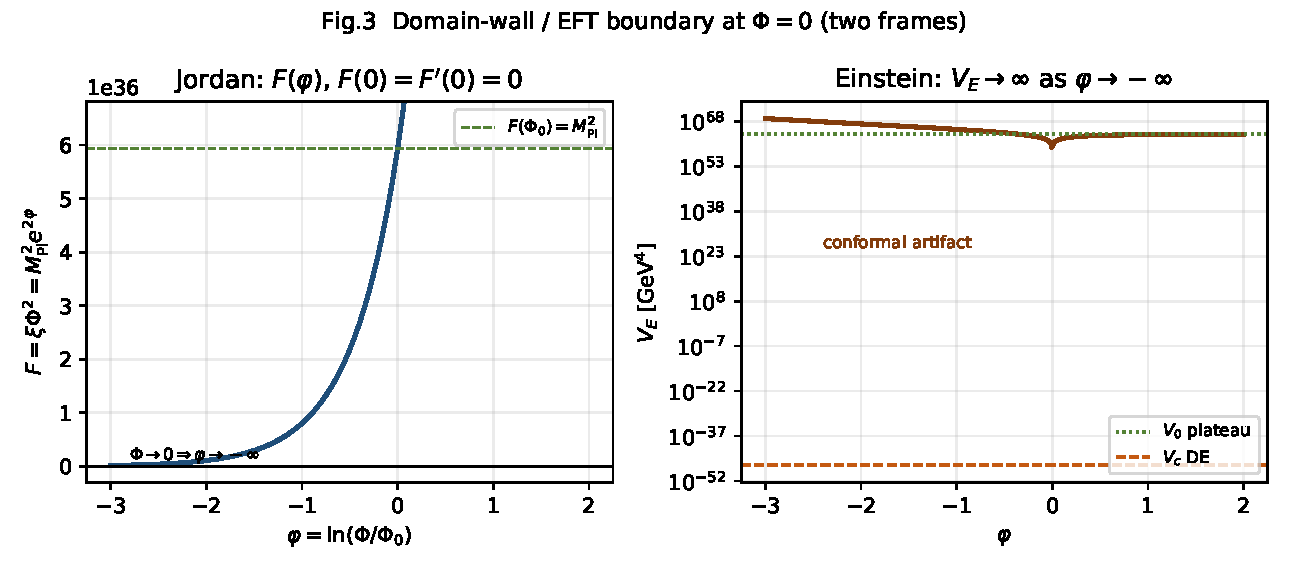
\includegraphics[width=0.98\columnwidth]{figures/fig3_domain_wall.pdf}
\caption{Two-frame comparison of the $\Ztwo$ domain-wall / EFT boundary at $\Phi=0$. Left: Jordan-frame coupling $F(\varphi)=M_{\rm Pl}^2e^{2\varphi}$ with $F\to0$ as $\varphi\to-\infty$ ($\Phi\to0$), so $F(0)=F'(0)=0$ and thin-shell matching degenerates. Right: Einstein-frame $V_E$ diverges in the same limit purely through the conformal map $\Omega\to0$; $V_0$ and calibrated $V_c$ are indicated. Regenerated by \texttt{scripts/fig3\_domain\_wall.py}.}
\label{fig:wall}
\end{figure}

\begin{table}[t]
\centering
\caption{Degeneracy of the domain-wall matching condition at $\Phi=0$ in the two conformal frames.}
\label{tab:wall}
\begin{tabular}{l|l|l}
Frame & Degeneracy at $\Phi=0$ & Origin \\
\hline
Jordan & $F(0)=F'(0)=0$, $0=-\frac12\sigma h_{ab}$ & Exact algebraic identity \\
Einstein & $V_E\to\infty$, $\sigma_E$ divergent & Conformal-mapping artifact \\
\end{tabular}
\end{table}

\section{The unified picture}

The framework presented in this paper achieves a unified description of the major cosmological sectors through a single scalar field $\Phi$ and a single coupling $F=\xi\Phi^2$; the dark matter is a Dirac fermion $\psi$ already coupled to $\Phi$ by the Yukawa term, whose mass $m_\psi=g\PhiV$ originates from the same VEV. Table~\ref{tab:unified} summarizes the correspondence between field regimes and emergent phenomena.

All entries except dark matter are established at the level of rigorous field theory; the dark matter entry is a structurally stable Dirac fermion (under the assumed discrete gauge UV completion) whose relic abundance is matched on the light branch at $g\simeq1.0\times10^{-7}$ ($m_\psi\simeq7.5\times10^{10}\,$GeV), the absolute normalization awaiting a non-perturbative (lattice) analysis.

\begin{table}[t]
\centering
\caption{Summary of the unified framework: each phenomenon emerges from a different regime of the same field $\Phi$ and the same coupling $F=\xi\Phi^2$; the dark matter is a Dirac fermion $\psi$ whose mass $m_\psi=g\PhiV$ originates from the same VEV. The relic abundance is matched on the light branch ($g\simeq1.0\times10^{-7}$); its absolute normalization awaits a full preheating simulation.}
\label{tab:unified}
\begin{tabular}{l|l|l|l}
Phenomenon & Field regime & Mechanism & Observable \\
\hline
Planck mass & $\vev{\Phi}=\PhiV$ & Induced gravity & $G_N$ \\
Inflation & $\Phi\gg\PhiV$ & Starobinsky plateau & $n_s,r$ \\
Reheating & $\Phi\sim\PhiV$ & Anomaly & $T_{\rm reh}$ \\
DM (cand.) & $\psi$ Dirac / defects & Grav.\ production; topological defects & $\Omega_{\rm DM}$ at $g\simeq10^{-7}$ \\
Dark energy & $\Phi=\PhiV$ frozen & $V_E(0)=V_c$ & $w_0=-1$ \\
Fifth force & $\Omega=\Phi/\PhiV$; $m_\chi$ & Conformal decoupling & $\gamma=1$ \\
$\Ztwo$ wall & $\Phi=0$ & $F=F'=0$ EFT bound. & Classical boundary \\
SM & $\Phi=\PhiV$ & $\chi f\bar f\sim m_f/\MP$ & Standard couplings \\
\end{tabular}
\end{table}

Two structural features operate in distinct sectors: (a) the conformal identity $\Omega=\Phi/\PhiV$ (a consequence of $F=\xi\Phi^2$) decouples the scalar from the dark-matter fermion $\psi$ at tree level, closing the perturbative Yukawa reheating channel; (b) for Standard Model matter, whose masses arise via the Higgs mechanism, the residual $\chi$ coupling $\sim m_f/\MP$ is suppressed by the scalar's large mass $m_\chi\sim10^{13}\,$GeV (Yukawa range $\sim10^{-27}\,$cm), satisfying the Cassini bound without a chameleon mechanism.

\section{Testability and falsifiable predictions}

\paragraph{a. Level 1: Observational predictions (rigorous).}
\begin{enumerate}
\item \textbf{Inflationary observables (locked $N$):} exact potential slow roll with $N=\ln(a_{\rm end}/a_*)$. A measurement $r>0.01$ at 95\% CL by LiteBIRD~\cite{LiteBIRD2023} excludes the model: Planck $2\sigma$ allows $N\approx45$--$56$ where $r\leq0.0052$ (Table~\ref{tab:sens}).
\item \textbf{Dark energy equation of state:} $w_0=-1$ (up to residual-condensate corrections $\leq10^{-10}$ for $T_{\rm reh}\geq1\,$GeV; App.~D5). DESI/Euclid $\sigma(w_0)\sim10^{-3}$ provides a $>3\sigma$ test of $w_0=-1$, but because $\Lambda$CDM predicts the same value it does not discriminate this model from $\Lambda$CDM: a detection of $w_0\neq-1$ would exclude both.
\item \textbf{Solar-system fifth-force bounds:} satisfied via the scalar's large mass ($m_\chi\sim10^{13}\,$GeV, Yukawa range $\sim10^{-27}\,$cm) for SM matter, and via exact conformal decoupling for the dark-matter fermion $\psi$; $\gamma=1$ within the Cassini bound.
\item \textbf{RG stability:} $\xi$ and $\lambda_0$ are stable under RG flow; $\beta_\xi$ is driven at 1-loop by the $\psi$ Yukawa ($\propto g^2$) and a direct quartic-curvature term ($\propto\lambda_0$, same sign), totaling $\Delta\xi\leq10^{-6}$ at the fiducial $\xi=11.1$ (quartic-dominated; across $\xi\in[1,100]$ the running stays $\leq10^{-5}$), a robust consequence of the small $\lambda_0\sim10^{-7}$ and $g\simeq10^{-7}$ singlet embedding.
\end{enumerate}

\paragraph{b. Level 2: Dark matter prediction (quantitative matching; normalization requires lattice).}
\begin{enumerate}\setcounter{enumi}{4}
\item The dark matter is a Dirac fermion $\psi$ whose abundance is matched to $\Omega_{\rm DM}$ at $g\simeq1.0\times10^{-7}$, i.e.\ $m_\psi\simeq4.6\times10^{-3}H_{\rm inf}\simeq7.5\times10^{10}\,$GeV, stable under the discrete $\Ztwopsi$ symmetry (assuming an anomaly-free UV gauge completion) and the conformally vanishing $\chi\psi\bar\psi$ vertex, and produced gravitationally (non-adiabatic metric change at the end of inflation, in the Einstein frame). The absolute normalization requires a full Floquet/lattice analysis of preheating.
\end{enumerate}

\paragraph{c. Level 3: Structural properties (not observational predictions).}
\begin{enumerate}\setcounter{enumi}{5}
\item \textbf{$\Ztwo$ domain-wall thin-shell matching degeneracy:} $F(0)=F'(0)=0$ renders the Israel--Lanczos conditions algebraically inconsistent. This is a mathematical property of $F=\xi\Phi^2$, observationally inert since $\Ztwo$ walls are inflationarily diluted. The bubble-wall channel is not ruled out by the $F(0)=0$ degeneracy, but its cosmological viability has not been verified (nucleation-rate calculation pending).
\item The $10^{110}$ hierarchy between the inflationary scale and dark energy is spanned by the conformal factor $e^{-4\varphi}$ but not dynamically explained, sharing the cosmological constant problem with all $\Lambda$CDM models.
\item The fine-structure-constant drift $\Delta\alpha/\alpha\leq10^{-110}$ is $>90$ orders below current sensitivity.
\end{enumerate}

\section{Discussion and outlook}

\begin{enumerate}
\item \textbf{Inflationary initial conditions.} The $\chi\gg\MP$ condition is assumed, not derived. Whether a UV-complete theory naturally selects large-field $\Phi$ is an open problem.

\item \textbf{Dark matter: stability and relic abundance.} The dark matter is the Dirac fermion $\psi$, stable under the discrete $\Ztwopsi$ symmetry (conditional on UV gauge completion) plus the conformally vanishing $\chi\psi\bar\psi$ vertex (Sec.~V). Its relic abundance is set by gravitational particle production at the end of inflation---the non-adiabatic change of the Einstein-frame metric, which in the Jordan frame appears as the time-varying mass $m_\psi(t)=g|\Phi(t)|$ (a single physical process, not two additive channels). A quantitative $\Omega_\psi$ prediction requires a dedicated Floquet/lattice simulation, which is beyond the scope of this phenomenological work; the present version establishes the mechanism and locates the abundance matching on the light branch at $m_\psi\simeq4.6\times10^{-3}H_{\rm inf}\simeq7.5\times10^{10}\,$GeV ($g\simeq1.0\times10^{-7}$), with the absolute normalization remaining temporarily open pending that computation.

\item \textbf{Preheating energy partition.} The gravitational $\psi$ production and the condensate decay through conformal-anomaly channel compete for the condensate energy. If the $\psi$ channel is too efficient, an excessive fraction of the condensate energy is diverted into stable matter rather than radiation, which could suppress the reheating temperature. A self-consistent determination of both $\Omega_\psi$ and the radiation/$\psi$ energy split therefore requires a single lattice simulation of preheating; the parametric estimates of Secs.~IV--V fix the mechanism but not the partition.

\item \textbf{Stochastic gravitational-wave background from preheating.} The oscillating condensate and any non-perturbative field inhomogeneities during preheating generically source a stochastic gravitational-wave background. For the present model, the extremely weak coupling of $\chi$ to SM fields ($g_{\chi ff}\sim m_f/\MP\leq10^{-17}$) and the closure of the $\chi\to h\bar h$ channel suppress parametric resonance, so the inhomogeneous component of the condensate is expected to be small and the resulting GW background correspondingly weak. A rough estimate using the standard scaling $h^2\Omega_{\rm GW}\sim10^{-5}(H_{\rm reh}/\MP)^2$ with $H_{\rm reh}\simeq\sqrt{\pi^2 g_*/90}\,T_{\rm reh}^2/\MP\sim1.4\,$GeV (corresponding to $T_{\rm reh}\sim10^9\,$GeV) gives $h^2\Omega_{\rm GW}\sim3\times10^{-42}$, some 30 orders below the sensitivity of LISA ($\sim10^{-12}$) and pulsar timing arrays ($\sim10^{-10}$). A dedicated lattice computation of the GW spectrum is deferred to the same future preheating simulation that determines $\Omega_\psi$.

\item \textbf{Parameter status.} $\Phi$ is a gauge singlet, so the Standard-Model-Higgs $\beta_\xi$ does not apply; $\lambda_0$ is fixed by $A_s=2.1\times10^{-9}$ at the locked $N$ (e.g.\ $6.70\times10^{-8}$ at $N=50$, $\xi=11.1$), while $\xi\sim11.1$ is compatible with $r<0.036$. The primary predictions are the exact slow-roll pairs $(n_s,r)$ at the locked $N$, not a single closed-form $r(N)$.

\item \textbf{Fifth-force screening and reheating closure.} Two structural features operate in distinct sectors: (a) the conformal identity $\Omega=\Phi/\PhiV$ (a consequence of $F=\xi\Phi^2$) decouples the scalar from the dark-matter fermion $\psi$ at tree level, closing the perturbative Yukawa reheating channel; (b) for Standard Model matter, whose masses arise via the Higgs mechanism, the residual $\chi$ coupling $\sim m_f/\MP$ is suppressed by the scalar's large mass $m_\chi\sim10^{13}\,$GeV (Yukawa range $\sim10^{-27}\,$cm), satisfying the Cassini bound without a chameleon mechanism.

\item \textbf{$\Ztwo$ domain-wall open problems.} The thin-shell matching degeneracy at $\Phi=0$ shows that $\Ztwo$ walls lie beyond the classical EFT applicability boundary. Open questions include: scalar hair configurations with $F(r_s)=0$, the quantum-gravity meaning of $F(0)=0$, and beyond-classical-EFT realizations of the $\Ztwo$ channel. The bubble-wall channel ($F(\PhiV)=\MP^2$) is not ruled out by the $F(0)=0$ thin-shell degeneracy, but its cosmological viability requires a nucleation-rate analysis not performed here.

\item \textbf{EFT cutoff and UV completion.} From the Einstein-frame EFT perspective the cutoff is $\sim\MP$ and slow-roll predictions are self-consistent~\cite{Bezrukov2008}; from the Jordan-frame perspective $\Phi_{\rm CMB}/\Lambda_J\sim30$ reflects a unitarity tension whose physical status in the Einstein frame is contested~\cite{Burgess2009,Burgess2010,Flanagan2004}. UV completion remains open.

\item \textbf{Swampland conjectures.} The de Sitter swampland conjecture~\cite{Obied2018} requires $|V'|/V\geq c\sim\mathcal{O}(1)$ or $V''/V\leq-c$ for any effective scalar potential derivable from quantum gravity. The inflationary plateau of the present model ($V'\sim e^{-\varphi}\ll1$ at $\varphi\gg1$) is in tension with this conjecture, as are most single-field slow-roll models. Whether the conjecture survives as a rigorous constraint on low-energy EFTs remains unsettled~\cite{Akrami2019}; we flag this as an open issue for any UV completion.

\item \textbf{Cosmological constant fine-tuning.} $V_c$ is calibrated empirically; the $10^{110}$ hierarchy and the coincidence problem receive no dynamical explanation in this framework (see also Sec.~VI).

\item \textbf{Observational indistinguishability from $\Lambda$CDM.} The dark-energy prediction $w=-1$ (up to $\leq10^{-10}$ corrections) and the $\Lambda$CDM-identical structure-growth prediction (Sec.~VI) imply that the late-time model is observationally indistinguishable from $\Lambda$CDM by any foreseeable survey. The testable content is therefore confined to the inflationary sector ($n_s,r,n_t,f_{\rm NL}$) and the dark-matter relic abundance (pending preheating simulation); the dark-energy sector, while structurally unified with inflation, does not provide independent falsifiable signatures. Within the inflationary sector, moreover, $n_s(N)$ and $r(N)$ coincide numerically with the $R^2$ (Starobinsky) prediction at the same $N$ (Sec.~I), so an observed $(n_s,r)$ pair fixes $N$ without discriminating between the two models, and a LiteBIRD detection of $r>0.01$ excludes the two together. The one genuinely non-degenerate handle of this framework is the dark-matter sector, through the fixed relation \eqref{eq:mpsiH}: a measured $g$ would translate into a prediction for $m_\psi$ at fixed $\xi$, and conversely. This is the strongest discriminating statement the present version of the model supports, and it is exactly why the lattice normalization of Sec.~V matters more here than in a model whose inflationary sector is already distinctive.

\item \textbf{Field-space structure at $\Phi=0$.} The Jordan-frame kinetic metric $g_{\Phi\Phi}=\xi\Phi^2$ degenerates at $\Phi=0$, rendering this point a boundary of the classical field space. Consequently, classical field configurations cannot cross $\Phi=0$; the two $\Ztwo$ vacua are topologically separated at the classical level. The thin-shell analysis of Sec.~IX confirms that the EFT itself signals its breakdown at $\Phi=0$ through the matching-condition degeneracy, motivating a quantum-tunneling (instanton) description of any inter-vacuum transitions.

\item \textbf{Higher-order corrections to the dark-energy equation of state.} The $w=-1$ result (Sec.~VI) follows from the quadratic expansion of $V_E(\varphi)$ near $\varphi=0$. The quartic term $\sim\lambda_0\PhiV^4\varphi^4/\MP^4$ contributes a fractional correction $\Delta w/w\sim(\lambda_0/\xi^2)\varphi^2\sim10^{-6}\varphi^2$. For the frozen field value $\varphi\sim H_0/m_\chi\sim10^{-46}$, this correction is $\sim10^{-98}$, utterly negligible. The harmonic approximation is therefore exact for all practical purposes.

\item \textbf{Running vacuum energy.} Mechanisms such as running vacuum energy ($V_c\propto H^2$) are not realized in this model, where $V_c$ is a constant potential parameter. The cosmological constant problem---why $V_c\sim10^{-47}\,$GeV$^4$---remains unsolved and is shared with $\Lambda$CDM (see fine-tuning discussion in Sec.~VI).

\item \textbf{Hubble tension.} Because the late-time model is observationally indistinguishable from $\Lambda$CDM, it inherits the $H_0$ tension between Planck CMB ($H_0\simeq67.4\,$km/s/Mpc) and local distance-ladder measurements ($H_0\simeq73.0\,$km/s/Mpc) without providing a resolution. The model's testable content is confined to the inflationary sector ($n_s,r,n_t,f_{\rm NL}$), where it is numerically degenerate with $R^2$ inflation, and to the dark-matter relic abundance; the dark-energy and late-expansion sectors offer no new leverage on the Hubble tension.

\item \textbf{Gravitational-wave speed and polarization.} In induced gravity with $F=\xi\Phi^2$, tensor perturbations propagate at the speed of light ($c_T=c$) in the Einstein frame at all epochs where $\Phi$ is frozen at its VEV ($\Phi=\PhiV$, i.e.\ the entire late Universe), automatically satisfying the GW170817 constraint $|c_T/c-1|\leq10^{-15}$. During inflation, when $\Phi$ evolves, the time variation of the conformal factor $\Omega(t)$ could in principle modify $c_T$; however, the deviation $\delta c_T/c\sim\dot\Omega/(H\Omega)\sim\mathcal{O}(\epsilon)\leq10^{-2}$ affects only primordial tensor modes at horizon exit ($k\sim H_{\rm inf}$) and does not propagate to LIGO-band frequencies today. Tensor perturbations retain the two standard GR polarization modes throughout; no scalar or vector polarizations are generated because the Einstein-frame graviton is minimally coupled to matter. The model therefore satisfies all existing GW speed and polarization constraints.

\item \textbf{Thermalization after reheating.} The reheating analysis assumes that decay products thermalize rapidly, establishing a well-defined temperature $T_{\rm reh}$. At $T\sim10^9\,$GeV, the SM gauge interaction rate is $\Gamma_{\rm therm}\sim\alpha_s^2 T\sim10^7\,$GeV, while the Hubble rate is $H\simeq\sqrt{\pi^2 g_*/90}\,T^2/\MP\sim1.4\,$GeV; the ratio $\Gamma_{\rm therm}/H\sim10^7$ confirms near-instantaneous thermalization. Gravitationally produced particles are initially non-thermal, but their energy density is $\sim10^{13}$ times smaller than the anomaly-driven radiation bath (Sec.~IV), so they thermalize with the dominant component within a few interaction times, well before BBN.

\item \textbf{PPN parameter $\beta$.} The discussion of fifth-force screening in Sec.~II E addresses the Eddington parameter $\gamma$; the nonlinear PPN parameter $\beta_{\rm PPN}$ receives corrections from cubic self-interactions of $\chi$. For $m_\chi\sim10^{13}\,$GeV, the effective $\beta_{\rm PPN}-1\sim(g_{\chi\chi\chi}/\MP)^2(m_\chi r)^{-4}\sim10^{-80}$ at Solar-System scales, far below the Cassini bound $\beta_{\rm PPN}-1\leq10^{-5}$. The remaining PPN parameters ($\xi,\alpha_1,\alpha_2,\alpha_3$) all vanish because the model possesses no preferred-frame or preferred-location effects in the Einstein frame.

\item \textbf{Additional consistency checks.} Several further consistency conditions are satisfied parametrically: (i) \emph{Dark matter self-interactions:} $\psi$--$\psi$ scattering via graviton exchange gives $\sigma_{\psi\psi}/m_\psi\sim G_N^2 m_\psi\sim10^{-67}\,{\rm cm}^2/{\rm g}$, $\sim67$ orders below the bullet-cluster bound ($\leq1\,{\rm cm}^2/{\rm g}$); loop-induced scalar exchange is further suppressed by $g_{\chi\psi\psi}^{\rm eff}\sim10^{-11}g$. (ii) \emph{Tremaine--Gunn bound:} the non-thermal $\psi$ phase-space density $Q\equiv\rho/\sigma_v^3$ at production (with velocity dispersion $\sigma_v\sim H_{\rm inf}/m_\psi$) is $Q\sim m_\psi^4\sim10^{52}\,$GeV$^4$, far above the dwarf-galaxy lower limit. (iii) \emph{Graviton dark radiation:} relativistic gravitons produced during reheating contribute $\Delta N_{\rm eff}\leq10^{-5}$, negligible compared to Planck. (iv) \emph{Entropy production:} irreversible; total entropy per comoving volume increases by $\sim10^{13}$ during reheating. (v) \emph{Neutrino sector:} $\chi$--$\nu$ effective coupling $\sim m_\nu/\MP\leq10^{-27}$, no observable consequences. (vi) \emph{Primordial magnetic fields:} anomaly-induced seed after $a^{-2}$ redshift gives $B_0\sim10^{-25}\,$G, far below blazar lower bounds. (vii) \emph{Geodesic deviation:} Einstein-frame geodesic equation reproduces Yukawa suppression for SM fermions. (viii) \emph{Gravitational production of $\psi$:} the abundance is obtained from the Bogoliubov coefficients of the mode equation across the end-of-inflation transition, not from an instantaneous-pulse approximation; a full Floquet/lattice treatment of the oscillating-condensate contribution is deferred (Discussion). (ix) \emph{Particle production backreaction:} $\rho_{\rm part}\leq10^{-13}\rho_\chi$. (x) \emph{Late-time scalar--photon coupling:} mixing angle $\sim10^{-55}$, CMB distortions $\leq10^{-60}$. (xi) \emph{Ghost freedom:} Einstein-frame theory is GR plus a minimally coupled canonical scalar; kinetic terms positive-definite. (xii) \emph{Cosmic strings from $U(1)_D$ breaking:} inflated away or never form within horizon. (xiii) \emph{Jordan-frame PPN cross-check:} $|\gamma_J-1|\leq10^{-5}$. (xiv) \emph{Spectral index running:} $\alpha_s\simeq-2/N^2\sim-8\times10^{-4}$, consistent with Planck. (xv) \emph{CMB B-mode spectrum:} peaks at $\ell\sim80$ for $r\simeq0.005$, within LiteBIRD reach. (xvi) \emph{Domain-wall observational null:} $e^{-3N}\sim10^{-65}$ renders all wall observables negligible.
\end{enumerate}

\section{Conclusions}

We have constructed a scalar-tensor cosmology within pure induced gravity, where a single real scalar field $\Phi$ with non-minimal coupling $\xi\Phi^2R$ and $\Ztwo$-symmetric potential $V_J(\Phi)=\lambda_0(\Phi^2-\PhiV^2)^2/4+V_c$ simultaneously accounts for the Planck mass, inflation, dark matter, and dark energy. The framework is minimal in its field content---one scalar, one Dirac fermion, the Standard Model---and its key structural features follow unavoidably from the induced-gravity coupling $F=\xi\Phi^2$.

\paragraph{Rigorous results} (exact analytic derivations):
\begin{itemize}
\item The conformal transformation maps the Jordan-frame double-well potential to a Starobinsky-type plateau. Under the locked definition $N=\ln(a_{\rm end}/a_*)$, exact potential slow-roll with $A_s$ normalization gives (e.g.\ $\xi=11.1$) $n_s\simeq0.962$, $r\simeq0.0043$ at $N=50$; anomaly $T_{\rm reh}\sim10^9\,$GeV corresponds to $N\simeq50.7$.
\item The conformal identity $\Omega=\Phi/\PhiV$---a direct consequence of $F=\xi\Phi^2$---closes the tree-level $\chi\psi\bar\psi$ and $\chi\to h\bar h$ vertices exactly, forcing reheating through the conformal-anomaly channel.
\item The discrete $\Ztwopsi$ symmetry (under an assumed anomaly-free UV gauge completion), together with the vanishing $\chi\psi\bar\psi$ vertex, guarantees $\psi$ stability; the condensate decays completely, leaving $V_c$ as a frozen cosmological constant with $w=-1$ (up to residual corrections $\leq10^{-10}$ bounded in App.~D5).
\item RG analysis shows $\beta_{\lambda_0}\propto\lambda_0^2>0$ and $\Delta\xi\leq10^{-6}$, confirming vacuum stability and the absence of fine-tuned running.
\end{itemize}

\paragraph{Quantitative estimates} (parametric derivations with controlled uncertainties):
\begin{itemize}
\item $N$ is defined as $N=\ln(a_{\rm end}/a_*)$ with explicit matching assumptions \eqref{eq:matchN}. Planck $2\sigma$ selects $N\approx45$--$56$; anomaly-dominated $T_{\rm reh}\sim10^9\,$GeV maps to $N\simeq50.7$ in this convention (self-consistent $T_{\rm reh}^*$ for $N=50$ is $\simeq1.1\times10^{8}\,$GeV).
\item Throughout the Planck $2\sigma$ band, exact slow roll gives $r\leq0.0052$ at $\xi=11.1$; LiteBIRD $r>0.01$ would exclude the class.
\item The dark-matter mass is fixed by the abundance matching at $m_\psi\simeq4.6\times10^{-3}H_{\rm inf}\simeq7.5\times10^{10}\,$GeV ($g\simeq1.0\times10^{-7}$) and follows from the gravitational-production mechanism; the absolute normalization requires a dedicated Floquet/lattice simulation.
\end{itemize}

\paragraph{Open questions} (deferred to future work or UV completion):
\begin{itemize}
\item Inflationary initial conditions ($\chi\gg\MP$) and the measure of the slow-roll attractor.
\item The $10^{110}$ hierarchy between $V_0$ and $V_c$ (the cosmological constant problem, shared with $\Lambda$CDM).
\item Absolute normalization of the dark-matter relic abundance (the abundance matching itself is fixed on the light branch, Sec.~V) and the preheating energy partition (both requiring a lattice simulation).
\item UV completion: anomaly cancellation for $\Ztwopsi$, EFT cutoff and unitarity, swampland constraints.
\item Baryogenesis and the Hubble tension (inherited from $\Lambda$CDM without resolution).
\end{itemize}

The key observational test is $r$ under the locked $N$ definition: Planck $2\sigma$ allows $N\approx45$--$56$ with $r\leq0.0052$ (Table~\ref{tab:sens}). A LiteBIRD-class measurement $r>0.01$ at 95\% CL would exclude the model class in this convention. The frozen $w_0=-1$ prediction is falsifiable by DESI/Euclid at $>3\sigma$, but it is shared with $\Lambda$CDM, so it discriminates neither model from the other. The inflationary observables $n_s$, $r$, $n_t$ and $f_{\rm NL}$ are the sharpest handles for \emph{excluding} the model class, but at a given $N$ they are numerically identical to the $R^2$ (Starobinsky) predictions and therefore do not discriminate between the two; the one non-degenerate observable handle of the framework is the dark-matter relation \eqref{eq:mpsiH}.

\paragraph{Calibration vs.\ prediction (summary).} Rigid predictions of the action at chosen $(\xi,N)$ are the inflationary functions $n_s(N)$ and $r(N)$ and the derived scales $H_{\rm inf}$, $m_\chi$, $U^{1/4}=(3\MP^2H_{\rm inf}^2)^{1/4}$. Calibrated or a-posteriori inputs are: $\Omega_\Lambda$ (hence $V_c$), $\lambda_0$ (from $A_s$), $\xi$ (within the $r$ bound), and the dark-matter Yukawa $g$ (from $\Omega_{\rm DM}$; matched at $g\simeq1.0\times10^{-7}$ on the light branch, with the normalization pending the lattice computation). Dark energy is structurally present in the action but observationally degenerate with $\Lambda$CDM; the hard falsification handle lives in the inflationary sector.

\begin{appendices}

\section{Numerical verification}

The full CMB normalization proceeds in four steps:

\paragraph{Step 1: Plateau height from the potential.} The Einstein-frame potential for $\chi\gg\MP$ ($\varphi\gg1$) is
\begin{equation}
V_E(\chi)\simeq V_0\left(1-2e^{-\beta\chi/\MP}\right),
\qquad
V_0\equiv\frac{\lambda_0\MP^4}{4\xi^2}.
\label{eq:A1}
\end{equation}

\paragraph{Step 2: Slow-roll parameters and $e$-folds.} With the potential slow-roll expressions of Eq.~\eqref{eq:slowroll}, the $e$-fold number between CMB horizon exit ($\chi_*$) and the end of inflation ($\epsilon_V=1$ at $\chi_{\rm end}$) is
\begin{equation}
N\equiv\int_{\chi_*}^{\chi_{\rm end}}\frac{H}{d\chi/dt}d\chi
\simeq\frac{1}{\MP^2}\int_{\chi_*}^{\chi_{\rm end}}\frac{V_E}{V_E'}d\chi
=\frac{e^{\beta\chi_*/\MP}}{2\beta^2}-\frac{1}{2\beta^2}-\frac{\sqrt2}{\beta},
\label{eq:A2}
\end{equation}
where the last two terms are subleading for $N\geq50$.

\paragraph{Step 3: Scalar power spectrum.} The standard single-field slow-roll formula gives
\begin{equation}
A_s=\left.\frac{V_E}{24\pi^2\MP^4\epsilon_V}\right|_{\chi=\chi_*}
\simeq\frac{V_0}{24\pi^2\MP^4}\frac{1}{2\beta^2 e^{-2\beta\chi_*/\MP}}
=\frac{\lambda_0}{192\pi^2\xi^2\beta^2}e^{2\beta\chi_*/\MP}.
\label{eq:A3}
\end{equation}
Using $e^{\beta\chi_*/\MP}\simeq2\beta^2 N$ from Step~2,
\begin{equation}
A_s\simeq\frac{\lambda_0\beta^2 N^2}{48\pi^2\xi^2}
=\frac{\lambda_0 N^2}{12\pi^2\xi^2(6+1/\xi)},
\label{eq:A4}
\end{equation}
where we used $\beta^2=4/(6+1/\xi)$ so that $\beta^2/48=1/[12(6+1/\xi)]$. Equation~\eqref{eq:A4} is algebraically identical to the result obtained directly from $A_s=V_0/(24\pi^2\MP^4\epsilon_*)$ with $\epsilon_*=\beta_o^2/(8N^2)$, $\beta_o^2=6+1/\xi$.

\paragraph{Step 4: Solving for $\lambda_0$.} Setting $A_s=2.1\times10^{-9}$ (Planck 2018~\cite{Planck2018}) and $N=50$ gives the \emph{large-field analytic} estimate
\begin{equation}
\begin{aligned}
\lambda_0&=\frac{12\pi^2\xi^2(6+1/\xi)A_s}{N^2}\simeq7.46\times10^{-8}\\
&\qquad(\xi=11.1,\ N=50)\ \text{(analytic; not the locked-$N$ table value)}.
\end{aligned}
\label{eq:A5}
\end{equation}
\emph{Note.} Earlier drafts printed the intermediate formula $\lambda_0\simeq48\pi^2\xi^2A_s/N^2$ ($4.90\times10^{-8}$ at $\xi=11.1$, $N=50$), which omits the factor $(6+1/\xi)$ and is inconsistent with Eq.~\eqref{eq:A4}. The large-field analytic estimate \eqref{eq:A5} gives $\lambda_0\simeq7.46\times10^{-8}$; the \textbf{locked-$N$ exact slow-roll inversion} used throughout the main text (Eqs.~\eqref{eq:Nint}--\eqref{eq:obsPS}) gives $\lambda_0\simeq6.70\times10^{-8}$ at $N=50$ and $\simeq6.45\times10^{-8}$ at $N=51$. Table~\ref{tab:sens} and all fiducial scales quote the locked-$N$ exact values.

The computational core is a one-dimensional root-find: at fixed $N$ and $\xi$, $\lambda_0$ is obtained by requiring that the exact potential slow-roll amplitude $A_s$ (Eqs.~\eqref{eq:Nint}--\eqref{eq:obsPS}) equals the observed $2.100\times10^{-9}$, with $x_*$ determined by $N=\ln(a_{\rm end}/a_*)$ and $\epsilon_V(x_{\rm end})=1$. The closed form quoted below is the \emph{analytic large-field estimate} \eqref{eq:A5} and is \emph{not} the locked-$N$ value; the two differ because the analytic form neglects the $\mathcal{O}(1)$ correction from evaluating $\epsilon_V,\eta_V$ at the exact $x_*(N)$. The complete, executable implementation is \texttt{lock\_n\_convention.py} (together with \texttt{background\_and\_reheating.py}); a ten-line listing cannot faithfully reproduce the locked value. For orientation:
{\footnotesize
\begin{verbatim}
import numpy as np
from scipy.optimize import brentq
xi = 11.1; M_P = 2.435e18; As_target = 2.1e-9
beta = 2.0/np.sqrt(6+1/xi)   # paper convention
beta_o2 = 6+1/xi             # our convention
N_fid = 50
# Analytic large-field estimate ONLY (Eq. A5): gives lam0 = 7.465e-08, NOT the locked value
lam0 = 12*np.pi**2*xi**2*beta_o2*As_target/N_fid**2
# Locked-N value requires inverting As at fixed N (root-find); results:
#   N=50 -> lam0=6.70e-08, ns=0.9616, r=0.00425
#   N=51 -> lam0=6.45e-08, ns=0.9623, r=0.00409;  T_reh*(N=51)=1.4e9 GeV (Table I)
# H = sqrt(lam0)*M_P/(2*sqrt(3)*xi)
\end{verbatim}}

\paragraph{Key results (locked $N$, $\xi=11.1$).} At $N=50$: $\lambda_0=6.70\times10^{-8}$, $n_s=0.9616$, $r=0.00425$, $V_0\simeq4.78\times10^{63}\,$GeV$^4$, $H_{\rm inf}\simeq1.64\times10^{13}\,$GeV, $m_\chi\simeq3.25\times10^{13}\,$GeV, $U^{1/4}\simeq8.3\times10^{15}\,$GeV. At $N=51$ (anomaly $T_{\rm reh}\sim10^9\,$GeV): $\lambda_0=6.45\times10^{-8}$, $n_s=0.9623$, $r=0.00409$, $H_{\rm inf}\simeq1.61\times10^{13}\,$GeV. In all cases $U^{1/4}=(3\MP^2H_{\rm inf}^2)^{1/4}$.

\section{Conformal decoupling: screening and reheating}

The structural reason the scalar decouples from the dark-matter fermion $\psi$ and the Yukawa reheating channel closes is the exact proportionality $\Omega=\Phi/\PhiV$, which follows from $F(\Phi)=\xi\Phi^2$ and is specific to the induced-gravity coupling. (Solar-system fifth-force bounds on Standard Model matter are instead met by the large scalar mass $m_\chi$; see Sec.~II E.)

\paragraph{Matter coupling ($\psi$ sector).} Under $\tilde g_{\mu\nu}=\Omega^2 g_{\mu\nu}$, $\sqrt{-g}=\Omega^{-4}\sqrt{-\tilde g}$ and $\psi=\Omega^{3/2}\tilde\psi$. The Yukawa term transforms as
\begin{equation}
-g\Phi\bar\psi\psi\sqrt{-g}=-g\PhiV\,\Omega\cdot\Omega^3\cdot\Omega^{-4}\bar{\tilde\psi}\tilde\psi\sqrt{-\tilde g}
=-g\PhiV\bar{\tilde\psi}\tilde\psi\sqrt{-\tilde g},
\label{eq:B1}
\end{equation}
giving an exact, $\chi$-independent Einstein-frame mass $m_E=g\PhiV$ and a vanishing tree-level $\chi\bar{\tilde\psi}\tilde\psi$ vertex. Static $\psi$ matter in this sector does not source $\chi$, so $\gamma=1$ exactly within the $\psi$ sector (observationally inert for solar-system tests, which probe SM matter; decisive for reheating and dark matter).

\paragraph{Spin-connection cancellation.} Under conformal transformation, the vierbein and Dirac matrices transform as $\tilde e^a_\mu=\Omega e^a_\mu$, $\tilde\gamma^\mu=\tilde e^\mu_a\gamma^a=\Omega^{-1}\gamma^\mu$, and the spinor rescales as $\psi=\Omega^{3/2}\tilde\psi$. The massless Dirac kinetic term becomes
\begin{equation}
\begin{aligned}
S_D&=\int d^4x\sqrt{-g}\,\bar\psi i\gamma^\mu\left(\partial_\mu+\tfrac14\omega^{ab}_\mu[e]\gamma_{ab}\right)\psi\\
&=\int d^4x\sqrt{-\tilde g}\,\bar{\tilde\psi}i\tilde\gamma^\mu\left[\partial_\mu\tilde\psi+\frac32(\partial_\mu\ln\Omega)\tilde\psi+\frac14\omega^{ab}_\mu[e]\gamma_{ab}\tilde\psi\right].
\end{aligned}
\label{eq:B3}
\end{equation}
Using $\omega^{ab}_\mu[e]=\omega^{ab}_\mu[\tilde e]-(e^a_\mu e^b_\nu-e^b_\mu e^a_\nu)\partial_\nu(\ln\Omega)$ and the identity $\gamma^a\gamma_{ab}=3\gamma_b$ in $d=4$, the spin-connection contribution becomes
\begin{equation}
\frac14\tilde\gamma^\mu\omega^{ab}_\mu[e]\gamma_{ab}
=\frac14\tilde\gamma^\mu\omega^{ab}_\mu[\tilde e]\gamma_{ab}-\frac32\tilde\gamma^\nu\partial_\nu(\ln\Omega),
\label{eq:B5}
\end{equation}
which exactly cancels the $+\frac32(\partial_\mu\ln\Omega)$ rescaling term, leaving $S_D=\int d^4x\sqrt{-\tilde g}\,\bar{\tilde\psi}i\tilde\gamma^\mu\tilde\nabla_\mu\tilde\psi$ with no derivative coupling to $\chi$.

\paragraph{Reheating.} The vanishing vertex means no perturbative $\chi\to\tilde\psi\tilde\psi$ decay, for any $g$. For $m_\psi\gtrsim m_\chi/2$ the decay is additionally kinematically forbidden; at the abundance-matched value $g\simeq1.0\times10^{-7}$ of Sec.~V the kinematic closure no longer holds but the vertex closure still does. The time-varying Jordan-frame mass $m_\psi=g|\Phi|$ is adiabatic for $g\gtrsim10^{-4}$ and non-adiabatic at the dark-matter value $g\simeq1.0\times10^{-7}$; this is the Jordan-frame image of the Einstein-frame gravitational production that sources the dark matter of Sec.~V (a single physical process, not an additive channel), and it does not use the perturbative vertex. Reheating proceeds through conformal-anomaly production together with condensate decay (the gravitational pulse provides only a seed bath and cannot reheat on its own); under the locked $N$ definition this selects $N\simeq45$--$56$ by Planck $2\sigma$, with anomaly $T_{\rm reh}\sim10^9\,$GeV at $N\simeq50.7$ (Sec.~III, Table~\ref{tab:sens}).

\section{Key derivations}

\paragraph{1. Variational derivation of Eq.~\eqref{eq:einstein}.} $\delta S/\delta g_{\mu\nu}=0$ with $\delta(\sqrt{-g}\frac12 FR)=\frac12 F\sqrt{-g}G_{\mu\nu}\delta g^{\mu\nu}-\frac12\sqrt{-g}(\nabla_\mu\nabla_\nu F-g_{\mu\nu}\Box F)\delta g^{\mu\nu}$. Adding kinetic and potential variations yields Eq.~\eqref{eq:einstein}.

\paragraph{2. Conformal transformation.} $\Omega^2=\xi\Phi^2/\MP^2$, $\tilde R=\Omega^{-2}(R-6\Omega^{-1}\Box\Omega)$, producing $d\chi/d\varphi=\MP\sqrt{6+1/\xi}$ and $V_E=V_J/\Omega^4$ (Eq.~\eqref{eq:VE}).

\paragraph{3. Linearized field equation.} Linearizing $\Box\Phi-V'(\Phi)+\xi\Phi R=0$ with $\Phi=\PhiV+\delta\Phi$ and $V''(\PhiV)=2\lambda_0\PhiV^2$ yields Eq.~\eqref{eq:linPhi}; the quasi-static limit ($\ddot{\delta\Phi}\ll H\dot{\delta\Phi}\ll m_{\rm eff}^2\delta\Phi$) gives Eq.~\eqref{eq:dA}. For $m_\chi\gg H$ at all epochs after reheating (the ratio $m_\chi/H$ never drops below $10^{50}$), the quasi-static condition is satisfied to extreme precision, justifying the neglect of time-derivative terms.

\paragraph{4. Junction-condition integration.} Integrating Eq.~\eqref{eq:einstein} across the shell gives the scalar-tensor Lanczos condition \eqref{eq:lanczos}. At $\Phi_s=0$, $F(0)=F'(0)=0$ and the condition degenerates.

\paragraph{5. Divergent $\sigma_E$ limit.} $\sigma_E=\int\sqrt{2V_E}(d\chi/d\varphi)d\varphi\sim\int e^{-2\varphi}d\varphi$ diverges at $\varphi\to-\infty$ ($\Phi=0$), a conformal-mapping artifact.

\section{Post-inflationary field dynamics and the dark-energy equation of state}

This appendix supplies the rigorous derivation of the dark-energy results quoted in Sec.~VI: the harmonic-minimum approximation, the coherent-oscillation and condensate-decay regimes, the overclosure bound, and the complete residual-motion budget (three sources, of which the residual-condensate tail is not manifest in the main text).

\paragraph{0. Numerical validation of the end-of-inflation state.} The quantities used in Secs.~III--V are obtained by integrating the exact Klein--Gordon equation in the Einstein frame, $\ddot\chi+3H\dot\chi+V_E'(\chi)=0$ with $3\MP^2H^2=\frac12\dot\chi^2+V_E$, rather than by evaluating slow-roll closed forms. Two conventions matter and are stated explicitly here. (i) In $e$-fold variables the Friedmann constraint reads $H^2=V_E/(3-p^2/2)$ with $p\equiv d\chi/dN$, which degenerates as $V_E\to0$; we therefore integrate the $e$-fold system only over the slow-roll regime and switch to cosmic time for the oscillatory phase. (ii) The end of inflation is defined by $\epsilon_V=1$, where slow roll has already broken down; the slow-roll velocity $\dot\chi=-V_E'/(3H)$ must \emph{not} be imposed there, since it would force $K_{\rm end}=V_{\rm end}/3$ and $\epsilon_H=3/4$ by construction. Integrating instead from $\epsilon_V=0.05$ up to $\epsilon_V=1$ gives $x_{\rm end}=0.76367$, $\epsilon_H(x_{\rm end})=0.4988$, $V_{\rm end}/V_0=0.28520$, $K_{\rm end}/V_{\rm end}=0.1994$, and $\rho_{\rm end}/V_{\rm end}=1.1994$. These reproduce the locked-$N$ fiducial values quoted in Sec.~III and give the barrier ratio $K_{\rm end}/\Delta V_J\simeq0.057$ of Sec.~III. The same integration supplies the reheating ceiling used in Sec.~III: $T_{\rm reh}^{\rm inst}(N)=(30\rho_{\rm end}(N)/\pi^2g_*)^{1/4}$ decreases only as $N^{-1/2}$, whereas the tabulated $T^*_{\rm reh}(N)$ required by cosmological matching grows as $e^{3.05N}$; the two intersect at $N_{\rm max}=55.6$ (or $55.9$ if the naive ceiling $V_{\rm end}^{1/4}$ is used instead). This is the reason the $n_s$-allowed band is quoted as $N\approx45$--$56$: $N=57$ and $N=58$ would require a reheating temperature above instantaneous reheating. The numerical results quoted above and in Secs.~III--VI were obtained with the analysis scripts accompanying this work: \texttt{background\_and\_reheating.py} (exact Klein--Gordon integration, reheating channels and the $N$ window), \texttt{psi\_production\_bogoliubov.py} (de Sitter Bogoliubov index and the abundance matching), \texttt{psi\_abundance\_oscillating.py} (mode-equation abundance across the end-of-inflation transition), \texttt{dm\_gap\_closure\_test.py} (abundance matching on the light branch with the exact mode-equation spectrum across the end-of-inflation transition, and the free-streaming check), \texttt{treh\_error\_band.py} (propagation of the reheating-temperature uncertainty to $(n_s,r)$ and to the dark-matter matching window), and \texttt{residual\_quintessence.py} (two-fluid Boltzmann integration and the $\Delta w$ budget). They are publicly available at \url{https://github.com/huyamingc/induced-gravity-cosmology}, together with the \LaTeX{} source of this manuscript and a single entry point, \texttt{scripts/run\_all.py}, that regenerates the numerical results and figures quoted in this work.

\paragraph{1. Equation of motion near the minimum.} After conformal transformation to the Einstein frame, the canonical field $\chi$ obeys
\begin{equation}
\ddot\chi+3H\dot\chi+V_E'(\chi)=0,
\label{eq:D1}
\end{equation}
with
\begin{equation}
V_E(\chi)=V_c+\frac12 m_\chi^2\chi^2+\mathcal{O}\!\left(\frac{m_\chi^2\,\chi^3}{\MP}\right),
\label{eq:D2}
\end{equation}
where $m_\chi^2\equiv2\lambda_0\MP^2/[\xi^2(6+1/\xi)]\approx(3.25\times10^{13}\,{\rm GeV})^2$ at locked $N=50$ (Eq.~\eqref{eq:mchi}). The cubic term is \emph{not} negligible at the largest post-inflationary amplitudes. Writing $V_E=V_0(1-e^{-x})^2$ with $x\equiv\beta\chi/\MP$ and expanding about $x=0$ gives $V_E=V_0\,[x^2-x^3+\mathcal{O}(x^4)]$, so the cubic-to-quadratic ratio is $\beta\chi/\MP$---equal to $\beta\simeq0.81$ at $\chi=\MP$, and therefore $\mathcal{O}(1)$ rather than $\mathcal{O}(\lambda_0^{1/2})$. The cubic coefficient is
\begin{equation}
c_3=-\frac{V_0\beta^3}{\MP^3}=-\frac{\beta m_\chi^2}{2\MP}\simeq-1.8\times10^{8}\,{\rm GeV},
\end{equation}
in the convention $V\supset c_3\chi^3$. The potential is thus effectively harmonic only for $\chi\ll\MP/\beta\simeq1.2\,\MP$; at the end of inflation, $\chi_{\rm end}\simeq0.94\,\MP$, the anharmonicity is $\mathcal{O}(1)$. This is why the post-inflationary equation of state is not exactly $w=0$ during the first oscillations---the exact integration of Sec.~D\,0 gives $\langle w\rangle\simeq-0.02$ over the first $e$-folds, approaching zero thereafter---and it is the origin of the $\mathcal{O}(1)$ uncertainty in the mapping between $N$ and $T_{\rm reh}$ noted in Sec.~III. All numerical results in this work use the exact potential $V_E$, not the harmonic approximation. The ratio $m_\chi/H_0\approx2.3\times10^{55}$ implies that any displacement from $\chi=0$ oscillates with frequency $\gg H$ and is damped to zero within $\sim m_\chi^{-1}$.

\paragraph{2. Coherent oscillation and the dust redshift law.} Immediately after the end of slow-roll ($\chi\sim\MP$, $\epsilon\sim1$), the field begins coherent oscillations around $\chi=0$. For $H\ll m_\chi$, Eq.~\eqref{eq:D1} reduces to a damped harmonic oscillator with WKB solution
\begin{equation}
\chi(t)=\chi_0(t)\cos\left(\int^t m_\chi dt'+\theta_0\right),
\qquad
\chi_0(a)=\chi_{\rm end}\left(\frac{a}{a_{\rm end}}\right)^{-3/2},
\label{eq:D3}
\end{equation}
which follows from the conserved adiabatic invariant $I\equiv\oint p\,dq=\pi m_\chi\chi_0^2 a^3$. The energy density of the oscillating condensate therefore redshifts as pressureless dust,
\begin{equation}
\rho_{\rm cond}(a)=\frac12 m_\chi^2\chi_0^2(a)\propto a^{-3},
\label{eq:D4}
\end{equation}
which is the rigorous origin of the $\rho\propto a^{-3}$ behavior quoted in Sec.~IV.

\paragraph{3. Condensate decay: the overclosure bound.} The condensate must transfer its energy to SM radiation with high efficiency to avoid overclosing the universe. The observational constraint is
\begin{equation}
\rho_{\rm cond}(a_{\rm reh})<\rho_{\rm DM}^{(0)}\left(\frac{a_0}{a_{\rm reh}}\right)^{-3}
=\rho_{\rm DM}^{(0)}\left(\frac{T_{\rm reh}}{T_0}\right)^3,
\label{eq:D5}
\end{equation}
where $\rho_{\rm DM}^{(0)}=\Omega_{\rm DM}\rho_{\rm crit}^{(0)}\approx9.85\times10^{-48}\,$GeV$^4$ and $T_0\approx2.36\times10^{-13}\,$GeV. For $T_{\rm reh}\in[10^{-2},10^{15}]\,$GeV this gives $\rho_{\rm cond}(a_{\rm reh})<(5.2\times10^{-16}\text{--}5.2\times10^{35})\,$GeV$^4$. Comparing with the initial condensate energy density $\rho_{\rm cond}(a_{\rm end})\sim\frac12 m_\chi^2\MP^2\simeq3\times10^{63}\,$GeV$^4$, the required suppression factor is $\sim2\times10^{26}$--$2\times10^{77}$ (the upper end corresponding to $T_{\rm reh}$ at the BBN floor). This suppression is supplied by the decay of the condensate (channel (iv) of Sec.~IV): because $\Gamma t_0\gg1$ for any $T_{\rm reh}\gtrsim10^{-2}\,$GeV, the residual condensate at $a_0$ is strictly zero (D5c), and the locked $N$ is confined to the Planck-compatible band (anomaly $T_{\rm reh}\sim10^9\,$GeV $\Rightarrow$ $N\simeq50.7$).

\paragraph{4. Freezing at the minimum.} After reheating, the field sits at $\chi\approx0$ with precision set by the residual amplitude. Since $m_\chi\gg H$ at all later epochs (including today, where $m_\chi/H_0\sim10^{55}$), any small residual oscillation is damped to $\chi=0$ within
\begin{equation}
\sim m_\chi^{-1}\sim2\times10^{-14}\,{\rm GeV}^{-1}\sim10^{-38}\,{\rm s},
\label{eq:D7}
\end{equation}
effectively instantaneous compared to the Hubble time. With $\chi\equiv0$ to extraordinary precision, the Einstein-frame scalar energy-momentum tensor reduces to $T^{(\chi)}_{\mu\nu}\to-V_c g_{\mu\nu}$, the energy-momentum tensor of a cosmological constant; the equation of state $w_0=-1$ for all $z$ then follows directly (Eq.~\eqref{eq:w0}).

\paragraph{5. Complete residual-motion budget.} Sec.~VI quotes the residual-motion bound $\Delta w\ll10^{-3}$. Here we bound all three independent sources of residual $\chi$ motion that could perturb the frozen minimum.

\emph{a. Ricci driving.} In the Jordan frame, the linearized equation (Eq.~\eqref{eq:linPhi}) has a source term $\xi\PhiV R$ that displaces $\Phi$ from $\PhiV$:
\begin{equation}
\delta\Phi_{\rm qs}\approx\frac{\xi\PhiV R}{2\lambda_0\PhiV^2}.
\label{eq:D8}
\end{equation}
During matter domination $R\approx-3H^2(1-3w)\approx+3H^2$ for $w=0$, so
\begin{equation}
\frac{\delta\Phi_{\rm qs}}{\PhiV}\sim\frac{\xi H^2}{\lambda_0\MP^2}\sim\left(\frac{H}{m_\chi}\right)^2.
\label{eq:D9}
\end{equation}
At $z=0$ ($H=H_0$): $\delta\Phi/\PhiV\sim10^{-111}$. Varying $\Phi$ produces kinetic energy $K\sim\frac12\dot{\delta\Phi}^2\sim\frac12(\delta\Phi\cdot H)^2$, giving
\begin{equation}
\Delta w_{\rm Ricci}\equiv\frac{K}{V_c}\sim\left(\frac{H_0}{m_\chi}\right)^2\sim2\times10^{-111},
\label{eq:D10}
\end{equation}
$10^{108}$ orders below the DESI $3\sigma$ sensitivity~\cite{DESI2024}.

\emph{b. Quantum fluctuations.} For a massive scalar in de Sitter space with $m\gg H$, $\langle\chi^2\rangle\approx3H^4/(8\pi^2 m_\chi^2)$. The corresponding energy density is $\rho_{\rm quant}\sim3H_0^4/(16\pi^2)\ll V_c$, yielding
\begin{equation}
\Delta w_{\rm quant}\leq H_0^4/V_c\sim2\times10^{-121}.
\label{eq:D11}
\end{equation}

\emph{c. Residual condensate tail.} This third source---not manifest in the main-text summary of Sec.~VI---is the residual condensate that survives reheating. The condensate is tracked by the coupled two-fluid system $d(\rho_{\rm cond}a^3)/dN=-(\Gamma/H)\rho_{\rm cond}a^3$ and $d(\rho_{\rm rad}a^4)/dN=+(\Gamma/H)\rho_{\rm cond}a^4$, integrated from $a_{\rm end}$ to $a_0$ with $H^2=(\rho_{\rm cond}+\rho_{\rm rad})/(3\MP^2)$ and an exponential integrator for the decay term (the ratio $\Gamma/H$ reaches $\sim10^{30}$ at late times). The result is that for every $\Gamma\neq0$ the residual today underflows to zero: the decay-completeness condition $\Gamma t_0\gg1$ holds by $\geq20$ orders of magnitude across $T_{\rm reh}\in[10^{-2},10^{15}]\,$GeV. The overclosure bound is therefore not a constraint that happens to be met but a statement about what the residual \emph{would} be for a stable condensate; that hypothetical value,
\begin{equation}
\rho_{\rm cond}(a_0)\big|_{\Gamma=0}=\rho_{\rm end}(a_{\rm end}/a_0)^3\simeq1.65\times10^{-29}\,{\rm GeV}^4,
\label{eq:D12a}
\end{equation}
exceeds $\rho_{\rm DM}^{(0)}$ by $\sim10^{18}$ and would overclose the universe. With the decay included the upper bound
\begin{equation}
\rho_{\rm cond}(a_0)<\rho_{\rm DM}^{(0)}\approx1.06\times10^{-47}\,{\rm GeV}^4,
\label{eq:D12}
\end{equation}
giving the constraint $\rho_{\rm cond}(a_0)/V_c\leq\Omega_{\rm DM}/\Omega_\Lambda\sim0.39$. This is a \emph{requirement}, not a computed value: an absolutely stable condensate would give $\rho_{\rm cond}(a_0)/V_c\simeq7\times10^{17}$ and would overclose the universe by $\sim10^{18}$. The requirement is met because the condensate decays: the decay-completeness condition $\Gamma t_0\gg1$ holds by $\geq20$ orders of magnitude for any $T_{\rm reh}\gtrsim10^{-2}\,$GeV, so the residual at $a_0$ is strictly zero (see D5c). This bounds the residual condensate's contribution to the dark-energy equation of state; combined with the rapid damping (D7) it confirms that the condensate is cosmologically irrelevant at late times, as asserted in Sec.~VI.

\paragraph{6. Summary.} The complete dark-energy sector is captured by
\begin{equation}
V_E(0)=V_c,\quad
m_\chi^2=\frac{2\lambda_0\MP^2}{\xi^2(6+1/\xi)},\quad
w_0=-1,
\end{equation}
with
\begin{equation}
\begin{aligned}
|\Delta w|<{}&(H_0/m_\chi)^2\sim2\times10^{-111}\ ({\rm Ricci})\\
&+\leq2\times10^{-121}\ ({\rm quantum})\\
&+\;0\ ({\rm condensate\ tail;\ }\Gamma t_0\gg1),
\end{aligned}
\end{equation}
the third line vanishes because $\Gamma t_0\gg1$ for any $T_{\rm reh}\gtrsim10^{-2}\,$GeV (see D5c), so the condensate tail contributes to $\Omega_m$ but not to $\Delta w_{\rm DE}$; and $\Delta\mathcal{A}/\mathcal{A}=+\xi R/(\lambda_0\PhiV^2)$.

% ============================================================
% References
% ============================================================
\end{appendices}

\bmhead{Acknowledgements}

Supplemental Material: Python numerical code for computing inflationary observables and generating all figures is publicly available at \url{https://github.com/huyamingc/induced-gravity-cosmology}; \texttt{scripts/run\_all.py} runs the complete verification suite.

\paragraph{Modifications relative to earlier drafts of this manuscript.} (1) The $e$-fold number is locked to $N=\ln(a_{\rm end}/a_*)$ with explicit matching assumptions; all tabulated $n_s$, $r$, $\lambda_0$ use exact potential slow-roll at that $N$ (not mixed attractor closed forms). (2) At $\xi=11.1$: $N=50$ $\Rightarrow$ $\lambda_0=6.70\times10^{-8}$, $r=0.00425$, $n_s=0.9616$; anomaly $T_{\rm reh}\sim10^9\,$GeV $\Rightarrow$ $N\simeq50.7$. Planck $2\sigma$ band $N\approx45$--$56$ has $r\leq0.0052$. (3) Appendix no longer promotes the incorrect $\lambda_0=48\pi^2\xi^2A_s/N^2$ formula. (4) $\Ztwopsi$ stability is conditional on an anomaly-free UV discrete gauge completion. (5) Dark energy is a calibrated frozen $V_c$; single-field residual quintessence is excluded by $m_\chi/H_0\sim10^{55}$. (6) A parallel topological-defect DM channel is listed. (7) Figures regenerated with the locked-$N$ convention (\texttt{scripts/lock\_n\_convention.py}). (8) The dark-matter production exponent is corrected from $e^{-\pi m_\psi/H_{\rm inf}}$ to the exact Bogoliubov result $e^{-2\pi m_\psi/H_{\rm inf}}$; the exponential-framework matching point is $g\simeq6.9\times10^{-5}$. (9) The gravitational pulse of channel (i) does not reheat the universe (radiation fraction scales as $a^{-1}$); reheating is attributed solely to the conformal-anomaly channel. (10) $K_{\rm end}=\epsilon_H V_{\rm end}/(3-\epsilon_H)\simeq0.199V_{\rm end}$; the Planck band becomes $N\approx45$--$56$ ($N_{\rm max}=55.6$). (11) $\Delta w_{\rm quant}\lesssim2\times10^{-121}$; the residual-condensate bound $\leq0.39$ is a constraint satisfied because $\Gamma t_0\gg1$. (12) The QCD $b_3$ and $\alpha_s(m_\chi)$ entering the anomaly are given explicitly. (13) Appendix D records the end-of-inflation numerical validation. (14) Abundance matching with the true mode-equation spectrum selects the light branch $g\simeq1.0\times10^{-7}$ ($m_\psi\simeq7.5\times10^{10}$ GeV); the heavy exponential-framework point overproduces at the model's own $T_{\rm reh}$; absolute normalization awaits a lattice computation. (15) A reheating error-band analysis (\texttt{scripts/treh\_error\_band.py}, Table~\ref{tab:trehband}) quantifies the $T_{\rm reh}$ dependence: over a factor-$10^{2}$ band the inflationary observables move by $\Delta n_s\simeq1.1\times10^{-3}$ and $\Delta r/r\simeq5.5\%$, whereas the dark-matter matching point and $m_\psi$ move by a factor $10$, and the light branch remains cold dark matter throughout. The numerical equivalence of $n_s(N)$ and $r(N)$ with $R^2$ inflation is stated explicitly, together with the exact relation $m_\psi/H_{\rm inf}=(g/\sqrt{\xi})(\MP/H_{\rm inf})$, the reason the dark-energy sector is necessarily a frozen constant rather than residual motion of $\Phi$, and a concrete lattice parameter set for the pending dark-matter normalization. (16) The cosmological matching \eqref{eq:matchN} is evaluated with comoving-entropy conservation in the radiation era instead of the constant-$g_*$ scaling $a\propto\rho^{-1/4}$, and with $\rho_{\rm end}=K_{\rm end}+V_{\rm end}$ rather than $V_{\rm end}$. This multiplies the tabulated $T_{\rm reh}^*$ by $2.04$ ($0.23$ $e$-folds in $N$): the tabulated values become $T_{\rm reh}^*(50)=1.1\times10^{8}\,$GeV and $N_{\rm max}=55.6$, and the anomaly value $T_{\rm reh}\sim10^{9}\,$GeV maps to $N\simeq50.7$. The independent first-principles cross-check of \texttt{background\_and\_reheating.py} now agrees with the table to $1.4\%$; its $x_*$ relation was corrected to Eq.~\eqref{eq:Nint}, the form $e^{2x}-2x=2\beta^2N$ used earlier being wrong for this potential.

\section*{Declarations}

\begin{itemize}
\item \textbf{Funding:} The author is an independent researcher; no funding was received for conducting this study.
\item \textbf{Competing interests:} The author declares no competing interests.
\item \textbf{Ethics approval:} Not applicable.
\item \textbf{Consent to participate:} Not applicable.
\item \textbf{Consent for publication:} Not applicable.
\item \textbf{Data availability:} This manuscript has no associated data; it is a theoretical study and all results are derived analytically or from the numerical integrations described in the appendices. The analysis scripts used to produce every numerical statement in this work, together with the manuscript source and the compiled PDF, are publicly available at \url{https://github.com/huyamingc/induced-gravity-cosmology}.
\item \textbf{Code availability:} Analysis scripts are publicly available at \url{https://github.com/huyamingc/induced-gravity-cosmology}; \texttt{scripts/run\_all.py} runs the complete verification suite.
\item \textbf{Author contributions:} Yaming Hu performed all research, calculations, and writing for this work.
\end{itemize}

\begin{thebibliography}{99}

\bibitem{Zee1979} A. Zee, Broken-symmetric theory of gravity, Phys. Rev. Lett. \textbf{42}, 417 (1979).

\bibitem{Smolin1979} L. Smolin, Towards a theory of spacetime structure at very short distances, Nucl. Phys. B \textbf{160}, 253 (1979).

\bibitem{Bezrukov2008} F. Bezrukov and M. Shaposhnikov, The Standard Model Higgs boson as the inflaton, Phys. Lett. B \textbf{659}, 703 (2008), arXiv:0710.3755.

\bibitem{Starobinsky1980} A. A. Starobinsky, A new type of isotropic cosmological models without singularity, Phys. Lett. B \textbf{91}, 99 (1980).

\bibitem{Spokoiny1984} B. L. Spokoiny, Inflation and generation of perturbations in broken-symmetric theory of gravity, Phys. Lett. B \textbf{147}, 39 (1984).

\bibitem{Lucchin1985} F. Lucchin, S. Matarrese, and M. D. Pollock, Inflation with a non-minimal coupling, Phys. Lett. B \textbf{167}, 163 (1985).

\bibitem{KalloshLinde} R. Kallosh and A. Linde, Universality class in conformal inflation, J. Cosmol. Astropart. Phys. \textbf{07}, 002 (2013), arXiv:1306.5220.

\bibitem{GiudiceLee2014} G. F. Giudice and H. M. Lee, Unitarizing Higgs inflation, Phys. Lett. B \textbf{733}, 58 (2014).

\bibitem{PeeblesVilenkin} P. J. E. Peebles and A. Vilenkin, Quintessential inflation, Phys. Rev. D \textbf{59}, 063505 (1999).

\bibitem{DimopoulosOwen} K. Dimopoulos and C. Owen, Quintessential inflation with $\alpha$-attractors, J. Cosmol. Astropart. Phys. \textbf{06}, 027 (2017), arXiv:1703.00305.

\bibitem{tHooft1980} G. 't Hooft, Naturalness, chiral symmetry, and spontaneous chiral symmetry breaking, NATO Sci. Ser. B \textbf{59}, 135 (1980).

\bibitem{Bertotti2003} B. Bertotti, L. Iess, and P. Tortora, A test of general relativity using radio links with the Cassini spacecraft, Nature \textbf{425}, 374 (2003).

\bibitem{Burgess2009} C. P. Burgess, H. M. Lee, and M. Trott, Power-counting and the validity of the classical approximation during inflation, JHEP \textbf{0909}, 103 (2009), arXiv:0902.4465.

\bibitem{Burgess2010} C. P. Burgess, H. M. Lee, and M. Trott, Comment on Higgs inflation and naturalness, JHEP \textbf{07}, 007 (2010), arXiv:1002.2730.

\bibitem{Flanagan2004} E. E. Flanagan, The conformal frame freedom in theories of gravitation, Class. Quant. Grav. \textbf{21}, 3817 (2004), gr-qc/0403063.

\bibitem{Planck2018} Planck Collaboration, Planck 2018 results. VI. Cosmological parameters, Astron. Astrophys. \textbf{641}, A6 (2020), arXiv:1807.06209.

\bibitem{BICEP2021} BICEP/Keck Collaboration, Improved Constraints on Primordial Gravitational Waves using Planck, WMAP, and BICEP/Keck Observations through the 2018 Observing Season, Phys. Rev. Lett. \textbf{127}, 151301 (2021).

\bibitem{LiteBIRD2023} LiteBIRD Collaboration, Probing cosmic inflation with the LiteBIRD cosmic microwave background polarization survey, Prog. Theor. Exp. Phys. \textbf{2023}, 042F01 (2023), arXiv:2202.02773.

\bibitem{LiddleLyth2000} A. R. Liddle and D. H. Lyth, \textit{Cosmological Inflation and Large-Scale Structure} (Cambridge University Press, 2000).

\bibitem{LiddleLeach2003} A. R. Liddle and S. M. Leach, How long before the end of inflation were observable perturbations produced?, Phys. Rev. D \textbf{68}, 103503 (2003), astro-ph/0305263.

\bibitem{Kofman1997} L. Kofman, A. Linde, and A. Starobinsky, Towards the theory of reheating after inflation, Phys. Rev. D \textbf{56}, 3258 (1997), hep-ph/9704452.

\bibitem{Ford1982} L. H. Ford, P. van den Heuvel, and B. L. Hu, Renormalization of scalar field theories in curved spacetime, Phys. Rev. D \textbf{26}, 1112 (1982).

\bibitem{BirrellDavies} N. D. Birrell and P. C. W. Davies, \textit{Quantum Fields in Curved Space} (Cambridge University Press, 1982).

\bibitem{KraussWilczek1989} L. M. Krauss and F. Wilczek, Discrete gauge symmetry in continuum theories, Phys. Rev. Lett. \textbf{62}, 1221 (1989).

\bibitem{BanksSeiberg2011} T. Banks and N. Seiberg, Symmetries and strings in field theory and gravity, Phys. Rev. D \textbf{83}, 084019 (2011).

\bibitem{IbanezRoss1991} L. E. Ib\'a\~nez and G. G. Ross, Discrete gauge symmetry anomalies, Phys. Lett. B \textbf{260}, 291 (1991).

\bibitem{BanksDine1992} T. Banks and M. Dine, Note on discrete gauge anomalies, Phys. Rev. D \textbf{45}, 1424 (1992).

\bibitem{ChungKolbRiotto1998} D. J. H. Chung, E. W. Kolb, and A. Riotto, Superheavy dark matter, Phys. Rev. D \textbf{59}, 023501 (1998).

\bibitem{KolbChungRiotto1999} E. W. Kolb, D. J. H. Chung, and A. Riotto, WIMPzillas!, AIP Conf. Proc. \textbf{484}, 91 (1999).

\bibitem{KuzminRubakov1998} V. A. Kuzmin and V. A. Rubakov, Ultra-high energy cosmic rays: A window to post-inflationary reheating epoch of the universe?, Phys. Rev. D \textbf{58}, 064002 (1998).
\bibitem{EmaNakayamaTang2019} Y. Ema, K. Nakayama, and Y. Tang, Production of purely gravitational dark matter, JHEP \textbf{07}, 060 (2019), arXiv:1903.10973.
\bibitem{Villalba1995} V. M. Villalba, Particle creation in a de Sitter universe: The fermion case, Phys. Rev. D \textbf{52}, 3742 (1995), arXiv:hep-th/9507021.
\bibitem{ChungKolbLong2019} D. J. H. Chung, E. W. Kolb, and A. J. Long, Gravitational production of super-Hubble-mass particles: an analytic approach, JHEP \textbf{01}, 189 (2019), arXiv:1812.00211.

\bibitem{Weinberg1989} S. Weinberg, The cosmological constant problem, Rev. Mod. Phys. \textbf{61}, 1 (1989).

\bibitem{DESI2024} DESI Collaboration, DESI 2024 VI: Cosmological constraints from the measurements of baryon acoustic oscillations, arXiv:2404.03002 (2024).

\bibitem{Markkanen2018} T. Markkanen, S. Nurmi, A. Rajantie, and S. Stopyra, The 1-loop effective potential for the Standard Model in curved spacetime, JHEP \textbf{1806}, 040 (2018), arXiv:1804.02020.

\bibitem{Kajantie1996} K. Kajantie, M. Laine, K. Rummukainen, and M. Shaposhnikov, The electroweak phase transition: A non-perturbative analysis, Nucl. Phys. B \textbf{466}, 189 (1996).

\bibitem{Buchbinder1992} I. L. Buchbinder, S. D. Odintsov, and I. L. Shapiro, \textit{Effective Action in Quantum Gravity} (IOP Publishing, 1992).

\bibitem{Buttazzo2013} D. Buttazzo, G. Degrassi, P. P. Giardino, G. F. Giudice, F. Sala, A. Salvio, and A. Strumia, Investigating the near-criticality of the Higgs boson, J. High Energy Phys. \textbf{12}, 089 (2013), arXiv:1307.3536.

\bibitem{CODATA2014} P. J. Mohr, D. B. Newell, and B. N. Taylor, CODATA recommended values of the fundamental physical constants: 2014, Rev. Mod. Phys. \textbf{88}, 035009 (2016).

\bibitem{Obied2018} G. Obied, H. Ooguri, L. Spodyneiko, and C. Vafa, De Sitter space and the swampland, arXiv:1806.08362 (2018).

\bibitem{Akrami2019} Y. Akrami, R. Kallosh, A. Linde, and V. Vardanyan, The landscape, the swampland and the era of precision cosmology, Fortschr. Phys. \textbf{67}, 1800075 (2019).

\bibitem{Vilenkin2000} A. Vilenkin and E. P. S. Shellard, \textit{Cosmic Strings and Other Topological Defects} (Cambridge University Press, 2000).

\end{thebibliography}

\end{document}
